% !TEX program = xelatex
\documentclass[a4paper,11pt]{article}

% --- Metadatos del proyecto --------------------------------------------------
\newcommand{\projectname}{Modelo de Dominio}
\newcommand{\projectcourse}{ADSI 2026-27}
\newcommand{\projectauthors}{Los 7}
\newcommand{\projectdate}{\today}

% ------------------------- PREAMBULO ----------------------------------------
\usepackage{fontspec}
\usepackage{polyglossia}
\setmainlanguage{spanish}
\usepackage{float}
\newif\ifMotorOTF
\MotorOTFtrue

\ifMotorOTF
  \usepackage{fontspec}
  \setmainfont[
    Path=fuentes/,
    Extension=.otf,
    UprightFont=EHUSerif,
    BoldFont=EHUSerif-Bold,
    ItalicFont=EHUSerif-italic,
    BoldItalicFont=EHUSerif-Bold
  ]{EHUSerif}

  \setsansfont[
    Path=fuentes/,
    Extension=.otf,
    UprightFont=EHUSans,
    BoldFont=EHUSans-Bold,
    ItalicFont=EHUSans-Italic,
    BoldItalicFont=EHUSans-Bold
  ]{EHUSans}
\else
  \usepackage{lmodern}
  \usepackage[scaled=0.92]{helvet}
\fi



\usepackage[
    a4paper,
    top=2cm,
    bottom=3cm,
    left=2.5cm,
    right=2.5cm,
    includehead,
    includefoot
]{geometry}
\usepackage{tocloft}
\linespread{0.86}
\usepackage{graphicx}
\usepackage{float}
\usepackage{iftex}
\usepackage{caption}
\usepackage{booktabs}
\usepackage{tabularx}
\usepackage{array}
\usepackage{needspace}
\usepackage{enumitem}
\usepackage{xcolor}
\usepackage{amsmath,amssymb}
\usepackage{tikz}
\usepackage{fancyhdr}
\usepackage{titlesec}
\usepackage{hyperref}
\usepackage{indentfirst}
\usepackage{longtable}
\usepackage{array}
\usepackage{booktabs}
\usepackage{float}
\usepackage{ragged2e}

% Funcionalidades: más destacadas en el índice
\renewcommand{\cftsubsecfont}{\bfseries}
\renewcommand{\cftsubsecpagefont}{\bfseries}
\setlength{\cftsubsecindent}{1.5em}
\setlength{\cftsubsecnumwidth}{3em}

% Casos de uso: un nivel más indentados
\setlength{\cftsubsubsecindent}{4em}
\setlength{\cftsubsubsecnumwidth}{4em}

\setcounter{tocdepth}{3}

\graphicspath{{imagenes/}{imagenes/interfaz grafica/}}

% ------------------------- FORMATO DE TITULOS -------------------------------

\titleformat{\section}
  {\sffamily\Large\bfseries}
  {\thesection.}
  {0.6em}
  {}

\titlespacing*{\section}
  {0pt}
  {0pt}
  {0.8cm}

\titleformat{\subsection}
  {\sffamily\large\bfseries}
  {\thesubsection}
  {0.6em}
  {}

\titleformat{\subsubsection}
  {\sffamily\normalsize\bfseries}
  {\thesubsubsection}
  {0.6em}
  {}

% ------------------------- ENCABEZADO Y PIE ---------------------------------

% ------------------------- ENCABEZADO Y PIE ---------------------------------

\pagestyle{fancy}
\fancyhf{}

\fancyhead[L]{
\includegraphics[height=1.3cm]{logo-ehu.png}}
\fancyhead[C]{}
\fancyhead[R]{\sffamily\shortstack[r]{\textbf{WORDLE}\\[-2pt]\normalfont\sffamily PROYECTO ADSI 2026-27}}

\renewcommand{\headrulewidth}{0.4pt}
\renewcommand{\footrulewidth}{0.4pt}

\setlength{\headheight}{42pt}
\setlength{\headsep}{25pt}
\setlength{\footskip}{35pt}

\renewcommand{\footruleskip}{8pt}
\fancyfoot[C]{\thepage}

% ------------------------- HYPERREF -----------------------------------------

\hypersetup{
  colorlinks=true,
  linkcolor=black,
  urlcolor=blue!60!black,
  citecolor=blue!60!black,
  pdftitle={\projectname},
  pdfauthor={\projectauthors}
}

% ------------------------- ILUSTRACIONES ------------------------------------

\captionsetup{
  font=small,
  labelfont=bf,
  labelsep=period
}

\captionsetup[figure]{name=Ilustración}
\renewcommand{\listfigurename}{Índice de ilustraciones}

% Dibuja una ilustración con su pie numerado.
% NO usa \captionof porque las ilustraciones viven dentro de una celda de
% tabularx y ahí \captionof provoca error.
\newcommand{\ilustracion}[3]{%
  \centering
  \fbox{%
    \includegraphics[
      width=\dimexpr0.85\linewidth-2\fboxsep-2\fboxrule\relax,
      keepaspectratio
    ]{#1}%
  }%
  \par\vspace{0.2em}%
  {\small\bfseries Ilustración #2 - #3}%
}

% Registra una ilustración en el índice de figuras.
% Debe invocarse FUERA de la tabla del caso de uso: dentro, tabularx
% typeset el cuerpo dos veces y la entrada aparecería duplicada.
\newcommand{\indiceIlustracion}[2]{%
  \addcontentsline{lof}{figure}{\protect\numberline{#1}#2}%
}

% ------------------------- LISTAS -------------------------------------------

\setlist[itemize]{leftmargin=*,nosep}
\setlist[enumerate]{leftmargin=*}

% --- Configuración de Tablas (Estilo EjemploCUE) -----------------------------

\setlength{\arrayrulewidth}{0.5pt}
\setlength{\tabcolsep}{8pt}
\renewcommand{\arraystretch}{1.3}

\renewcommand{\tabularxcolumn}[1]{>{\arraybackslash}m{#1}}

\newlength{\cduAnchoEtiqueta}
\newlength{\cduAlto}
\newlength{\cduBajo}

\newlength{\cduAnchoCorto}
\setlength{\cduAnchoCorto}{2.84cm}

\newlength{\cduAnchoMedio}
\setlength{\cduAnchoMedio}{3.76cm}

\newlength{\cduAnchoLargo}
\setlength{\cduAnchoLargo}{5.61cm}

\newcommand{\cduAltura}[1]{%
  \setlength{\cduAlto}{#1}%
  \setlength{\cduBajo}{0.35\cduAlto}%
  \rule[-\cduBajo]{0pt}{\cduAlto}%
}

\newcommand{\cduEtiqueta}[1]{{\sffamily\bfseries #1}}

\newcolumntype{L}[1]{>{\sffamily\bfseries\raggedright\arraybackslash}m{#1}}
\newcolumntype{Y}{>{\raggedright\arraybackslash}X}
\newcolumntype{T}{>{\arraybackslash}X}

\setlist[itemize,1]{
  label=\guillemotright,
  leftmargin=1.4em,
  labelsep=0.4em,
  nosep,
  topsep=2pt,
  partopsep=0pt,
  parsep=0pt
}

\setlist[itemize,2]{
  label=\textopenbullet,
  leftmargin=1.6em,
  labelsep=0.4em,
  nosep,
  topsep=0pt,
  partopsep=0pt,
  parsep=0pt
}

\setlist[enumerate,1]{
  leftmargin=1.6em,
  nosep,
  topsep=2pt,
  parsep=0pt
}

\setlist[enumerate,2]{
  leftmargin=1.7em,
  nosep,
  topsep=0pt,
  parsep=0pt
}

\newcommand{\paso}[1]{\item #1}
\newcommand{\subpaso}[1]{\item #1}
\newcommand{\si}[1]{\par\vspace{0.15cm}\noindent\textbf{[#1]}\par\nobreak}

% ------------------------- DIAGRAMAS ----------------------------------------

\newcommand{\cduDiagrama}[2][5.4cm]{%
  \noindent
  \begin{tabularx}{\textwidth}{|>{\centering\arraybackslash}X|}
    \hline
    \vspace{0.15cm}#2\vspace{0.15cm} \\
    \hline
  \end{tabularx}%
  \par\nointerlineskip%
}

% ------------------------- CAMPOS -------------------------------------------

\newcommand{\cduCampo}[3][0.70cm]{%
  \settowidth{\cduAnchoEtiqueta}{\cduEtiqueta{#2}}%
  \addtolength{\cduAnchoEtiqueta}{0.5cm}%
  \noindent
  \begin{tabularx}{\textwidth}{|L{\cduAnchoEtiqueta}|Y|}
    \hline
    \cduAltura{#1}\cduEtiqueta{#2} & #3 \\
    \hline
  \end{tabularx}%
  \par\nointerlineskip%
}

\newcommand{\cduCampoAncho}[3]{%
  \noindent
  \begin{tabularx}{\textwidth}{|L{#1}|Y|}
    \hline
    \cduAltura{0.70cm}\cduEtiqueta{#2} & #3 \\
    \hline
  \end{tabularx}%
  \par\nointerlineskip%
}

\newcommand{\cduBloque}[3][0.85cm]{%
  \noindent
  \begin{tabularx}{\textwidth}{|>{\raggedright\arraybackslash}X|}
    \hline
    \cduEtiqueta{#2}\par
    \vspace{0.15cm}%
    \begin{minipage}{\linewidth}
      \centering
      #3
    \end{minipage}%
    \par\vspace{0.15cm}%
    \cduAltura{#1} \\
    \hline
  \end{tabularx}%
  \par\nointerlineskip%
}

% ------------------------- FUNCIONALIDADES ----------------------------------

\newcommand{\funcionalidad}[1]{%
  \ifnum#1>1
    \clearpage
  \fi
  \refstepcounter{subsection}%
  \fancyhead[C]{{\sffamily\bfseries Funcionalidad #1}}%
  \phantomsection
  \addcontentsline{toc}{subsection}{%
    \protect\numberline{\thesubsection}Funcionalidad #1}%
  \subsection*{\thesubsection\quad Funcionalidad #1}%
}


% ------------------------- CASOS DE USO -------------------------------------

\newcommand{\casoDeUso}[9]{%
    \begingroup
    \linespread{0.78}\selectfont

    % Enlace del índice: parte superior de la página
    \refstepcounter{subsubsection}%
    \phantomsection
    \addcontentsline{toc}{subsubsection}{%
    \protect\numberline{\thesubsubsection}#2}

    \cduDiagrama[5.4cm]{#1}

    \cduCampoAncho{\cduAnchoCorto}{Nombre:}{#2}
    \cduCampoAncho{\cduAnchoCorto}{Descripción:}{#3}
    \cduCampoAncho{\cduAnchoCorto}{Actores:}{#4}
    \cduCampoAncho{\cduAnchoCorto}{Precondiciones:}{#5}
    \cduCampoAncho{\cduAnchoCorto}{Requisitos no funcionales:}{#6}
    \cduCampoAncho{\cduAnchoCorto}{Flujo de eventos:}{#7}
    \cduCampoAncho{\cduAnchoCorto}{Poscondiciones:}{#8}
    \cduBloque[0.9cm]{Interfaz Gráfica:}{#9}

    \endgroup
}

% ===========================================================================
% DOCUMENTO
% ===========================================================================

\begin{document}

% ------------------------- PORTADA ------------------------------------------

\begin{titlepage}
    \thispagestyle{empty}

    % =========================================================
    % CONTENIDO PRINCIPAL DE LA PORTADA
    % =========================================================

    \begin{center}

        % Logo de la Escuela
        
        
\includegraphics[width=0.45\textwidth]{Ingenieros.png}\\[0.25cm]
        \vspace*{1.4cm}
        {\scalebox{1.3}{\textit{UPV / EHU}}}\\[0.1cm]

        {\scalebox{1.1}{ESCUELA DE INGENIERÍA DE BILBAO}}\\[0.35cm]
        

        \rule{0.9\textwidth}{0.4pt}\\[0.35cm]

        {\large Análisis y Diseño de Sistemas de Información}\\[0.25cm]

        {\LARGE\textbf{WORDLE}}\\[0.15cm]

        {\Large Los 7}\\[0.35cm]

        \rule{0.9\textwidth}{0.4pt}\\[0.4cm]

        {\large\textbf{Curso 2026-2027}}\\[0.2cm]
{\large\textbf{Versión 3 (2026-11-22)}}
    \end{center}

    % =========================================================
    % AUTORES
    % =========================================================

    \vspace{0.25cm}

    \begin{flushleft}
        \hspace{1.5cm}
        \small
        \textbf{Autores:}\\[0.1cm]

        \hspace{2.0cm} Aitor de Miguel Marqués\\
        \hspace{2.0cm} Asier Serrano Arnaiz\\
        \hspace{2.0cm} Daniela Corrales Ibáñez\\
        \hspace{2.0cm} David Martínez García\\
        \hspace{2.0cm} Ekaitz Odriozola Díez\\
        \hspace{2.0cm} Gonzalo de Maguregui Sánchez\\
        \hspace{2.0cm} Lucía Sagasti Martínez
    \end{flushleft}

    % =========================================================
    % IMAGEN DE WORDLE EN LA PARTE INFERIOR
    % =========================================================

    \begin{tikzpicture}[remember picture,overlay]
        \node[
            anchor=south,
            inner sep=0pt
        ] at (current page.south) {%
            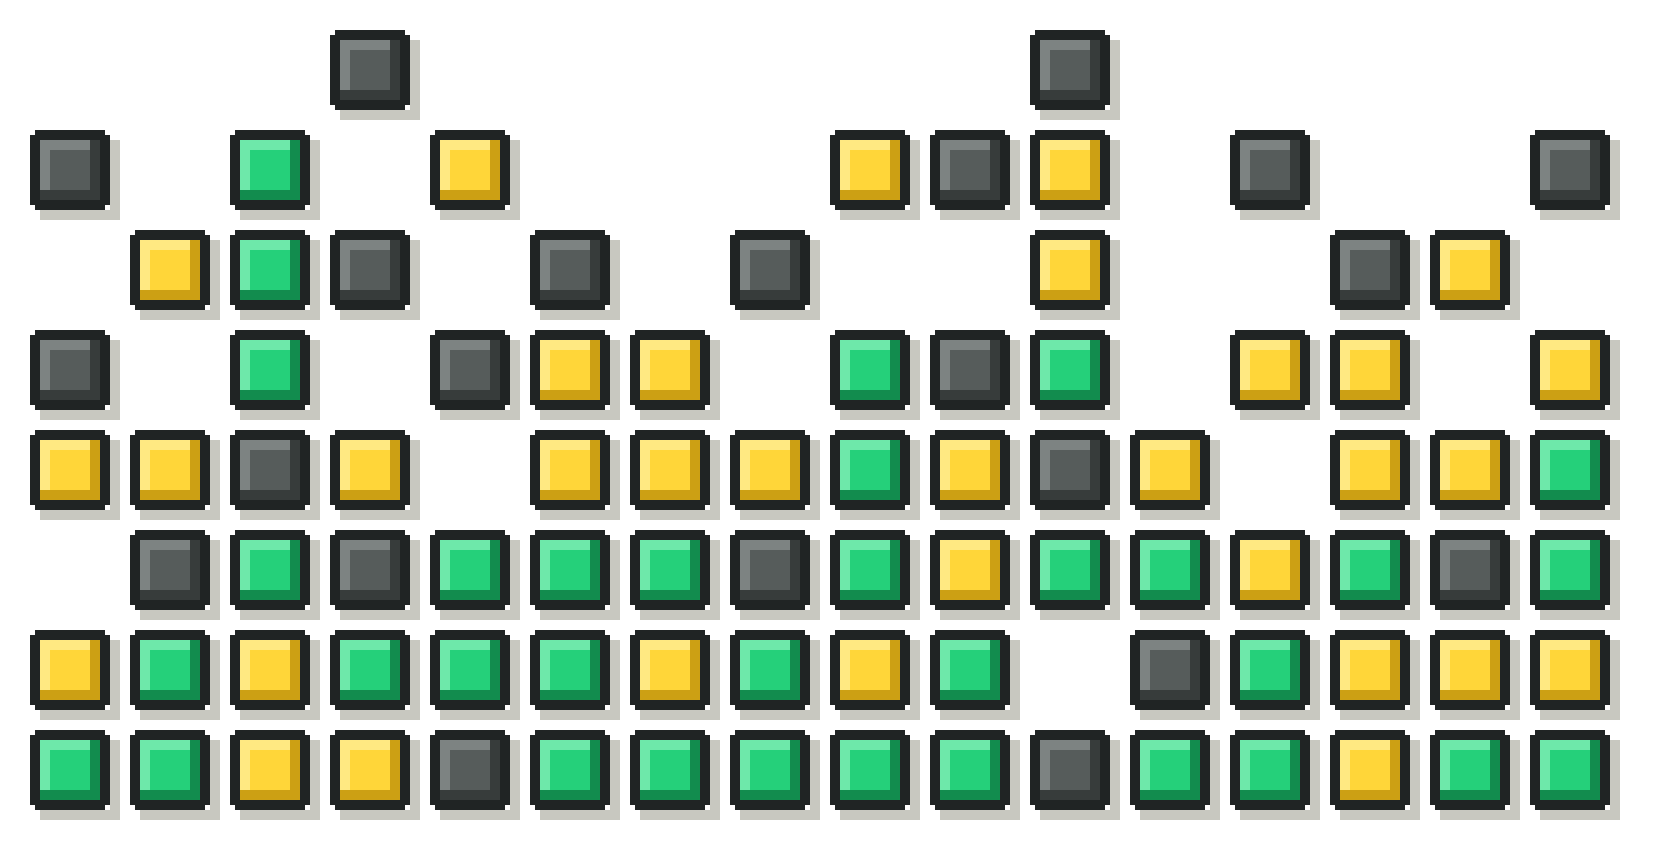
\includegraphics[
                width=\paperwidth
            ]{imagenes/wordle_pixel_art.png}%
        };
    \end{tikzpicture}

\end{titlepage}

% ------------------------- CHANGELOG ----------------------------------------

\newpage

\section*{Changelog}
\addcontentsline{toc}{section}{Changelog}

\noindent\textbf{Versión 1 (2026-10-04)}

\begin{itemize}
  \item Creación de la estructura base del documento y definición de casos de uso iniciales.
  \item Adición de referencias a interfaces gráficas e ilustraciones en los flujos de eventos.
  \item Estandarización de tablas y formatos según directrices de la asignatura.
\end{itemize}

\par\vspace{0.5cm}
\noindent\textbf{Versión 2 (2026-11-01)}

\begin{itemize}
  \item Corrección de los errores del documento anterior.
  \item Elaboración del modelo de dominio.
  \item Descripción del modelo de dominio.
\end{itemize}

\par\vspace{0.5cm}
\noindent\textbf{Versión 3 (2026-11-22)}

\begin{itemize}
  \item Corrección de los errores del modelo de dominio.
  \item Integración del plan de pruebas individual.
  \item Elaboración del diagrama de clases.
  \item Descripción del diagrama de clases.
  \item Elaboración del diagrama de comunicación.
  \item Descripción del diagrama de comunicación.
\end{itemize}

% ------------------------- INDICES ------------------------------------------

\newpage

\tableofcontents

\newpage

\listoffigures

\newpage

% ===========================================================================
% CONTENIDO
% ===========================================================================

% ------------------------- INTRODUCCION -------------------------------------

\section{Introducción}
\label{sec:introduccion}

Este documento recoge la documentación formal de los casos de uso extendidos del proyecto \textbf{Wordle}, desarrollada en el marco de la asignatura Análisis y Diseño de Sistemas de Información (ADSI).\\

Cada caso de uso analizado a lo largo del documento incluye su correspondiente descripción detallada, la identificación de los actores participantes, las precondiciones y poscondiciones asociadas, los requisitos no funcionales específicos, la especificación de los flujos de eventos y un prototipo inicial de la interfaz gráfica correspondiente.\\

A continuación, en la Ilustración~\ref{fig:diagrama_general}, se presenta el \textbf{diagrama general de casos de uso} del sistema, junto con la \textbf{jerarquía de actores}.\\

\begin{figure}[H]
    \centering
    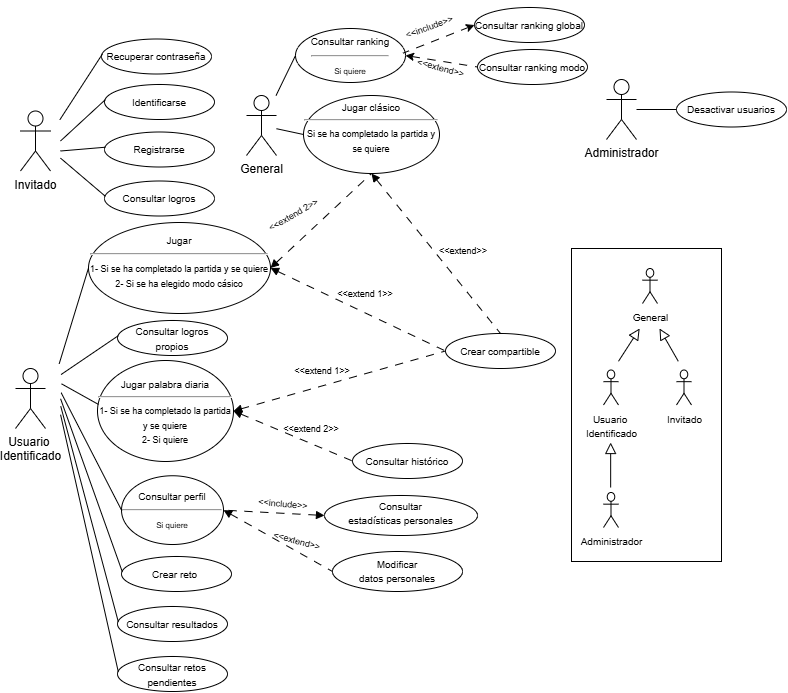
\includegraphics[width=1\linewidth]{DiagramaGeneral-Final-Los7.drawio (5).png}
    \caption{Diagrama general de casos de uso del sistema WORDLE.}
    \label{fig:diagrama_general}
\end{figure}

A modo de síntesis, las siete funcionalidades descritas en este documento y sus correspondientes responsables son los siguientes:\\

\begin{itemize}
    \item \textbf{Funcionalidad-1: Identificación y perfil.}
    Gestión del ciclo de vida de los usuarios en la plataforma. Incluye las funcionalidades de registro con elección de nombre de usuario, inicio de sesión, recuperación y cambio de contraseña. Asimismo, permite la consulta del perfil personal con métricas globales (partidas jugadas, ganadas, porcentaje de victorias, racha actual y racha máxima) y otorga al rol Administrador la capacidad de desactivar cuentas.\\
    \underline{\textbf{RESPONSABLE}}: \textit{Asier Serrano Arnaiz}\\

    \item \textbf{Funcionalidad-2: Modos de juego.}
    Selección previa a la partida entre, al menos, tres modalidades de juego distintas. Se mantiene el modo clásico (palabras de 5 letras y 6 intentos) y se introducen modos alternativos con parámetros modificados como la longitud del término, el límite de intentos o restricciones temporales de resolución.\\
    \underline{\textbf{RESPONSABLE}}: \textit{David Martínez García
}\\

    \item \textbf{Funcionalidad-3: Palabra diaria.}
    Mecanismo de juego global sincronizado donde se propone un reto único por día para toda la comunidad. Los usuarios disponen de un solo intento diario y el sistema almacena el resultado (fecha, éxito y número de intentos), garantizando el acceso al historial personal de este desafío.\\
    \underline{\textbf{RESPONSABLE}}: \textit{Lucía Sagasti Martínez
}\\

    \item \textbf{Funcionalidad-4: Retos entre usuarios.}
    Sistema asíncrono de competición entre pares. Un usuario puede desafiar a otro especificando la palabra objetivo, el límite de intentos y la fecha de caducidad. El destinatario puede consultar, aceptar y jugar los retos pendientes, quedando los resultados registrados para ambas partes. Los retos caducados no jugados a tiempo quedan inhabilitados automáticamente.\\
    \underline{\textbf{RESPONSABLE}}: \textit{Daniela Corrales Ibáñez
}\\

    \item \textbf{Funcionalidad-5: Visualización de rankings y estadísticas.}
    Plataforma de análisis de rendimiento. Proporciona clasificaciones globales y por modo de juego basadas en indicadores clave como el porcentaje de victorias, la racha máxima alcanzada o el promedio de intentos empleados. Permite además la exploración detallada de las estadísticas personales del usuario.\\
    \underline{\textbf{RESPONSABLE}}: \textit{Gonzalo de Maguregui Sánchez
}\\

    \item \textbf{Funcionalidad-6: Logros.}
    Sistema de ludificación (\textit{gamification}) que evalúa al término de cada partida la consecución de hitos específicos (p. ej., primera victoria, rachas consecutivas, acierto al primer intento o número de partidas jugadas). El usuario puede consultar el catálogo completo de logros, distinguiendo entre los obtenidos (con su fecha de adquisición) y los pendientes.\\
    \underline{\textbf{RESPONSABLE}}: \textit{Ekaitz Odriozola Díez
}\\

    \item \textbf{Funcionalidad-7: Compartir resultados.}
    Generación automática de un extracto visual para difusión. Al finalizar una partida, el sistema compone un código de casillas en formato texto que representa el desarrollo del juego sin revelar la palabra secreta. Permite incluir opcionalmente el modo de juego, la racha y los logros asociados, facilitando su copia directa para su distribución en canales externos.\\
    \underline{\textbf{RESPONSABLE}}: \textit{Aitor de Miguel Marqués
}\\
\end{itemize}

% ===========================================================================
% FUNCIONALIDAD 1
% ===========================================================================
\clearpage
\section{Casos de Uso}
\funcionalidad{1}
\newcommand{\cduGraficoFuncUno}{%
  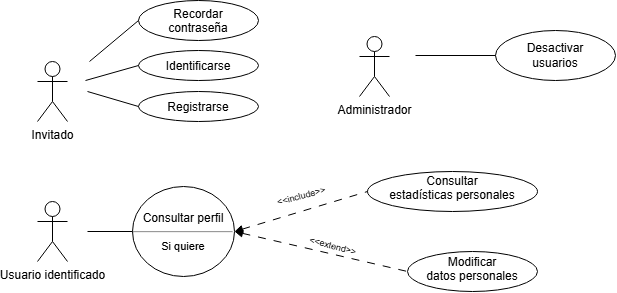
\includegraphics[
    width=0.9\linewidth,
    height=5.2cm,
    keepaspectratio
  ]{Funcionalidad1.drawio.png}%
}

% ------------------------- CASO DE USO: IDENTIFICARSE -----------------------

\casoDeUso{\cduGraficoFuncUno}
  {Identificarse}
  {Permite a un usuario acceder al sistema introduciendo su nombre de usuario y contraseña. También contempla la posibilidad de recuperar la contraseña en caso de que el usuario la haya olvidado.}
  {Invitado}
  {\begin{itemize}
    \item El usuario debe estar registrado en el sistema.
    \item La cuenta del usuario debe estar activa.
  \end{itemize}}
  {El sistema debe validar las credenciales de acceso.}
  {\begin{itemize}
    \item El usuario accede a la opción «Perfil / Login» (Ilustración 2).
    \item El sistema solicita el nombre de usuario y la contraseña (Ilustración 2).
    \item El usuario introduce sus credenciales.
    \item El sistema comprueba que el nombre de usuario existe y que la contraseña es correcta.
  \end{itemize}

  \si{Si las credenciales son incorrectas}

  \begin{itemize}
    \item El sistema muestra un mensaje de error indicando que las credenciales no son válidas.
    \item El usuario puede volver a introducir sus credenciales.
  \end{itemize}

  \si{Si el usuario ha olvidado su contraseña}

  \begin{itemize}
    \item El usuario selecciona la opción «He olvidado mi contraseña».
    \item Se ejecuta el flujo de recuperación de contraseña.
    \item Una vez finalizado el proceso, el usuario puede volver a identificarse con su nueva contraseña.
  \end{itemize}

  \si{Si las credenciales son correctas}

  \begin{itemize}
    \item El sistema comprueba que la cuenta del usuario está activa.
    \item El sistema inicia la sesión del usuario.
    \item El sistema muestra el menú principal correspondiente al usuario identificado.
  \end{itemize}}
  {\begin{itemize}
    \item Si la identificación es correcta, el usuario tendrá una sesión iniciada.
    \item Si la identificación falla, el usuario permanecerá sin identificar.
    \item Si el usuario recupera la contraseña, esta quedará actualizada en el sistema.
  \end{itemize}}
  {\begin{figure}[H]
  \centering
  \fbox{\includegraphics[width=0.85\linewidth]{imagenes/interfaz grafica/Login.png}}
  \caption{Identificarse}
  \label{fig:identificarse}
\end{figure}}

  


% ------------------------- CASO DE USO: REGISTRARSE -------------------------

\clearpage

\casoDeUso{\cduGraficoFuncUno}
  {Registrarse}
  {Permite a un nuevo usuario crear una cuenta en el sistema, indicando el nombre de usuario que desea utilizar y los datos necesarios para su registro.}
  {Invitado}
  {El usuario no debe tener ya una cuenta con el nombre de usuario elegido.}
  {El sistema debe garantizar que los nombres de usuario sean únicos.}
  {\begin{itemize}
    \item El usuario selecciona la opción «Registrarse».
    \item El sistema muestra el formulario de registro (Ilustración 3).
    \item El usuario introduce el nombre de usuario, la contraseña y los demás datos requeridos.
    \item El usuario confirma el registro.
    \item El sistema comprueba que todos los datos introducidos son válidos.
  \end{itemize}

  \si{Si los datos son incorrectos o el nombre de usuario ya existe}

  \begin{itemize}
    \item El sistema muestra un mensaje de error indicando el problema.
    \item El usuario corrige los datos y vuelve a confirmar el registro.
  \end{itemize}

  \si{Si los datos son correctos}

  \begin{itemize}
    \item El sistema crea una nueva cuenta con los datos introducidos.
    \item El sistema confirma que el registro se ha realizado correctamente.
  \end{itemize}}
  {\begin{itemize}
    \item Si el registro se completa correctamente, se crea una nueva cuenta de usuario.
    \item Si el registro falla, no se crea ninguna cuenta.
  \end{itemize}}
{\begin{figure}[H]
  \centering
  \fbox{\includegraphics[width=0.85\linewidth]{Login.png}}
  \caption{Registrarse}
  \label{fig:registrarse}
\end{figure}}

% ------------------------- CASO DE USO: CONSULTAR PERFIL --------------------

\clearpage

\casoDeUso{\cduGraficoFuncUno}
  {Consultar perfil}
  {Permite a un usuario identificado acceder a su perfil personal, desde el que podrá consultar sus estadísticas personales y modificar sus datos.}
  {Usuario identificado}
  {El usuario debe haber iniciado sesión.}
  {\begin{itemize}
    \item La información mostrada debe corresponder al usuario identificado.
    \item El acceso al perfil debe estar restringido a usuarios identificados.
  \end{itemize}}
  {\begin{itemize}
    \item El usuario accede al menú principal.
    \item El usuario selecciona la opción «Perfil» (Ilustración 4).
    \item El sistema recupera los datos asociados a la cuenta del usuario.
    \item El sistema muestra la información del perfil (Ilustración 4).
  \end{itemize}

  \si{Si el usuario selecciona «Consultar estadísticas personales»}

  \begin{itemize}
    \item Se ejecuta el caso de uso «Consultar estadísticas personales».
  \end{itemize}

  \si{Si el usuario selecciona «Modificar datos personales»}

  \begin{itemize}
    \item Se ejecuta el caso de uso «Modificar datos personales».
  \end{itemize}

  \si{Si el usuario decide salir del perfil}

  \begin{itemize}
    \item El sistema vuelve al menú principal.
  \end{itemize}}
  {\begin{itemize}
    \item El usuario habrá podido acceder a su perfil.
    \item No se modificarán datos si el usuario no ejecuta ninguna operación de modificación.
  \end{itemize}}
{\begin{figure}[H]
  \centering
  \fbox{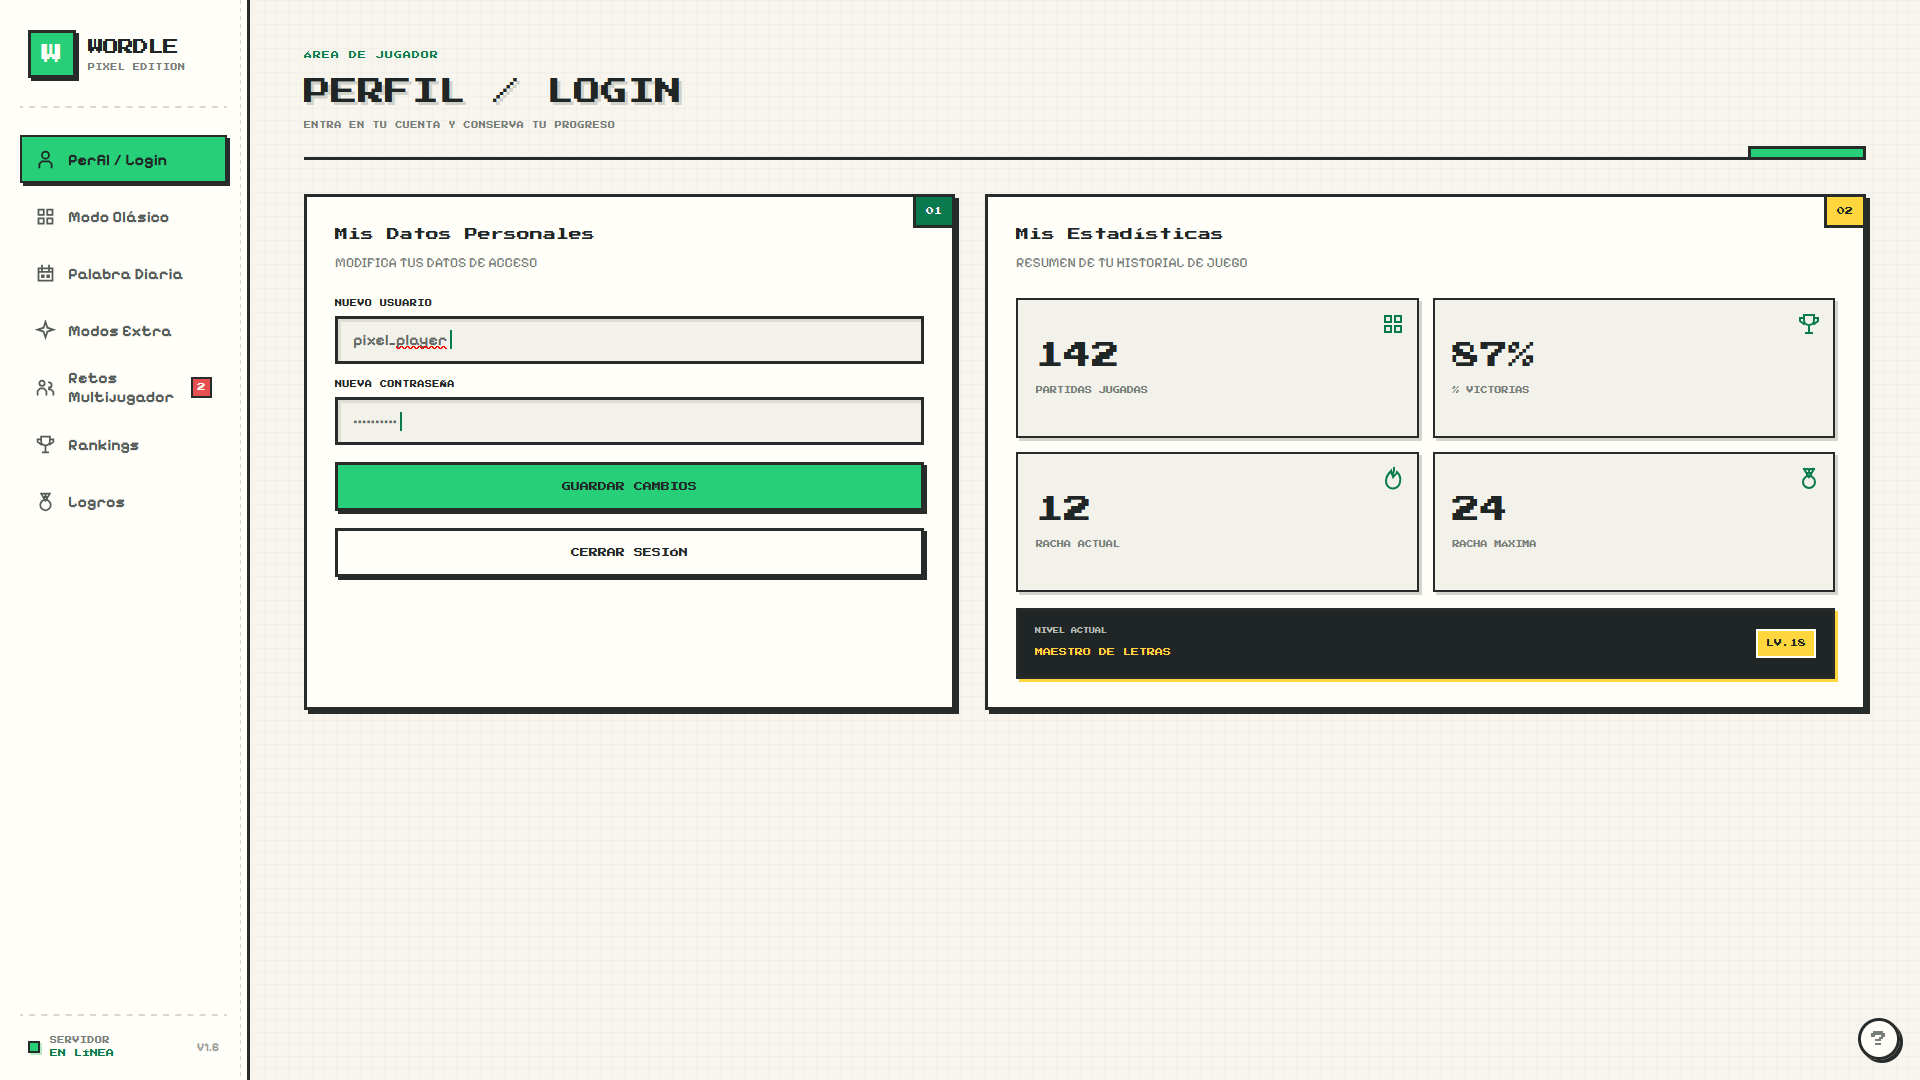
\includegraphics[width=0.85\linewidth]{Mis datos.png}}
  \caption{Ver perfil}
  \label{fig:ver-perfil}
\end{figure}}

% ------------------------- CASO DE USO: ESTADISTICAS ------------------------

\clearpage

\casoDeUso{\cduGraficoFuncUno}
  {Consultar estadísticas personales}
  {Permite a un usuario identificado consultar sus estadísticas de juego, incluyendo el número de partidas jugadas y ganadas, el porcentaje de victorias, la racha actual de victorias y la racha máxima.}
  {Usuario identificado}
  {\begin{itemize}
    \item El usuario debe haber iniciado sesión.
    \item El usuario debe acceder a su perfil.
  \end{itemize}}
  {Las estadísticas mostradas deben corresponder a los resultados registrados del usuario.}
  {\begin{itemize}
    \item El usuario accede a su perfil.
    \item El usuario selecciona la opción «Consultar estadísticas personales».
    \item El sistema recupera las partidas y los resultados asociados al usuario.
    \item El sistema calcula o recupera las estadísticas correspondientes:
    \begin{itemize}
      \item Número de partidas jugadas.
      \item Número de partidas ganadas.
      \item Porcentaje de victorias.
      \item Racha actual de victorias.
      \item Racha máxima de victorias.
    \end{itemize}
    \item El sistema muestra las estadísticas personales (Ilustración 5).
    \item El usuario selecciona la opción «Volver».
    \item El sistema regresa a la pantalla del perfil.
  \end{itemize}}
  {\begin{itemize}
    \item El usuario habrá consultado sus estadísticas personales.
    \item No se modificará la información almacenada del usuario.
  \end{itemize}}
{\begin{figure}[H]
  \centering
  \fbox{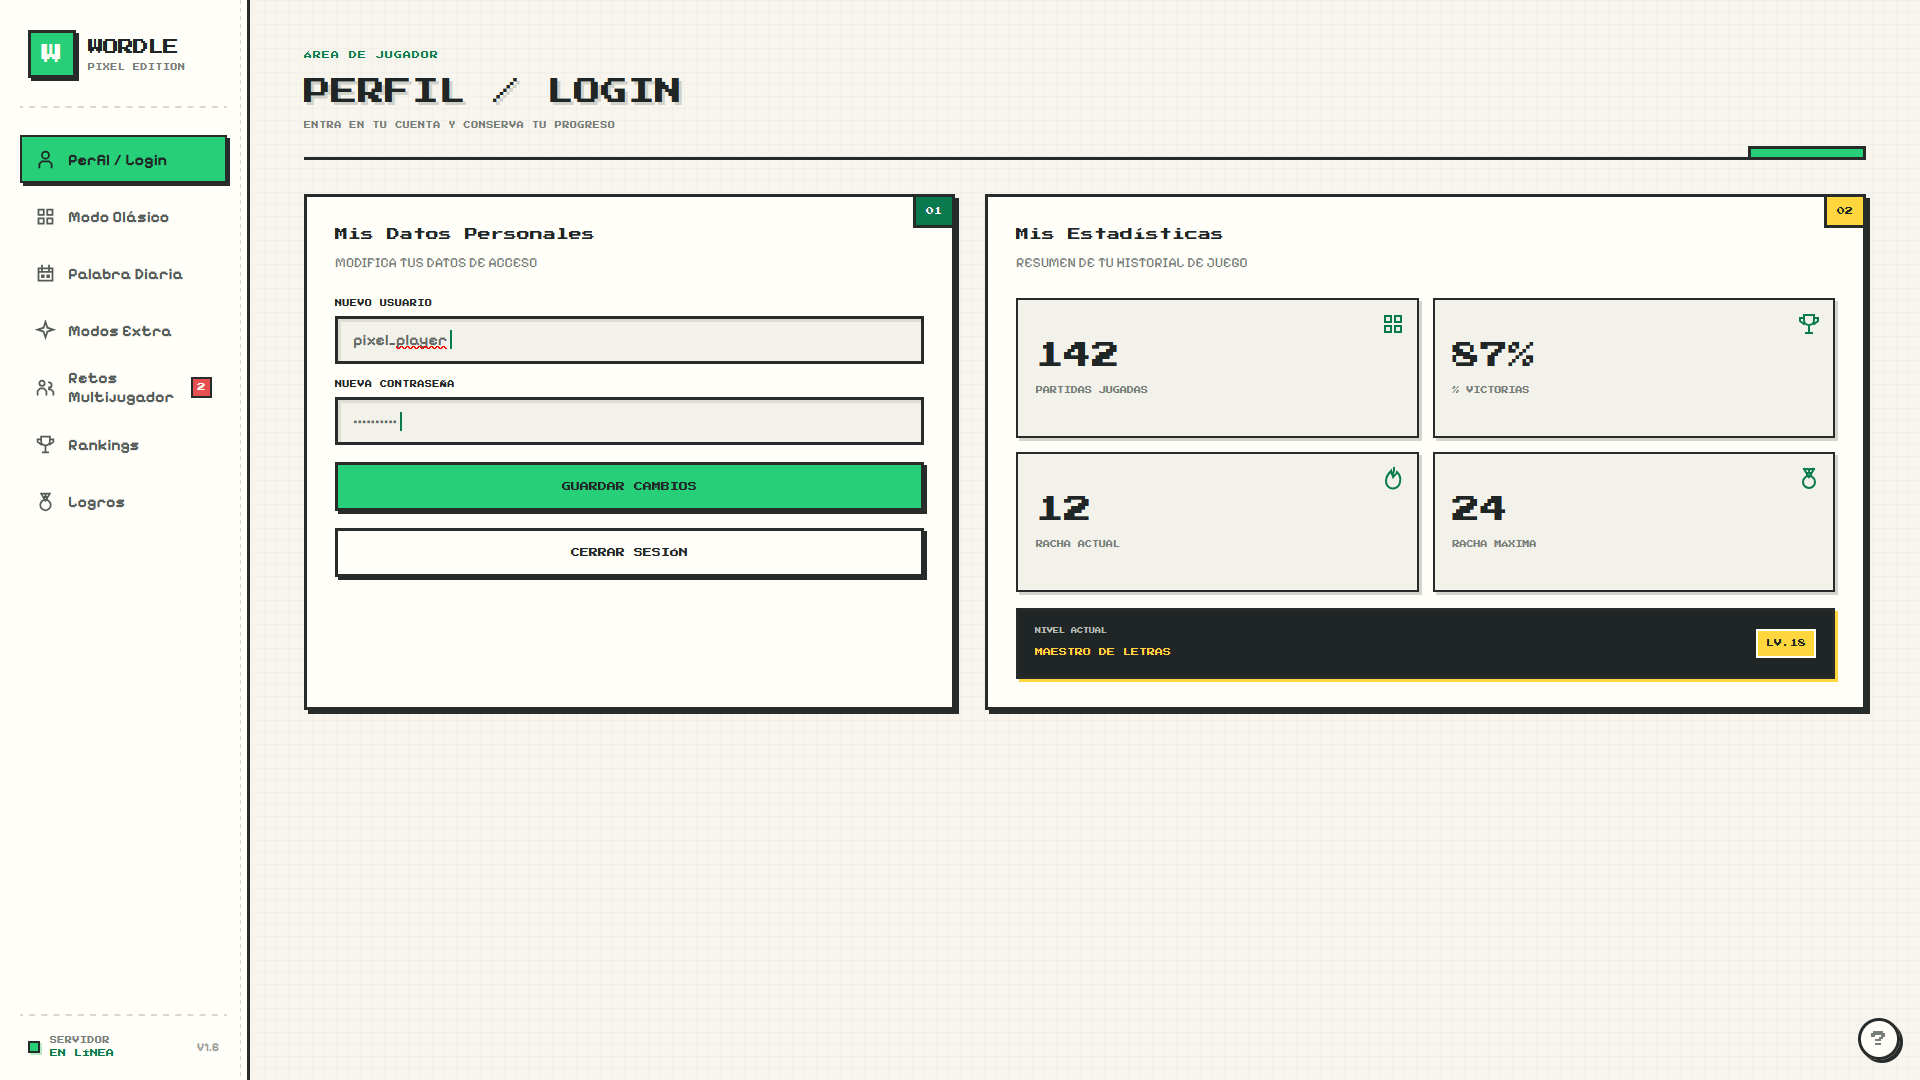
\includegraphics[width=0.85\linewidth]{Mis datos.png}}
  \caption{Estadísticas personales}
  \label{fig:estadisticas-personales}
\end{figure}}
  

% ------------------------- CASO DE USO: MODIFICAR DATOS ---------------------

\clearpage

\casoDeUso{\cduGraficoFuncUno}
  {Modificar datos personales}
  {Permite a un usuario identificado modificar los datos asociados a su cuenta.}
  {Usuario identificado}
  {\begin{itemize}
    \item El usuario debe haber iniciado sesión.
    \item El usuario debe acceder a su perfil.
  \end{itemize}}
  {\begin{itemize}
    \item El sistema debe validar los datos introducidos.
    \item El sistema debe garantizar que los nombres de usuario sean únicos si se permite modificarlos.
  \end{itemize}}
  {\begin{itemize}
    \item El usuario accede a su perfil.
    \item El usuario selecciona la opción «Modificar datos personales».
    \item El sistema muestra los datos actuales del usuario y permite editarlos (Ilustración 6).
    \item El usuario selecciona los datos que desea modificar.
    \item El sistema permite editar los campos seleccionados.
  \end{itemize}

  \si{Si el usuario desea modificar sus datos personales}

  \begin{itemize}
    \item El usuario modifica los datos personales que desea cambiar.
    \item El usuario confirma los cambios.
    \item El sistema comprueba que los datos introducidos son válidos.
  \end{itemize}

  \si{Si el usuario desea cambiar su contraseña}

  \begin{itemize}
    \item El usuario selecciona la opción «Cambiar contraseña».
    \item El sistema solicita la contraseña actual, la nueva contraseña y su confirmación.
    \item El usuario introduce los datos solicitados.
    \item El sistema comprueba que la contraseña actual es correcta y que la nueva contraseña cumple los requisitos establecidos.
    \item El usuario confirma el cambio.
  \end{itemize}

  \si{Si los datos introducidos no son válidos}

  \begin{itemize}
    \item El sistema muestra un mensaje de error indicando el problema.
  \end{itemize}

  \si{Si los datos son válidos}

  \begin{itemize}
    \item El sistema actualiza los datos personales o la contraseña, según corresponda.
    \item El sistema confirma que los cambios se han guardado correctamente.
    \item El sistema vuelve a la pantalla del perfil.
  \end{itemize}}
  {\begin{itemize}
    \item Si la operación finaliza correctamente, los datos personales seleccionados estarán actualizados.
    \item Si el usuario cambia la contraseña correctamente, la nueva contraseña sustituirá a la anterior.
    \item Si se produce un error, los datos anteriores se conservarán.
  \end{itemize}}
{\begin{figure}[H]
  \centering
  \fbox{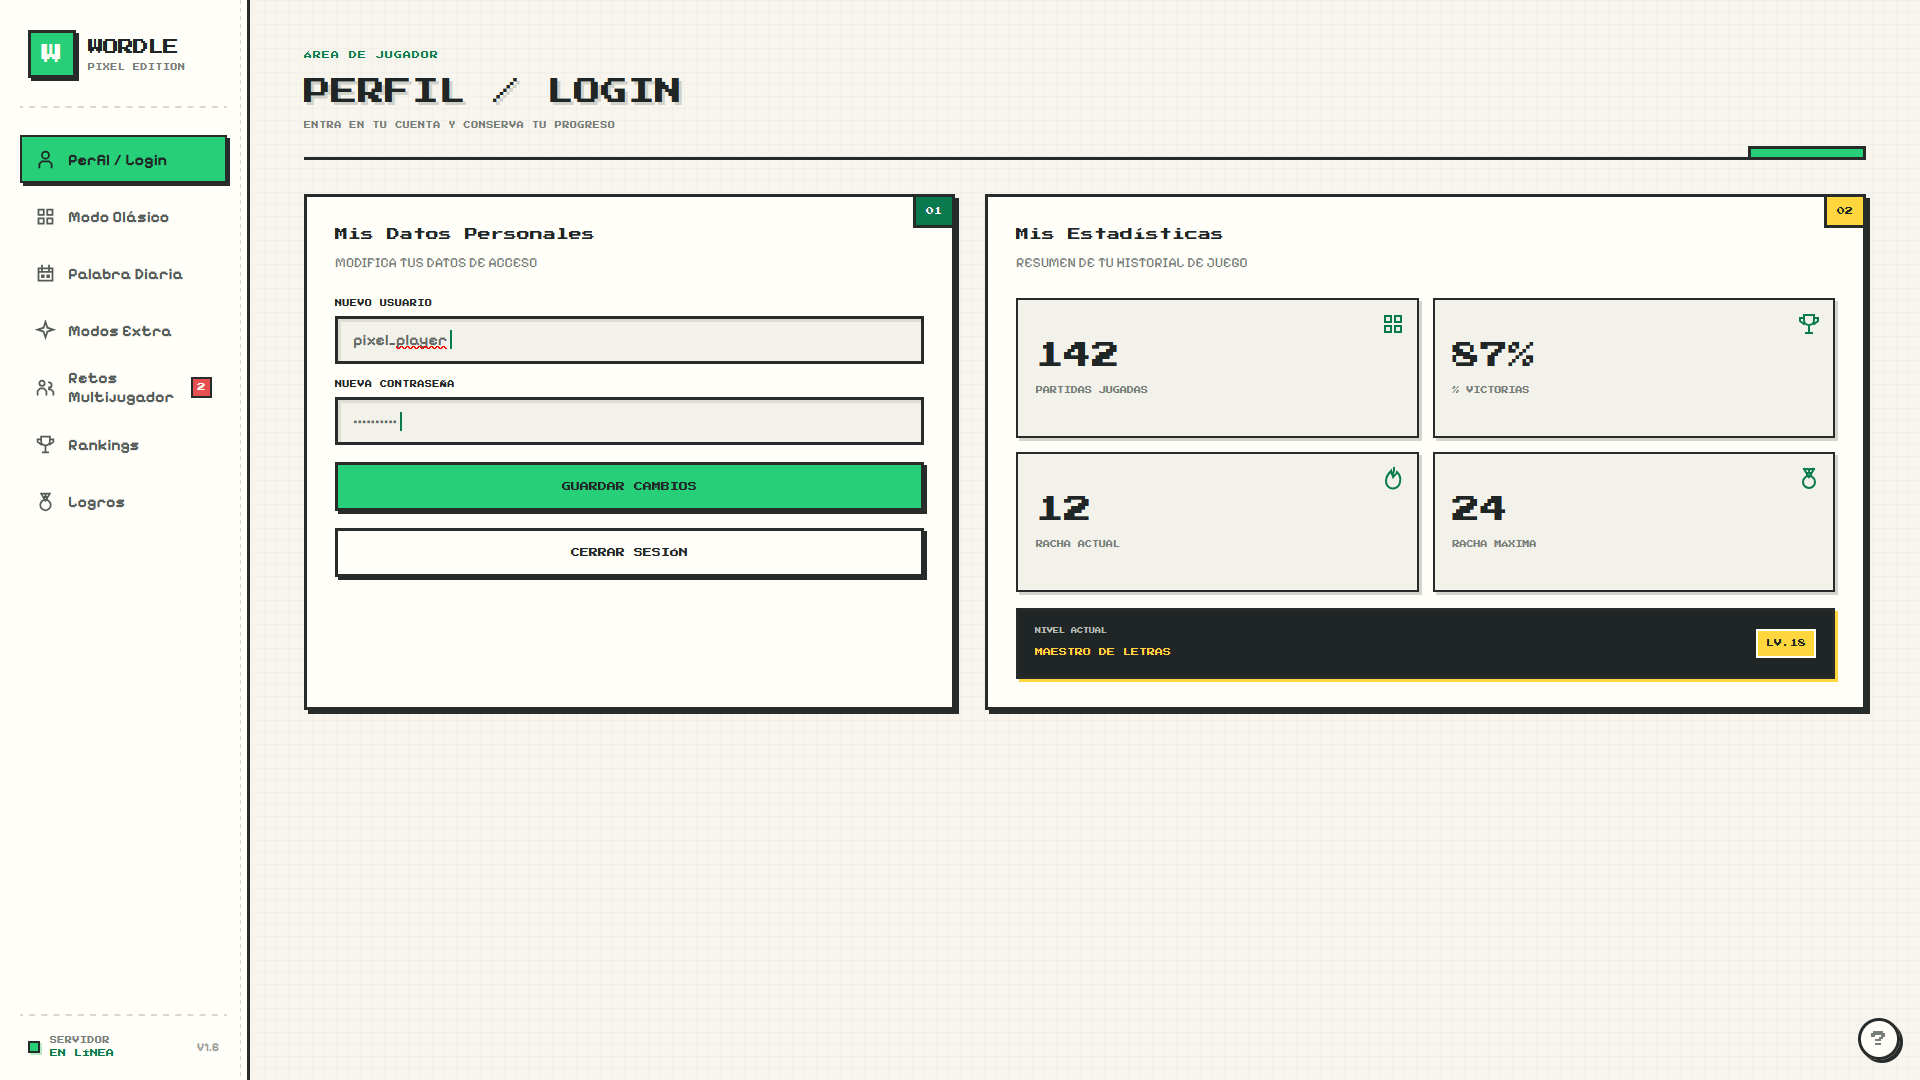
\includegraphics[width=0.85\linewidth]{Mis datos.png}}
  \caption{Estadísticas personales}
  \label{fig:estadisticas-personales}
\end{figure}}

% ------------------------- CASO DE USO: DESACTIVAR USUARIOS ---------------

\clearpage

\casoDeUso{\cduGraficoFuncUno}
  {Desactivar usuarios}
  {Permite al administrador desactivar la cuenta de un usuario para impedir que pueda utilizar el sistema.}
  {Administrador}
  {\begin{itemize}
    \item El administrador debe haber iniciado sesión y ser administrador.
    \item El usuario que se desea desactivar debe existir en el sistema.
  \end{itemize}}
  {\begin{itemize}
    \item El acceso a esta funcionalidad debe estar restringido al administrador.
    \item El sistema debe garantizar la integridad de los datos de los usuarios.
  \end{itemize}}
  {\begin{itemize}
    \item El administrador accede a la opción de gestión de usuarios.
    \item El sistema muestra la lista de usuarios registrados.
    \item El administrador selecciona el usuario que desea desactivar.
    \item El sistema muestra los datos del usuario seleccionado.
    \item El administrador selecciona la opción «Desactivar usuario».
    \item El sistema solicita la confirmación de la operación.
  \end{itemize}

  \si{Si el administrador cancela la operación}

  \begin{itemize}
    \item El sistema cancela la desactivación.
    \item El sistema vuelve a la lista de usuarios.
  \end{itemize}

  \si{Si el administrador confirma la operación}

  \begin{itemize}
    \item El sistema comprueba que el usuario puede ser desactivado.
    \item El sistema cambia el estado de la cuenta a desactivada.
    \item El sistema confirma que la operación se ha realizado correctamente.
    \item El sistema vuelve a la lista de usuarios.
  \end{itemize}}
  {\begin{itemize}
    \item Si la operación se completa correctamente, la cuenta del usuario quedará desactivada.
    \item El usuario desactivado no podrá identificarse en el sistema.
    \item Los datos y las estadísticas del usuario se conservarán.
  \end{itemize}}
  {}

% ===========================================================================
% FUNCIONALIDAD 2
% ===========================================================================
\clearpage
\funcionalidad{2}
\newcommand{\cduGraficoFuncDos}{%
  
\includegraphics[
    width=0.9\linewidth,
    height=5.2cm,
    keepaspectratio
  ]{Funcionalidad2.png}%
}

% ------------------------- JUGAR CLASICO ------------------------------------



\casoDeUso{\cduGraficoFuncDos}
  {Jugar clásico}
  {El usuario puede seleccionar la pestaña del modo clásico de juego. Además, tiene el poder de escribir palabras y de enviarlas para poder ganar la partida. En caso de que el usuario que juegue esté registrado, se almacenará el resultado obtenido, incluyendo la fecha, si se ha resuelto correctamente y el número de intentos utilizados.}
  {General}
  {No hay.}
  {Ninguno}
  {\begin{enumerate}
    \item El usuario, sea invitado o registrado, entra a la página del juego y selecciona el modo clásico (Ilustración 7).
    \item El usuario juega la partida (Ilustración 8).
    \item El usuario termina la partida:
    \begin{itemize}
      \item a. El usuario gana.
      \item b. El usuario pierde.
    \end{itemize}
  \end{enumerate}}
  {Si el usuario está registrado se guarda la partida en el historial de juegos, en cambio si juega como invitado, la partida no se guarda.}
{\begin{figure}[H]
  \centering
  \fbox{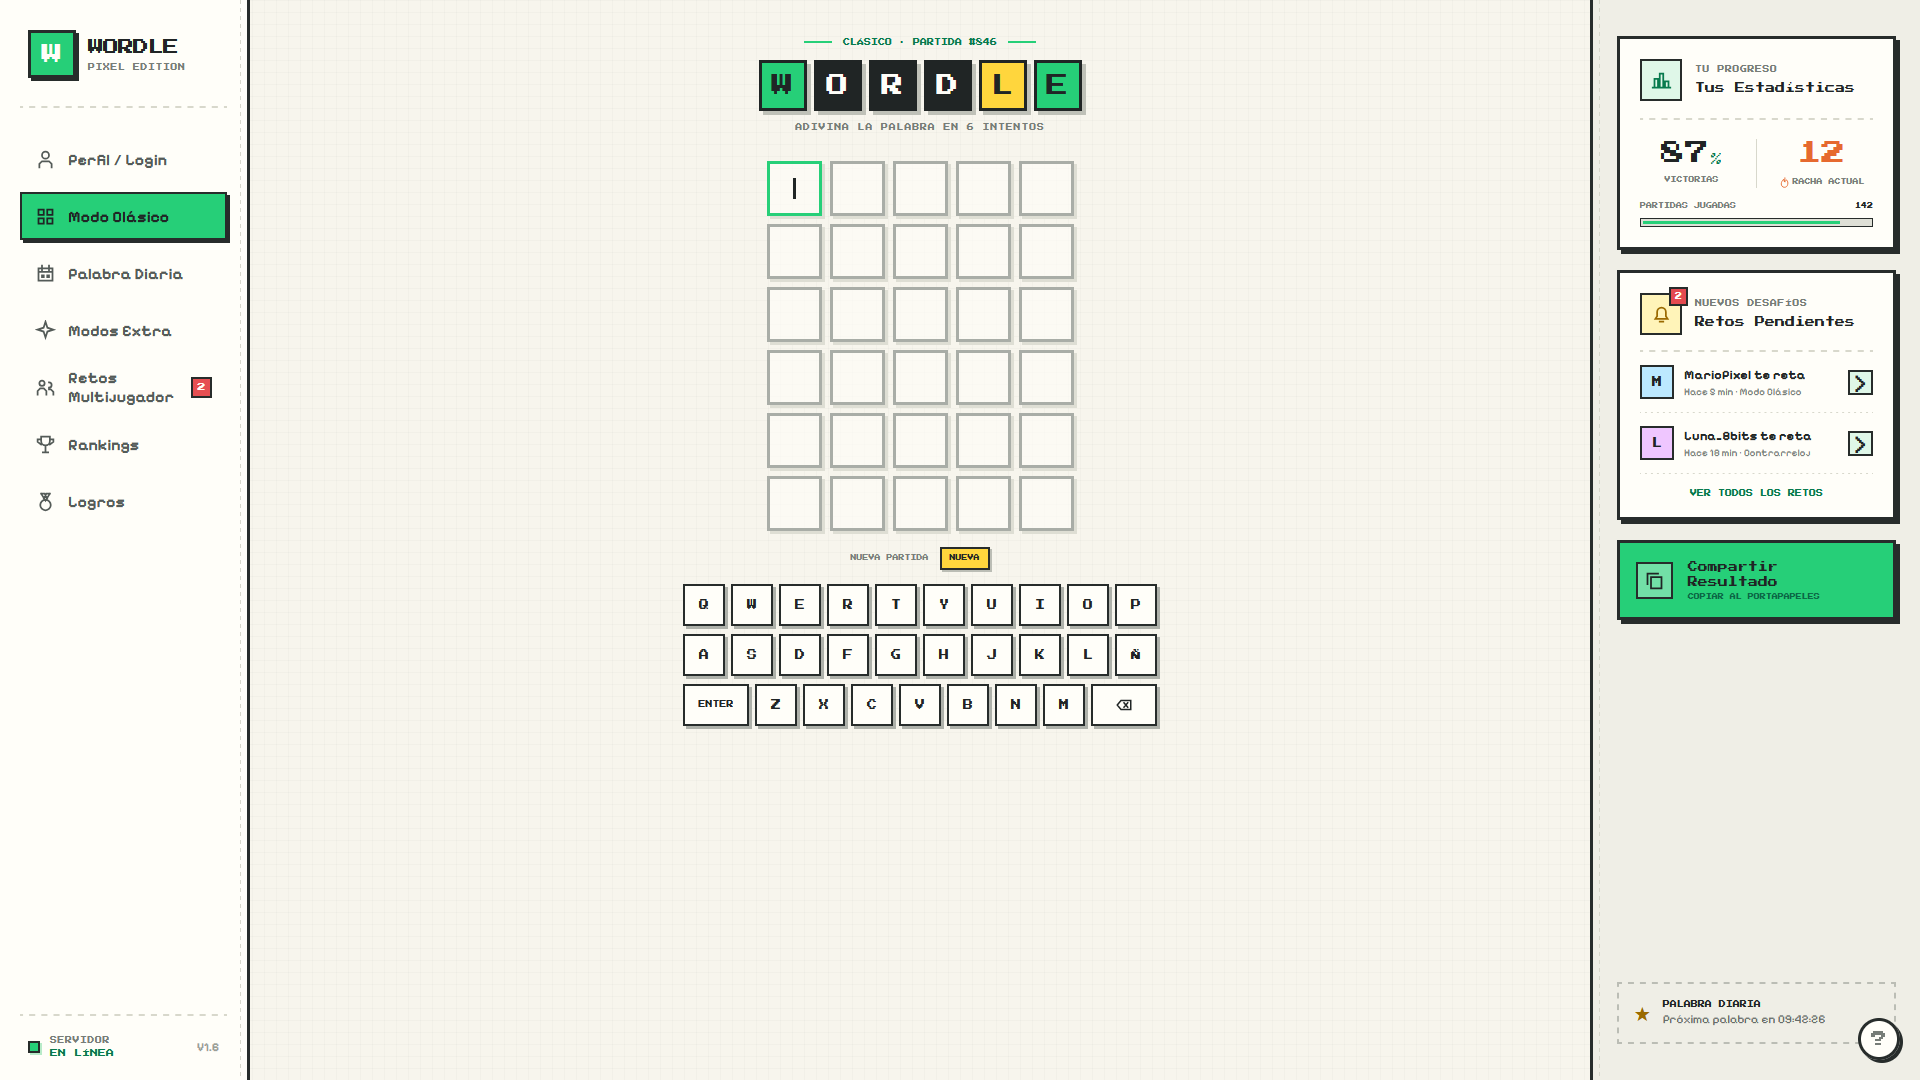
\includegraphics[width=0.85\linewidth]{Clasico.png}}
  \caption{Modo clásico}
  \label{fig:modo-clasico}
\end{figure}
\begin{figure}[H]
  \centering
  \fbox{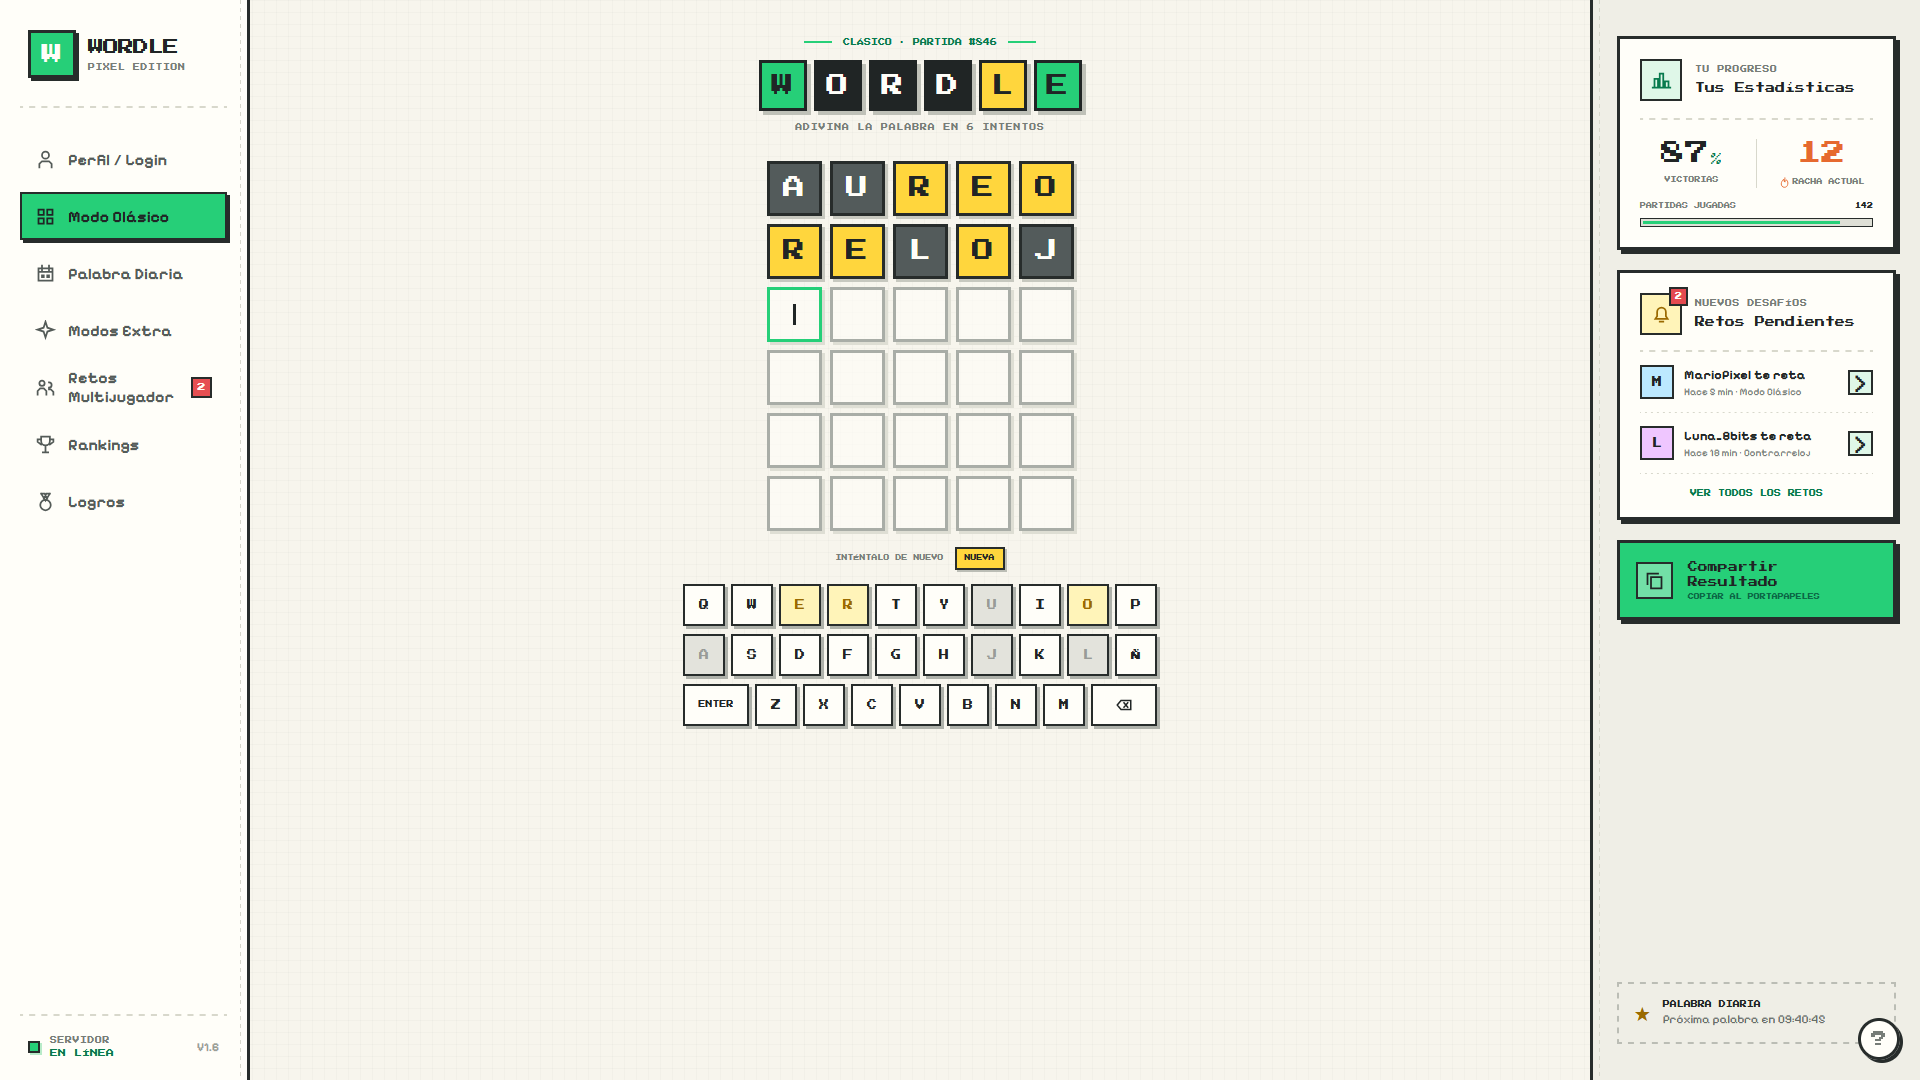
\includegraphics[width=0.85\linewidth]{Clasico en curso.png}}
  \caption{Modo clásico en partida}
  \label{fig:modo-clasico-partida}
\end{figure}}

% ------------------------- JUGAR 2 ------------------------------------------

\clearpage

\casoDeUso{\cduGraficoFuncDos}
  {Jugar 2}
  {El usuario registrado es capaz de seleccionar la pestaña del modo "jugar 2". Además, tiene el poder de escribir palabras y de enviarlas para poder terminar la partida. En caso de jugar se almacenará el resultado obtenido, incluyendo la fecha, si se ha resuelto correctamente y el número de intentos utilizados.}
  {Usuario.}
  {Estar identificado como usuario.}
  {Ninguno}
  {\begin{enumerate}
    \item El usuario entra a la página del juego y selecciona el modo de juego “jugar 2”.
    \item El usuario juega la partida (Ilustración 9).
    \item El usuario termina la partida:
    \begin{itemize}
      \item a. El usuario gana.
      \item b. El usuario pierde.
    \end{itemize}
  \end{enumerate}}
  {Se guarda la partida en el historial de juegos.}
  {\begin{figure}[H]
  \centering
  \fbox{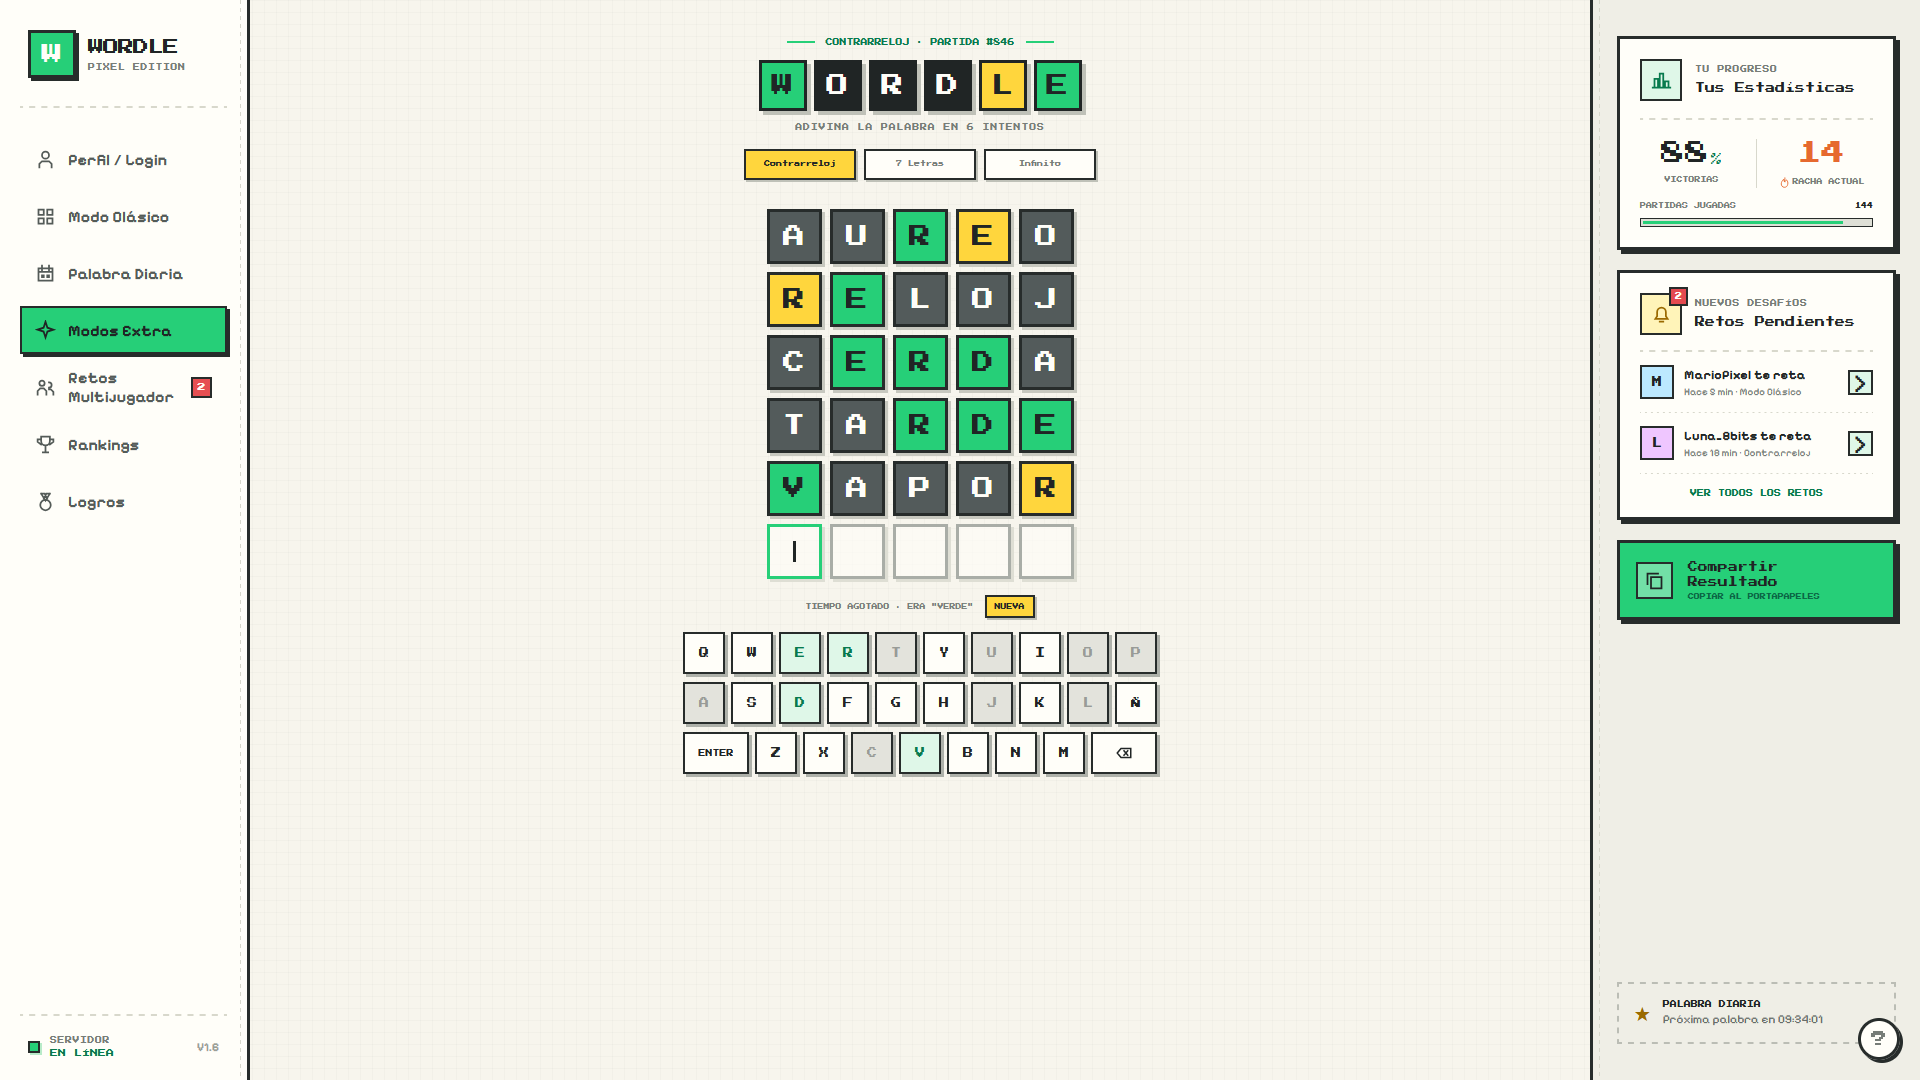
\includegraphics[width=0.85\linewidth]{Contrareloj.png}}
  \caption{Contrarreloj}
  \label{fig:contrareloj}
\end{figure}
\begin{figure}[H]
  \centering
  \fbox{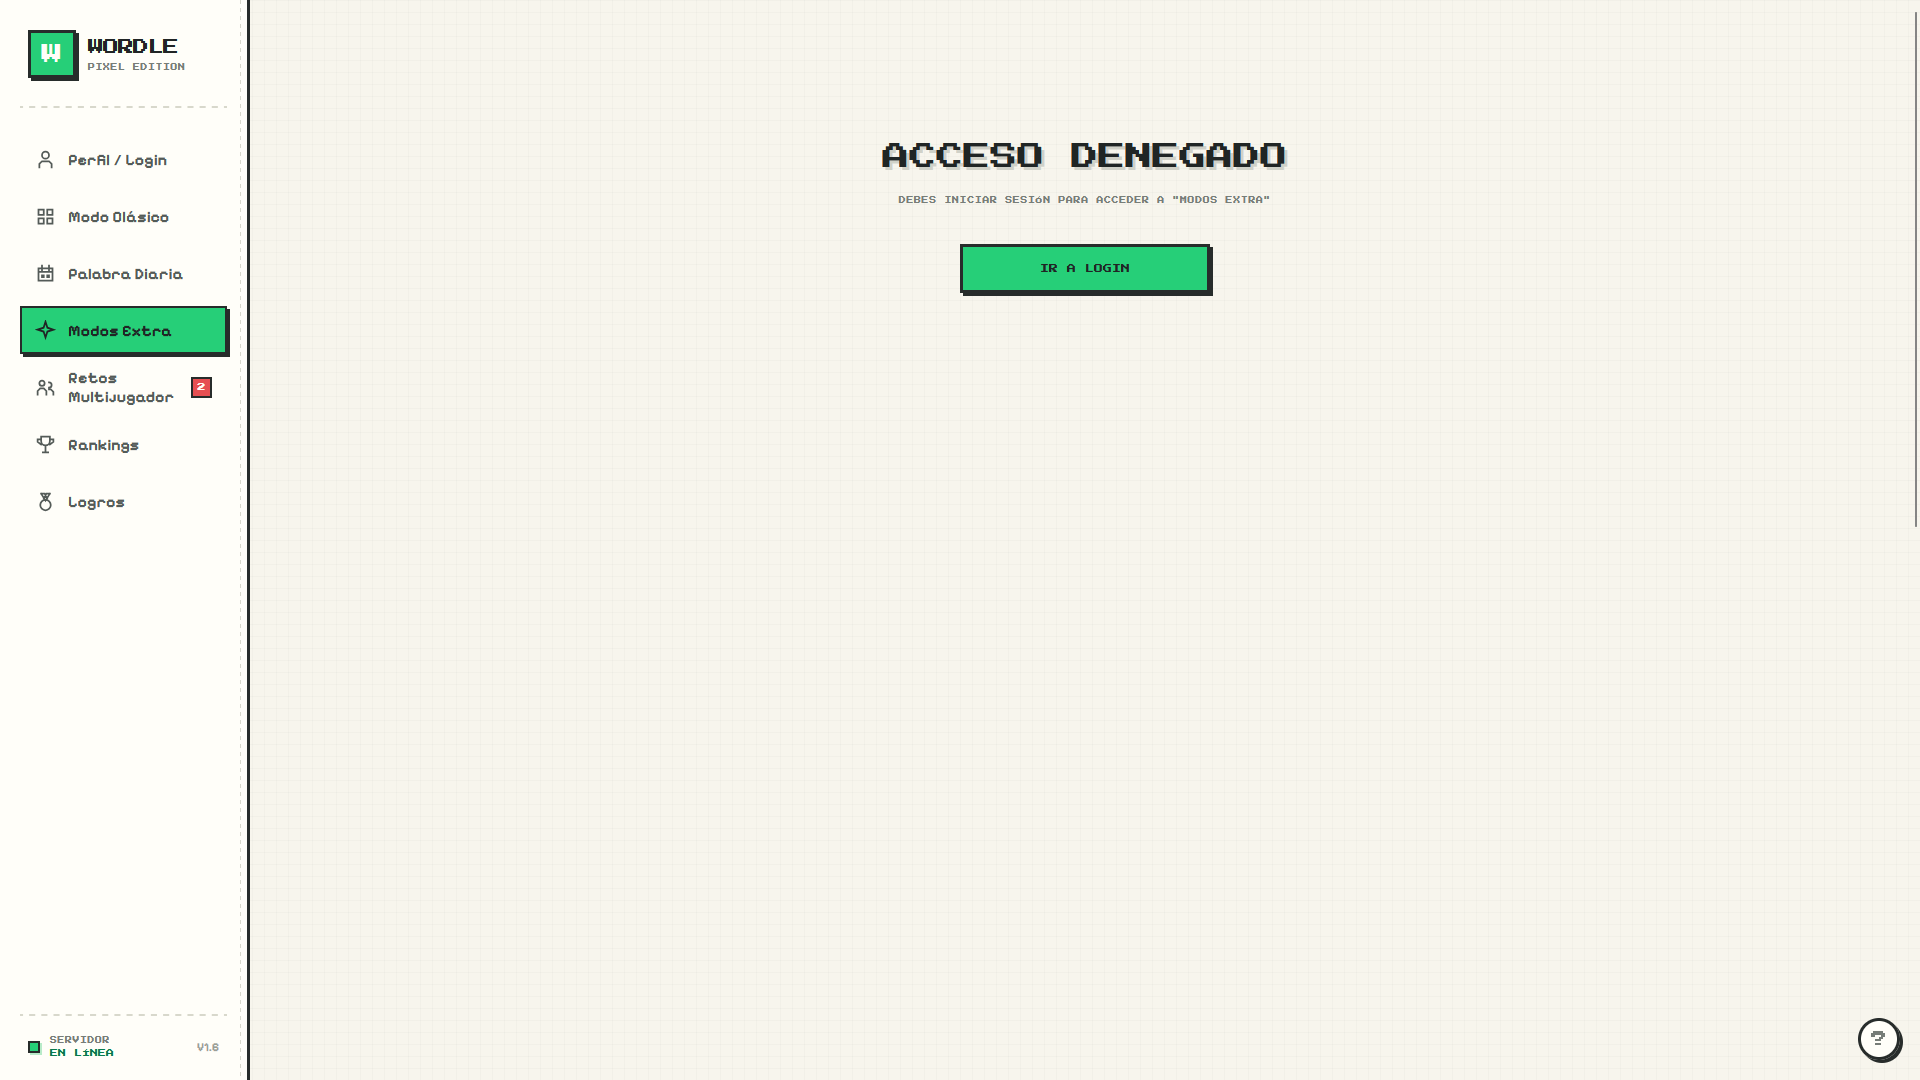
\includegraphics[width=0.85\linewidth]{Modos extra denied.png}}
  \caption{La opción "Modos extra" no disponible para invitado}
  \label{fig:modos-extra-denied-1}
\end{figure}}

% ------------------------- JUGAR 3 ------------------------------------------

\clearpage

\casoDeUso{\cduGraficoFuncDos}
  {Jugar 3}
  {El usuario registrado es capaz de seleccionar la pestaña del modo "jugar 3". Además, tiene el poder de escribir palabras y de enviarlas para poder terminar la partida. En caso de jugar se almacenará el resultado obtenido, incluyendo la fecha, si se ha resuelto correctamente y el número de intentos utilizados.}
  {Usuario.}
  {Estar identificado como usuario.}
  {Ninguno}
  {\begin{enumerate}
    \item El usuario entra a la página del juego y selecciona el modo de juego “jugar 3”.
    \item El usuario juega la partida (Ilustración 11).
    \item El usuario termina la partida:
    \begin{itemize}
      \item a. El usuario gana.
      \item b. El usuario pierde.
    \end{itemize}
  \end{enumerate}}
  {Se guarda la partida en el historial de juegos.}
  {\begin{figure}[H]
  \centering
  \fbox{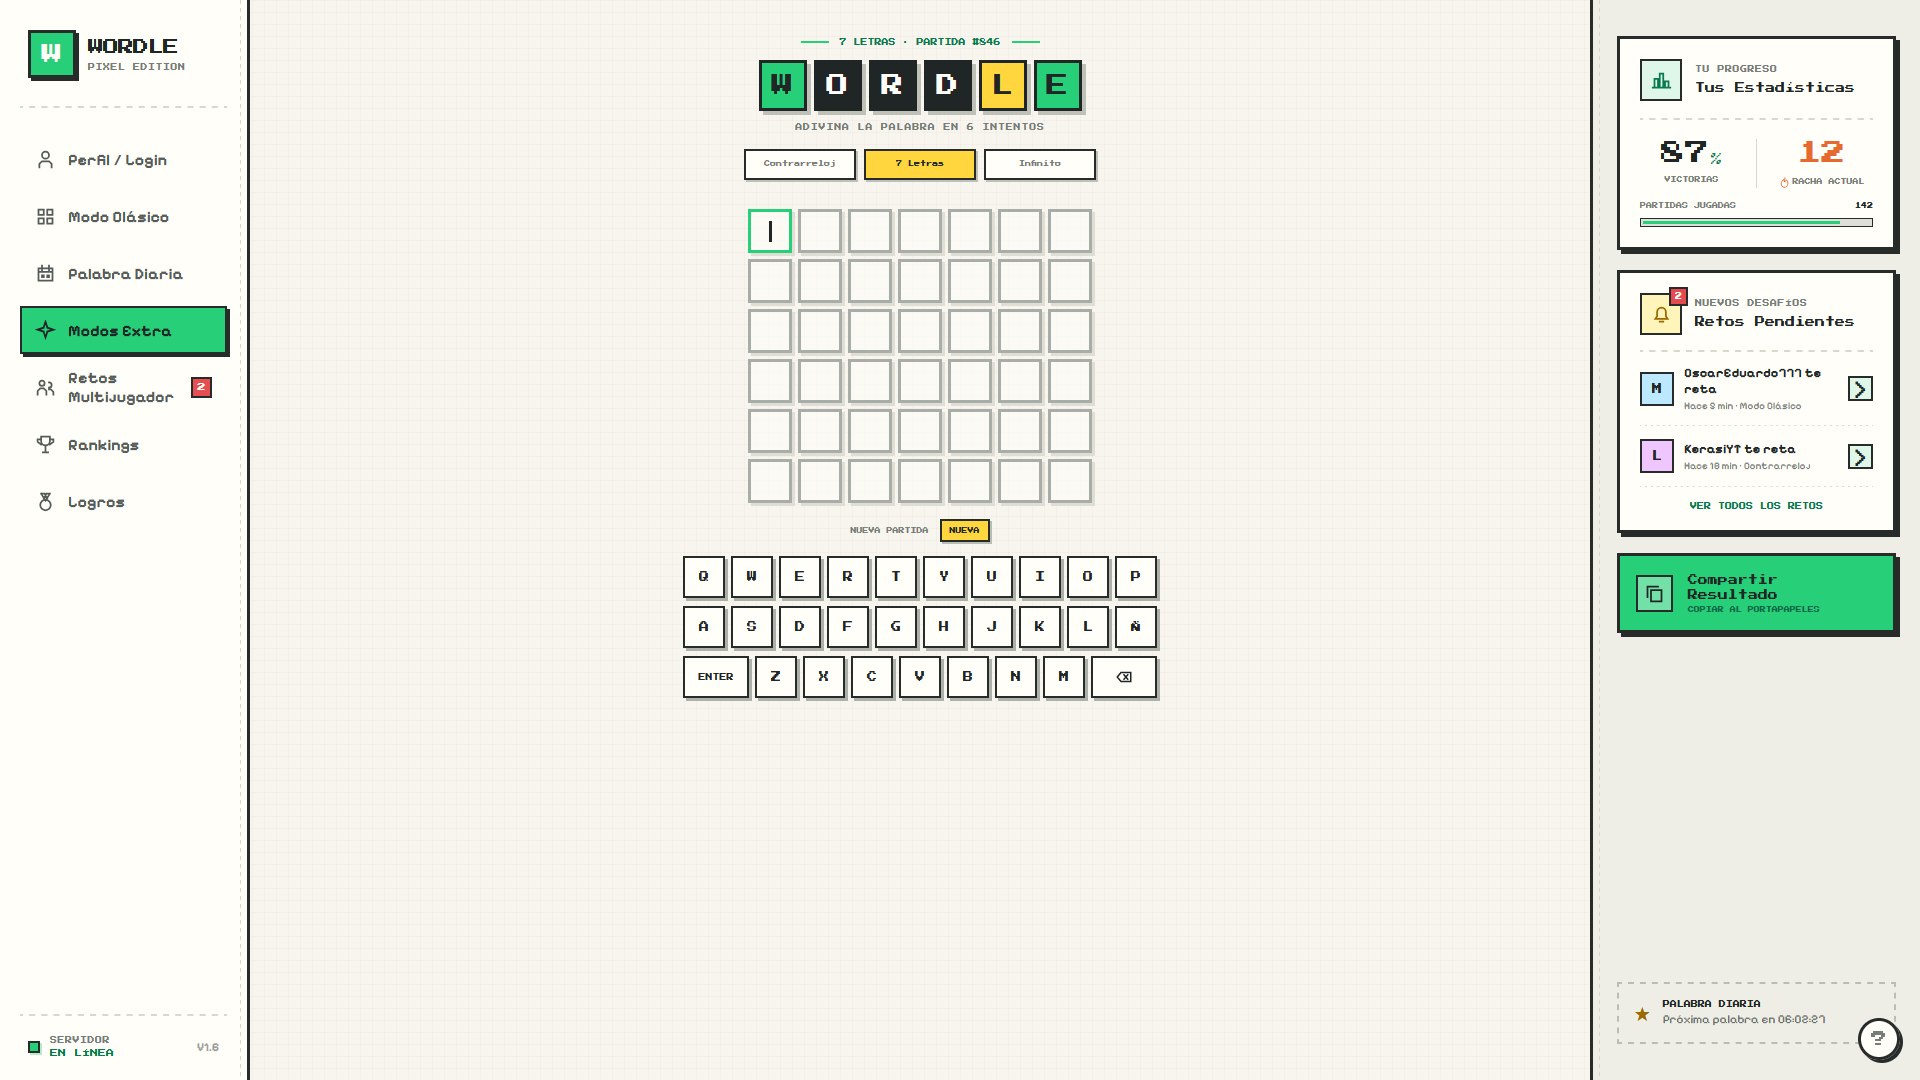
\includegraphics[width=0.85\linewidth]{7 Letras.png}}
  \caption{7 Letras}
  \label{fig:siete-letras}
\end{figure}
\begin{figure}[H]
  \centering
  \fbox{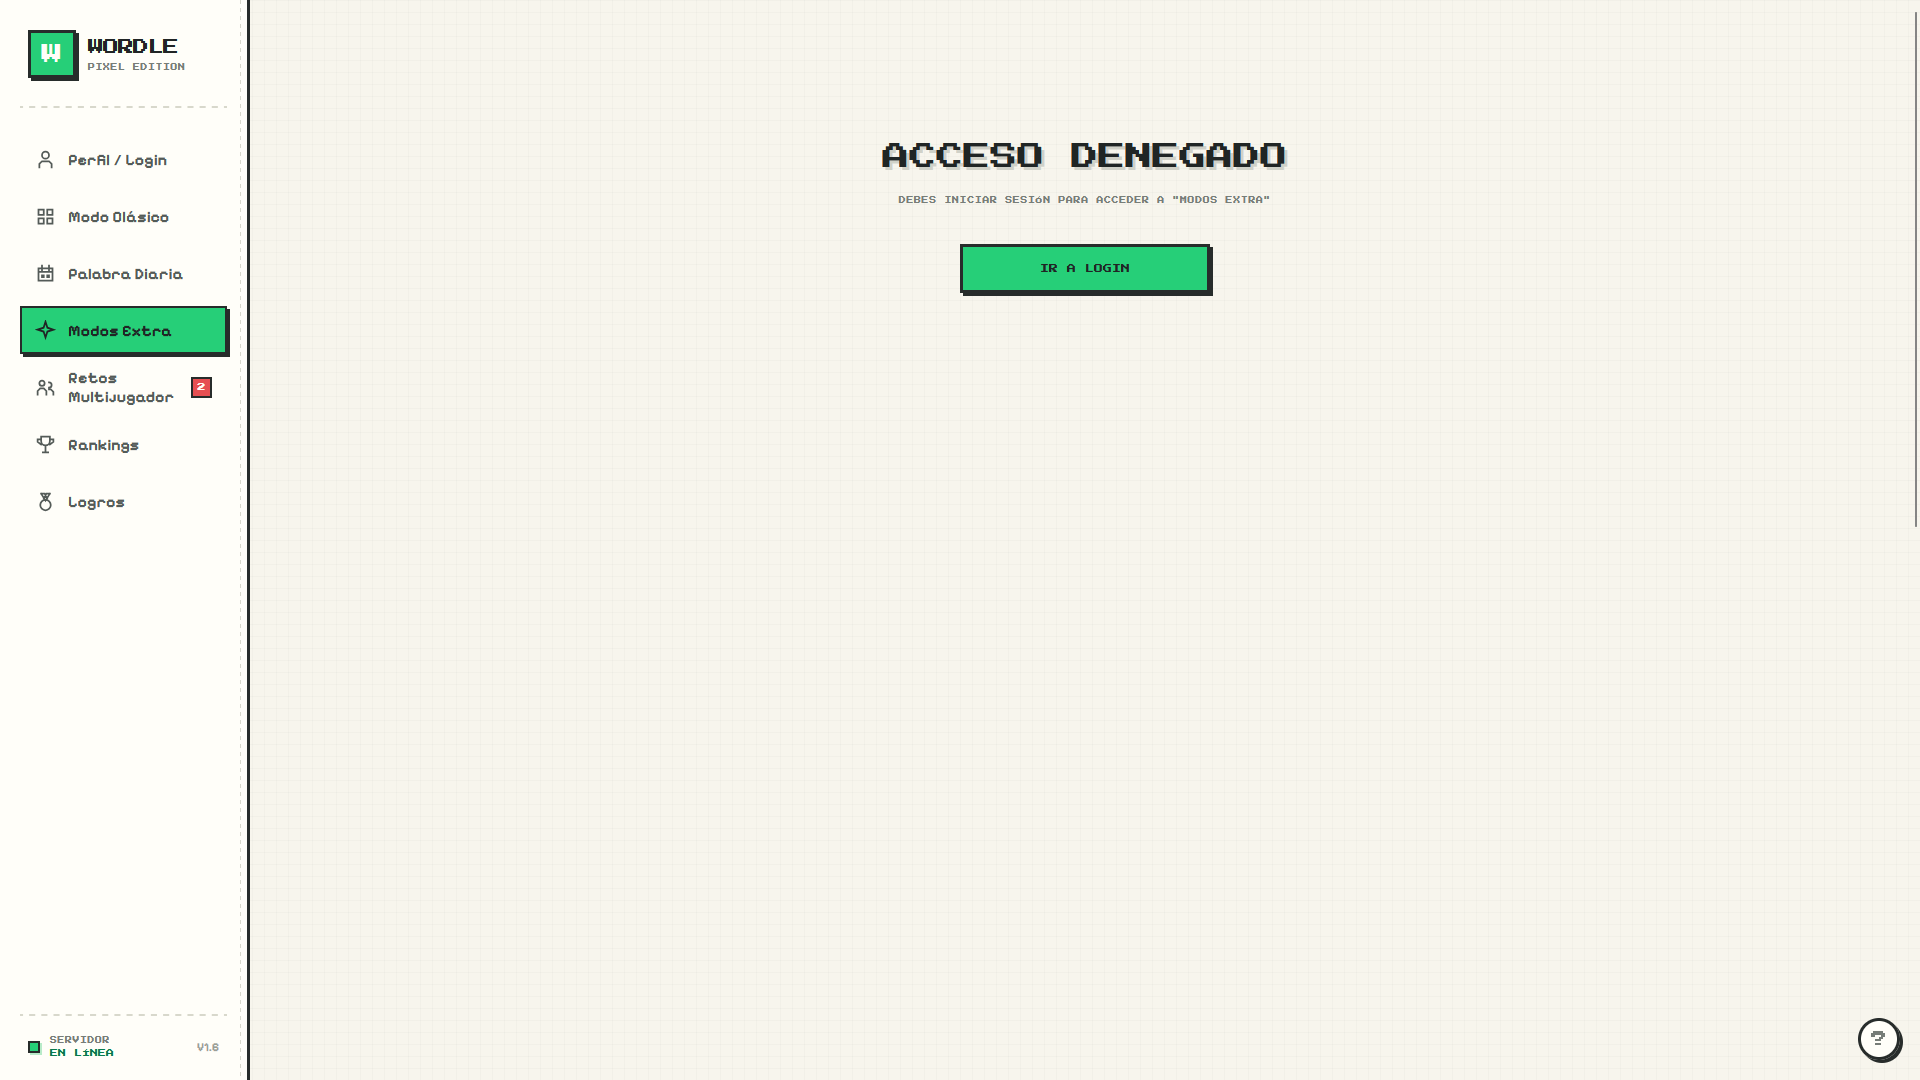
\includegraphics[width=0.85\linewidth]{Modos extra denied.png}}
  \caption{La opción "Modos extra" no disponible para invitado}
  \label{fig:modos-extra-denied-1}
\end{figure}}

% ------------------------- JUGAR 4 ------------------------------------------

\clearpage

\casoDeUso{\cduGraficoFuncDos}
  {Jugar 4}
  {El usuario registrado es capaz de seleccionar la pestaña del modo "jugar 4". Además, tiene el poder de escribir palabras y de enviarlas para poder terminar la partida. En caso de jugar se almacenará el resultado obtenido, incluyendo la fecha, si se ha resuelto correctamente y el número de intentos utilizados.}
  {Usuario.}
  {Estar identificado como usuario.}
  {Ninguno}
  {\begin{enumerate}
    \item El usuario entra a la página del juego y selecciona el modo de juego “jugar 4”.
    \item El usuario juega la partida (Ilustración 13).
    \item El usuario termina la partida:
    \begin{itemize}
      \item a. El usuario gana.
      \item b. El usuario pierde.
    \end{itemize}
  \end{enumerate}}
  {Se guarda la partida en el historial de juegos.}
  {\begin{figure}[H]
  \centering
  \fbox{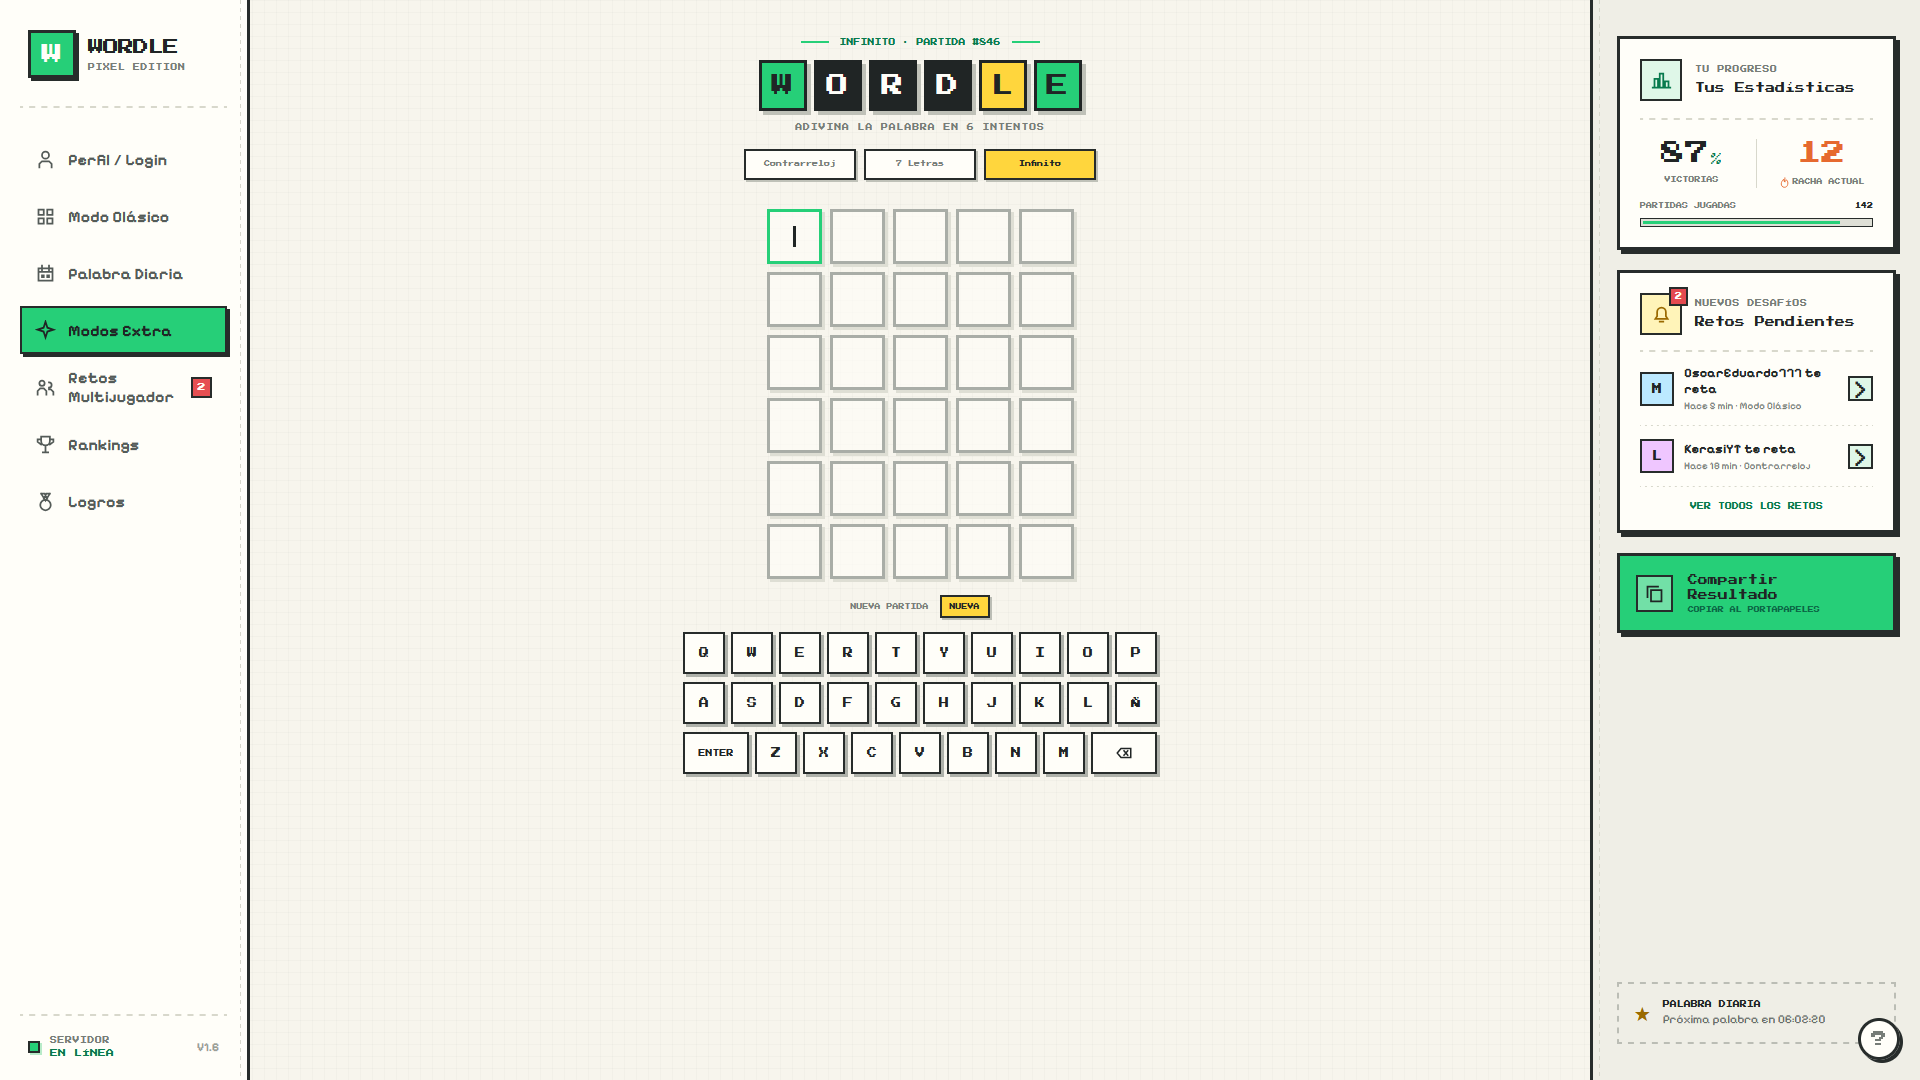
\includegraphics[width=0.85\linewidth]{Infinito.png}}
  \caption{Infinito}
  \label{fig:infinito}
\end{figure}
\begin{figure}[H]
  \centering
  \fbox{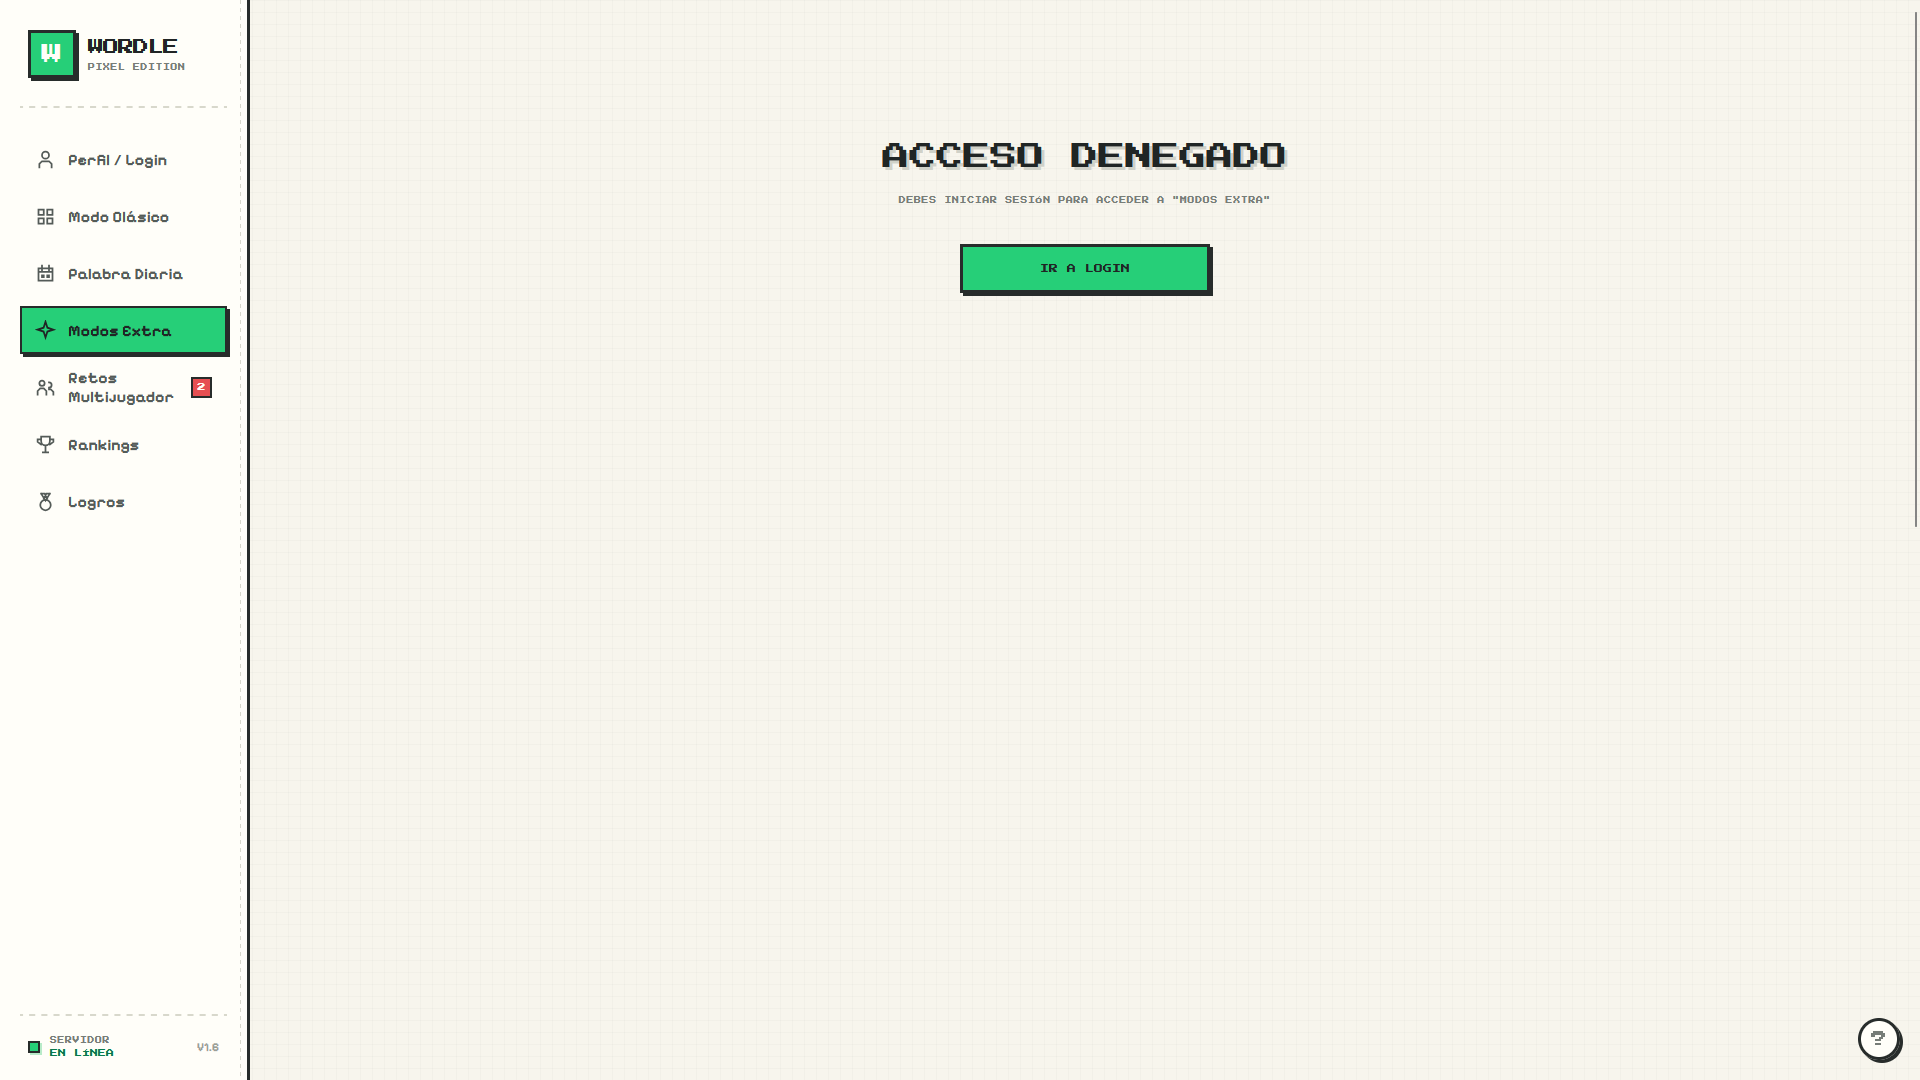
\includegraphics[width=0.85\linewidth]{Modos extra denied.png}}
  \caption{La opción "Modos extra" no disponible para invitado}
  \label{fig:modos-extra-denied-1}
\end{figure}}

% ===========================================================================
% FUNCIONALIDAD 3
% ===========================================================================
\clearpage
\funcionalidad{3}

\newcommand{\cduGraficoFuncTres}{%
  
\includegraphics[
    width=0.85\linewidth,
    height=4.5cm,
    keepaspectratio
  ]{Funcionalidad3.drawio.png}%
}



\casoDeUso{\cduGraficoFuncTres}
  {Palabra diaria}
  {Permite al usuario identificado entrar a la pestaña relacionada, entrando directamente a la pantalla del juego diario. Dando la posibilidad al usuario tanto de jugar como de consultar el histórico de sus resultados. En caso de jugar se almacenará el resultado obtenido, incluyendo la fecha, si se ha resuelto correctamente y el número de intentos utilizados.}
  {Usuario identificado}
  {No hay}
  {}
  {\begin{enumerate}
    \item El usuario selecciona en su menú principal “Juego Diario” (Ilustración 15) entrando directamente a la pantalla de juego y pudiendo acceder a la pestaña para el histórico de resultados.
    \item En caso de decidir acceder al histórico pulsando sobre la pestaña podrá acceder a los resultados.
    \item En caso de decidir jugar:
    \begin{itemize}
      \item a. Si ya ha jugado al juego de hoy le aparecerá la palabra diaria resuelta.
      \item b. Si no ha jugado dispondrá de una serie de intentos para acertar la palabra.
    \end{itemize}
  \end{enumerate}}
  {Se guardan los registros al terminar la partida. Guardar el progreso (cada palabra introducida).}
{\begin{figure}[H]
  \centering
  \fbox{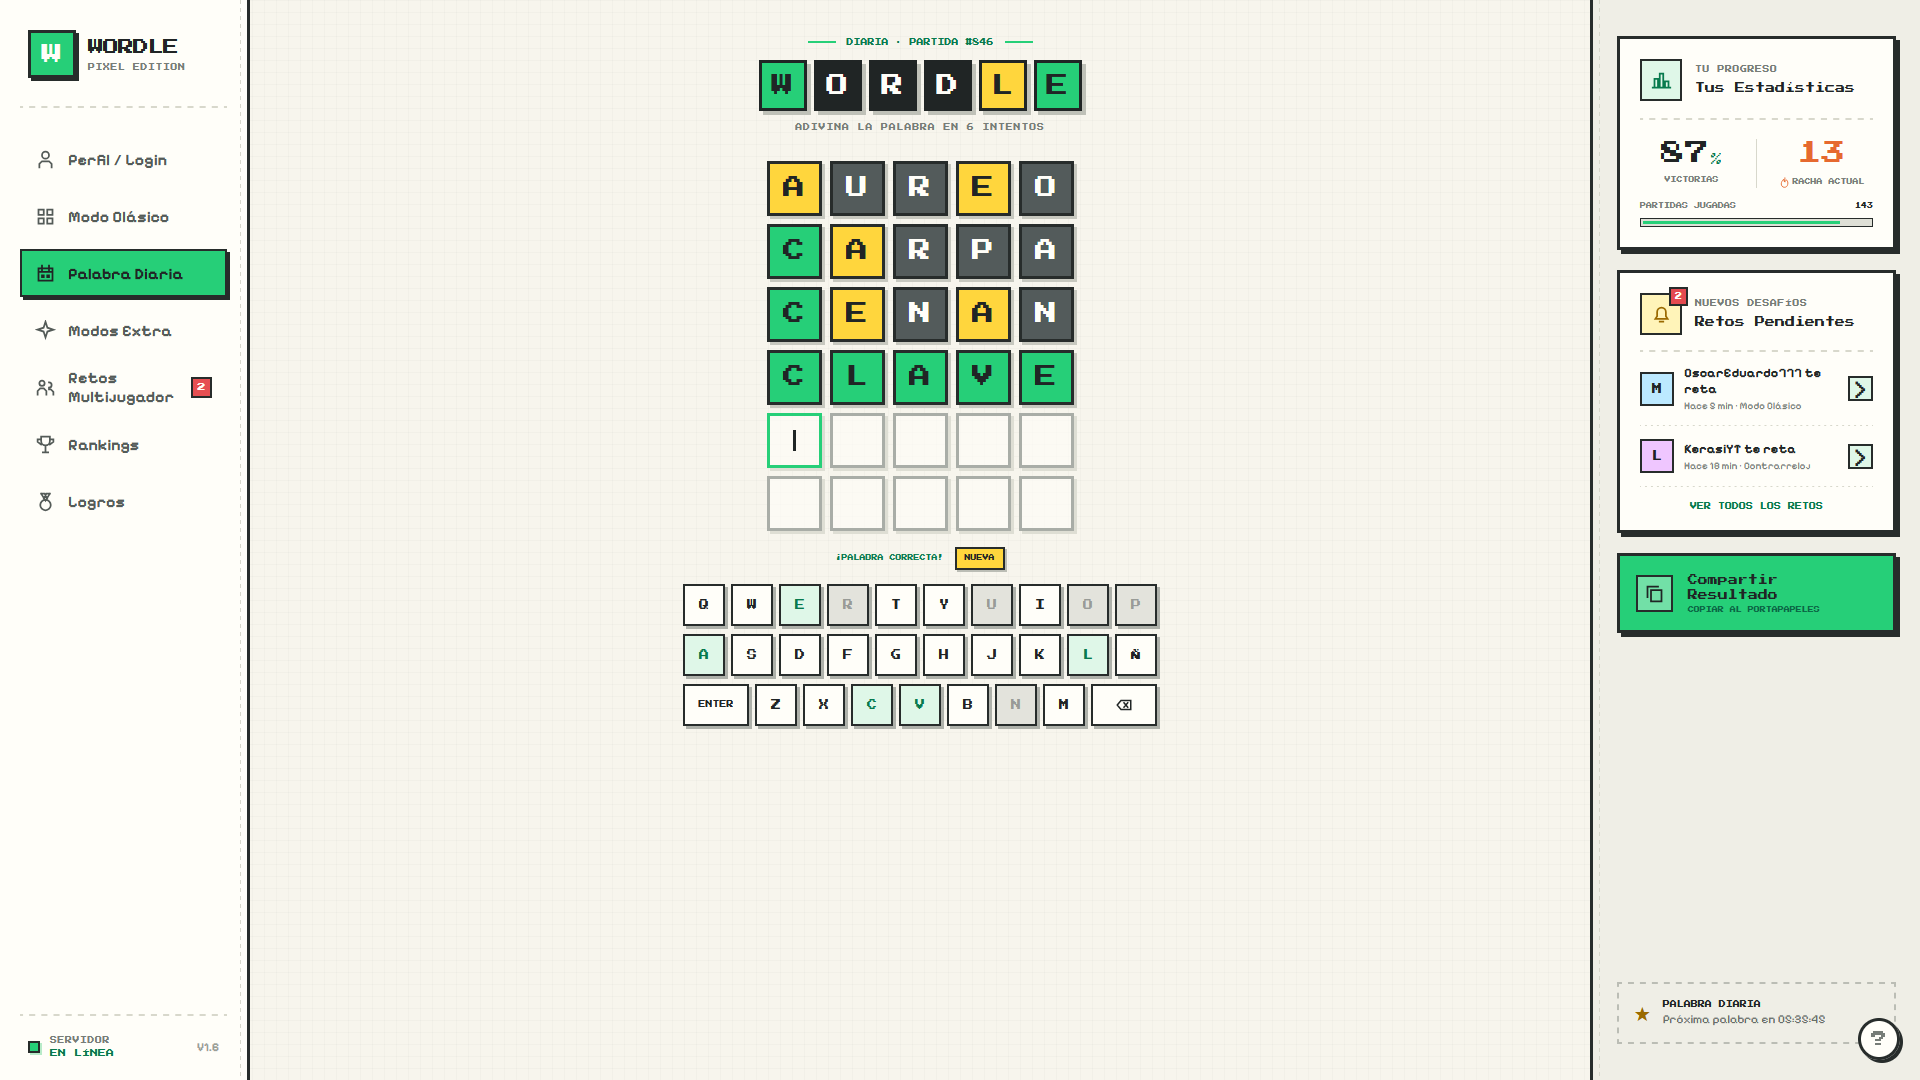
\includegraphics[width=0.85\linewidth]{Palabra diaria.png}}
  \caption{Palabra diaria}
  \label{fig:palabra-diaria}
\end{figure}
\begin{figure}[H]
  \centering
  \fbox{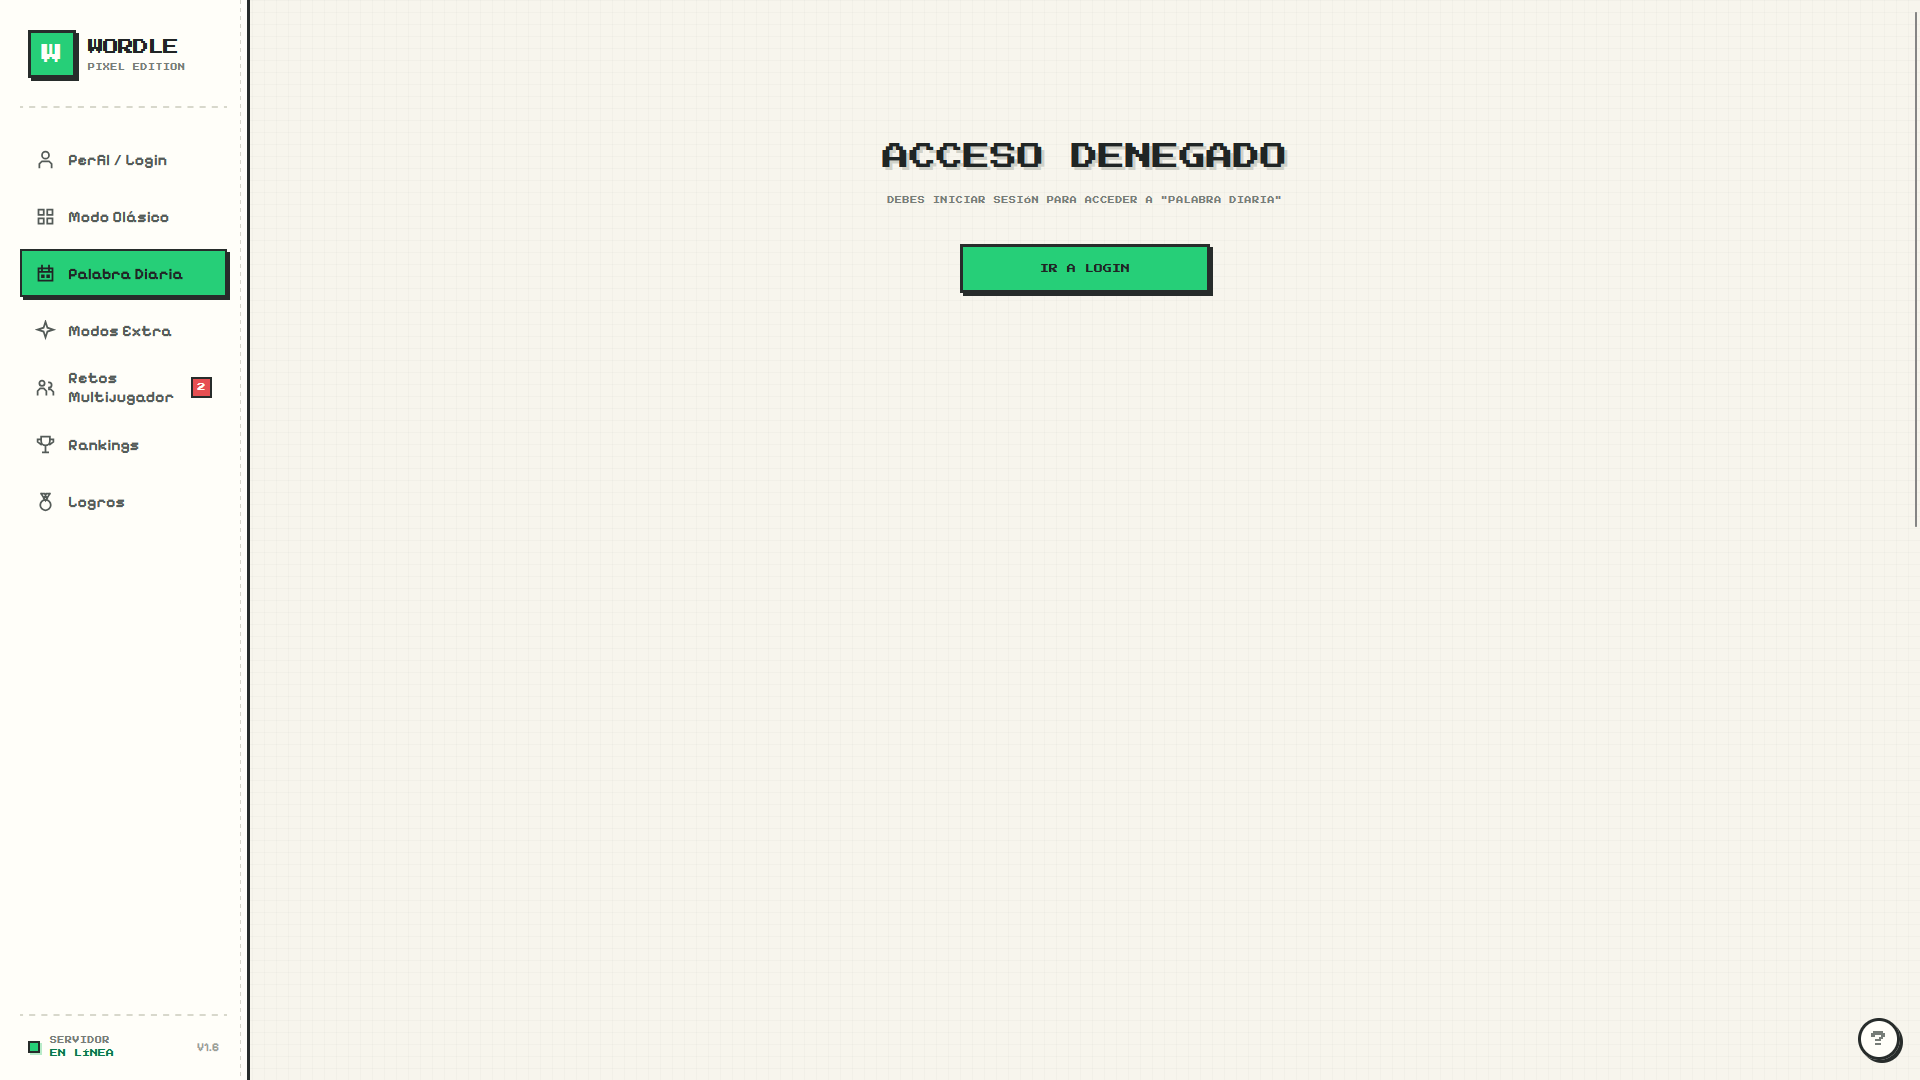
\includegraphics[width=0.85\linewidth]{Palabra diaria denied.png}}
  \caption{Palabra diaria no disponible para invitado}
  \label{fig:palabra-diaria-denied}
\end{figure}}

% ===========================================================================
% FUNCIONALIDAD 4
% ===========================================================================
\clearpage
\funcionalidad{4}

\newcommand{\cduGraficoFuncCuatro}{%
  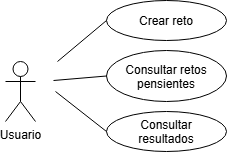
\includegraphics[
    width=0.9\linewidth,
    height=5.2cm,
    keepaspectratio
  ]{Funcionalidad4.png}%
}



\casoDeUso{\cduGraficoFuncCuatro}
  {Crear reto}
  {Permite a un usuario crear un reto dirigido a otro usuario especificando: usuario destinatario, palabra a resolver, número máximo de intentos y fecha límite.}
  {Usuario}
  {\begin{itemize}
    \item El usuario debe estar identificado.
    \item El destinatario debe existir.
  \end{itemize}}
  {\begin{itemize}
    \item La palabra a resolver debe almacenarse de forma cifrada en la base de datos para evitar su lectura antes de la finalización del reto. 
    \item El envío de la notificación al destinatario debe ser en tiempo real o entregarse en un tiempo máximo de 5 segundos tras registrar el reto. 
    \item El formulario debe validar en el cliente los límites del número de intentos y el formato de la fecha límite antes de enviar la petición al servidor. 

  \end{itemize}}
  {\begin{enumerate}
    \item Selecciona la opción “Crear reto”.
    \item El sistema muestra el formulario para crear el reto (Ilustración 17).
    \item El usuario introduce los datos:
    \begin{itemize}
      \item Destinatario
      \item Palabra
      \item Número máximo de intentos
      \item Fecha límite
    \end{itemize}
    \item El usuario confirma.
    \item El sistema valida los datos.
    \item El sistema registra el reto como “Pendiente”.
    \item El sistema notifica al destinatario.
    \item El sistema confirma la creación.
  \end{enumerate}}
  {\begin{itemize}
    \item El reto queda almacenado en “Retos pendientes”.
    \item El destinatario recibe una notificación.
  \end{itemize}}
{\begin{figure}[H]
  \centering
  \fbox{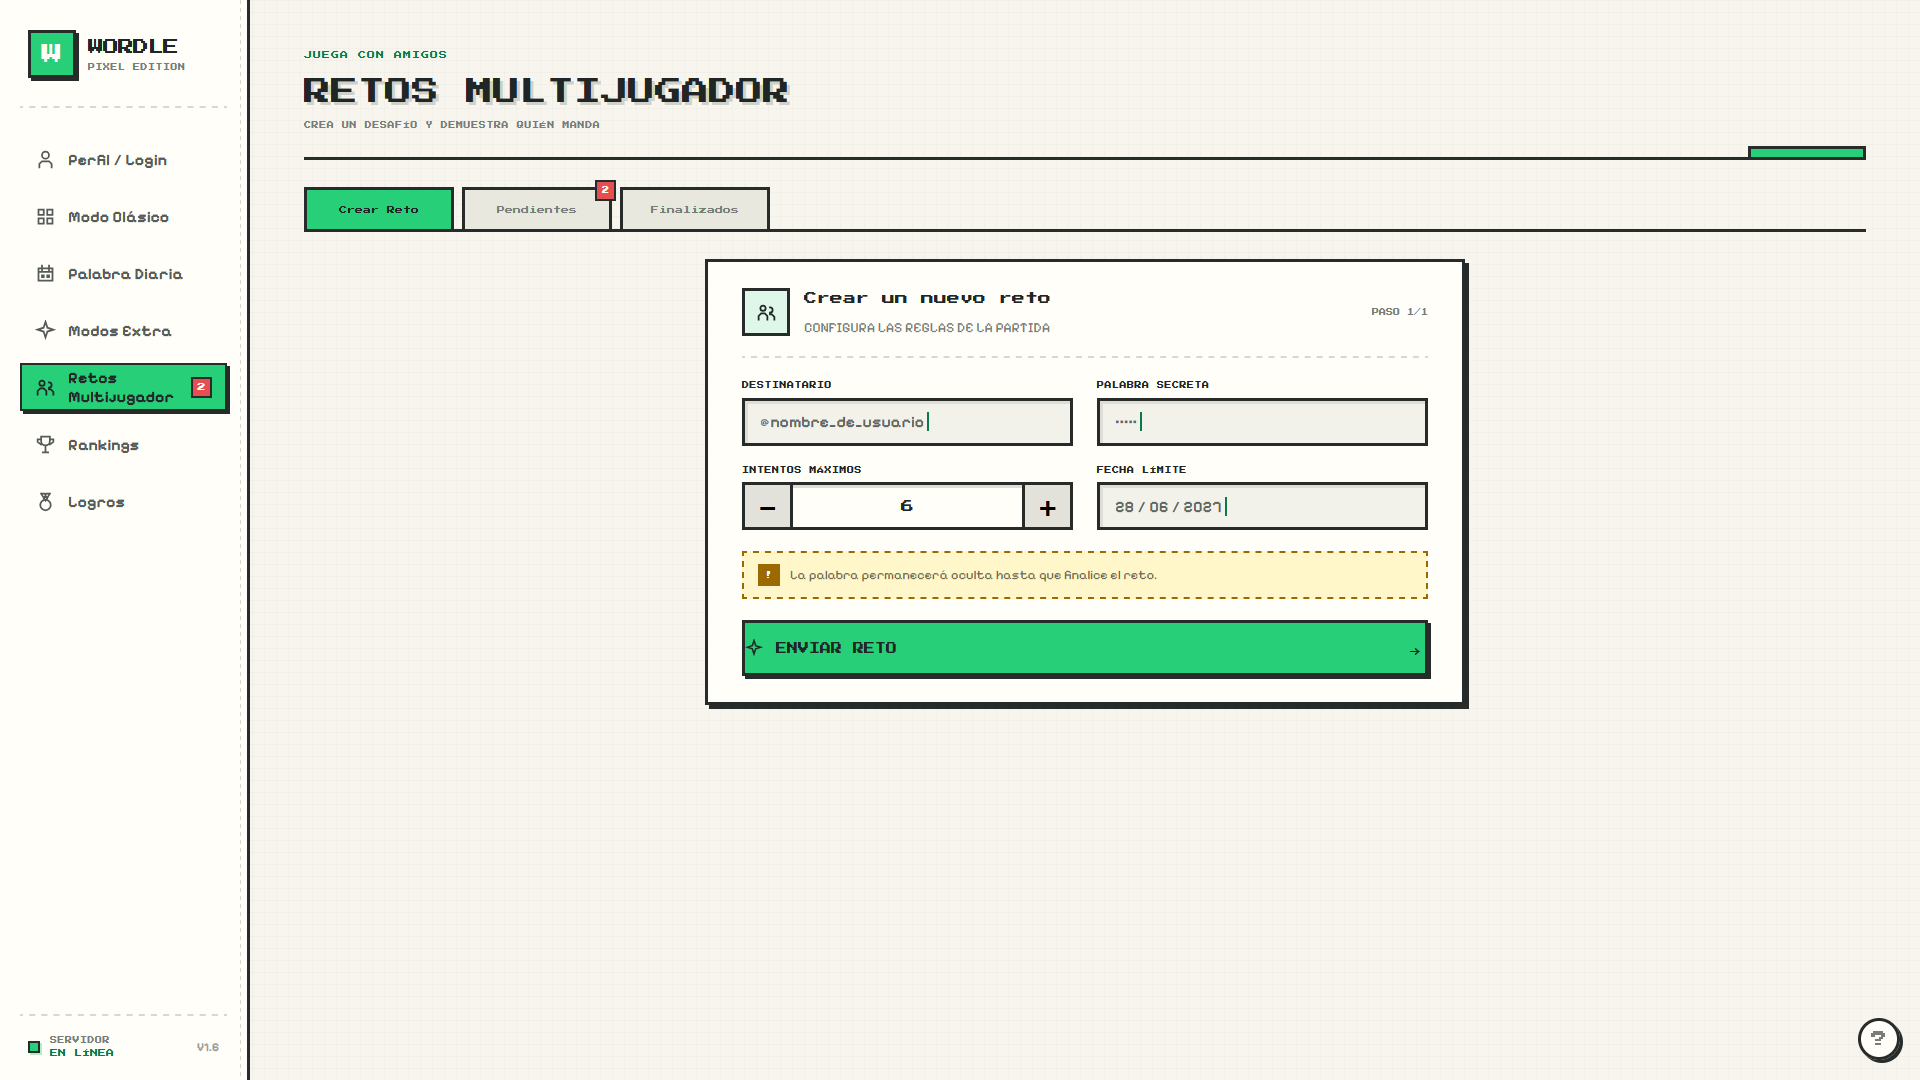
\includegraphics[width=0.85\linewidth]{Retos multijugador.png}}
  \caption{Retos multijugador}
  \label{fig:retos-multijugador}
\end{figure}
\begin{figure}[H]
  \centering
  \fbox{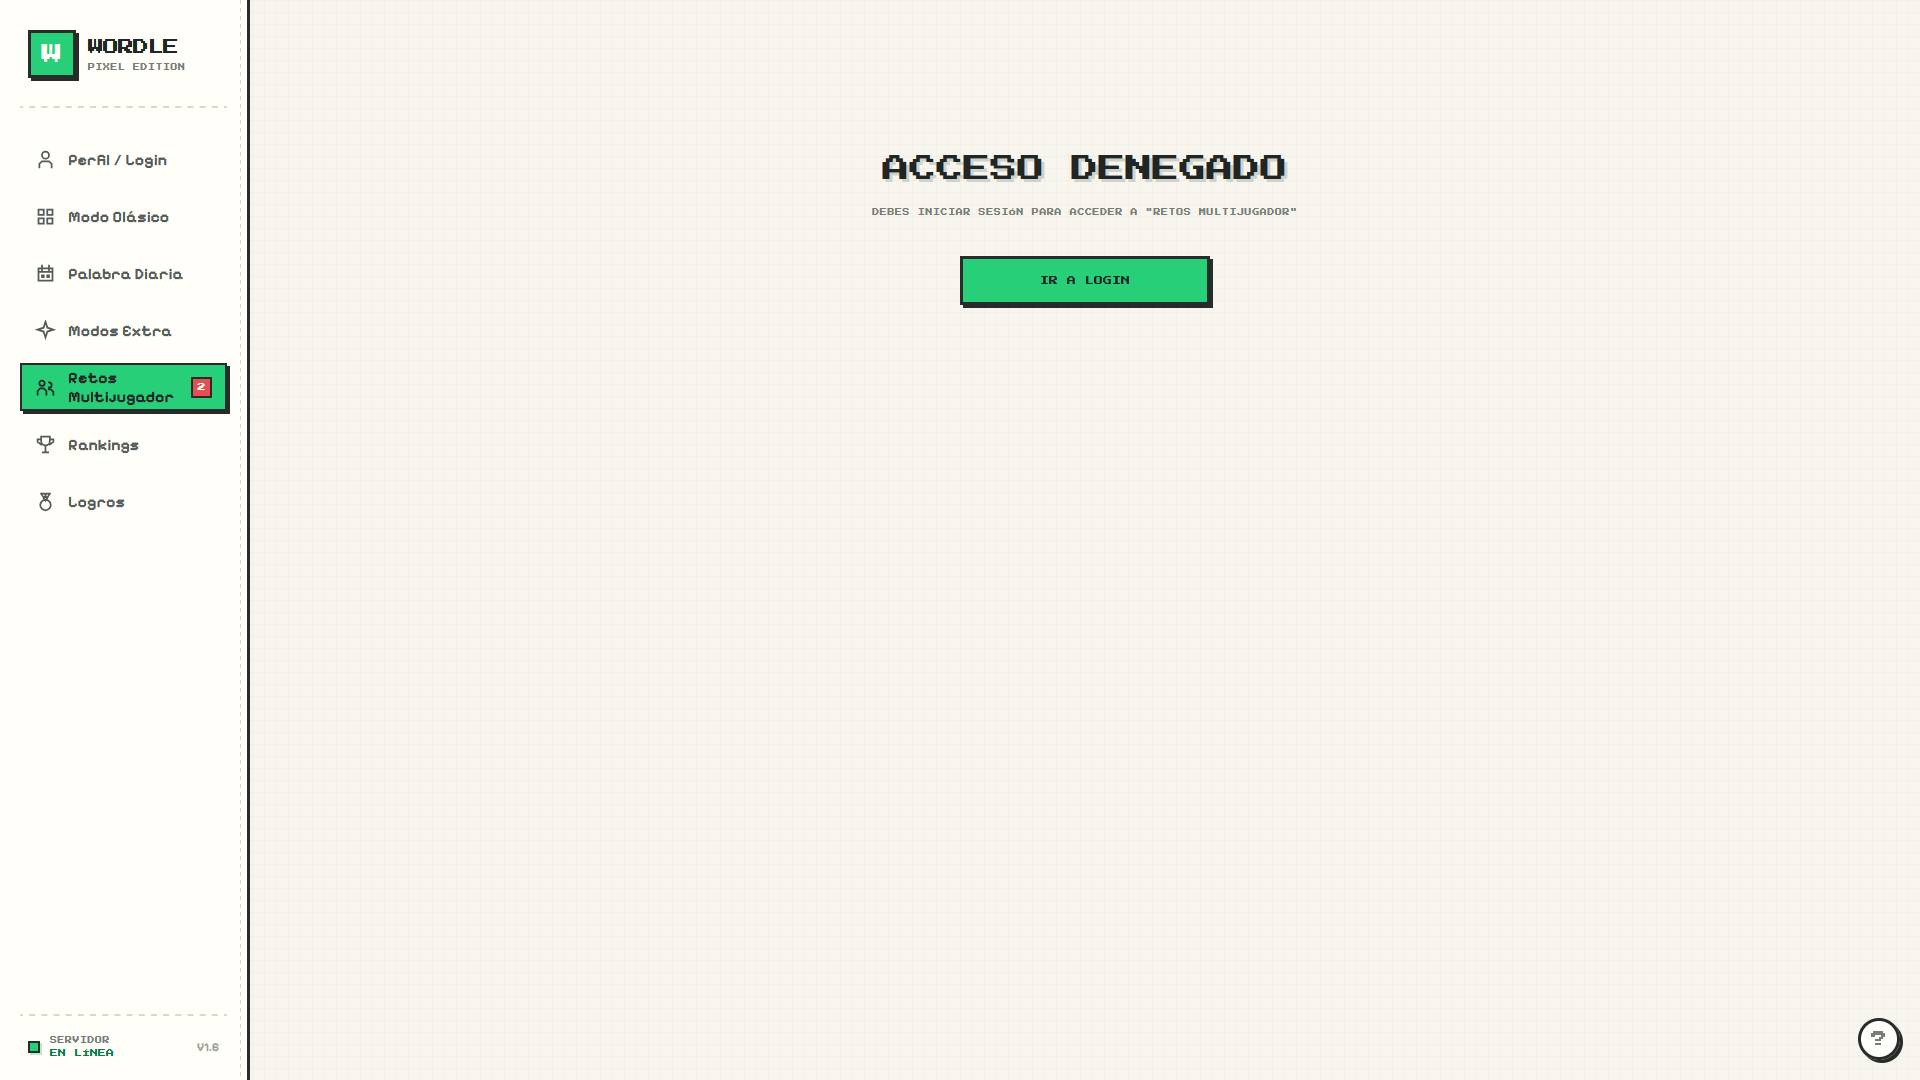
\includegraphics[width=0.85\linewidth]{Retos denied.png}}
  \caption{Retos no disponibles para invitado}
  \label{fig:retos-denied}
\end{figure}}

\clearpage

\casoDeUso{\cduGraficoFuncCuatro}
  {Consultar retos pendientes}
  {Permite visualizar todos los retos recibidos que todavía no han sido jugados ni han caducado. Se da además la opción de aceptar o rechazar dicho reto.}
  {Usuario}
  {El usuario debe estar identificado.}
  {\begin{itemize}
    \item El tiempo de carga y visualización de la lista de retos pendientes no debe exceder de 1,5 segundos. 
    \item El listado debe actualizarse automáticamente excluyendo de forma inmediata los retos que hayan caducado según su fecha límite. 
    \item La interfaz debe mostrar el listado de retos formateado adecuadamente en cualquier dispositivo móvil o de escritorio de forma clara y accesible. 
    \item En caso de haber más de 20 retos pendientes, la interfaz debe implementar paginación para no ralentizar la aplicación. 
  \end{itemize}}
  {\begin{enumerate}
    \item El usuario accede a "Pendientes" (Ilustración 19).
    \item El sistema recupera los retos pendientes.
    \item El sistema muestra el listado (Ilustración 19).
    \item El usuario selecciona un reto para ver detalles.
  \end{enumerate}}
  {No hay}
{\begin{figure}[H]
  \centering
  \fbox{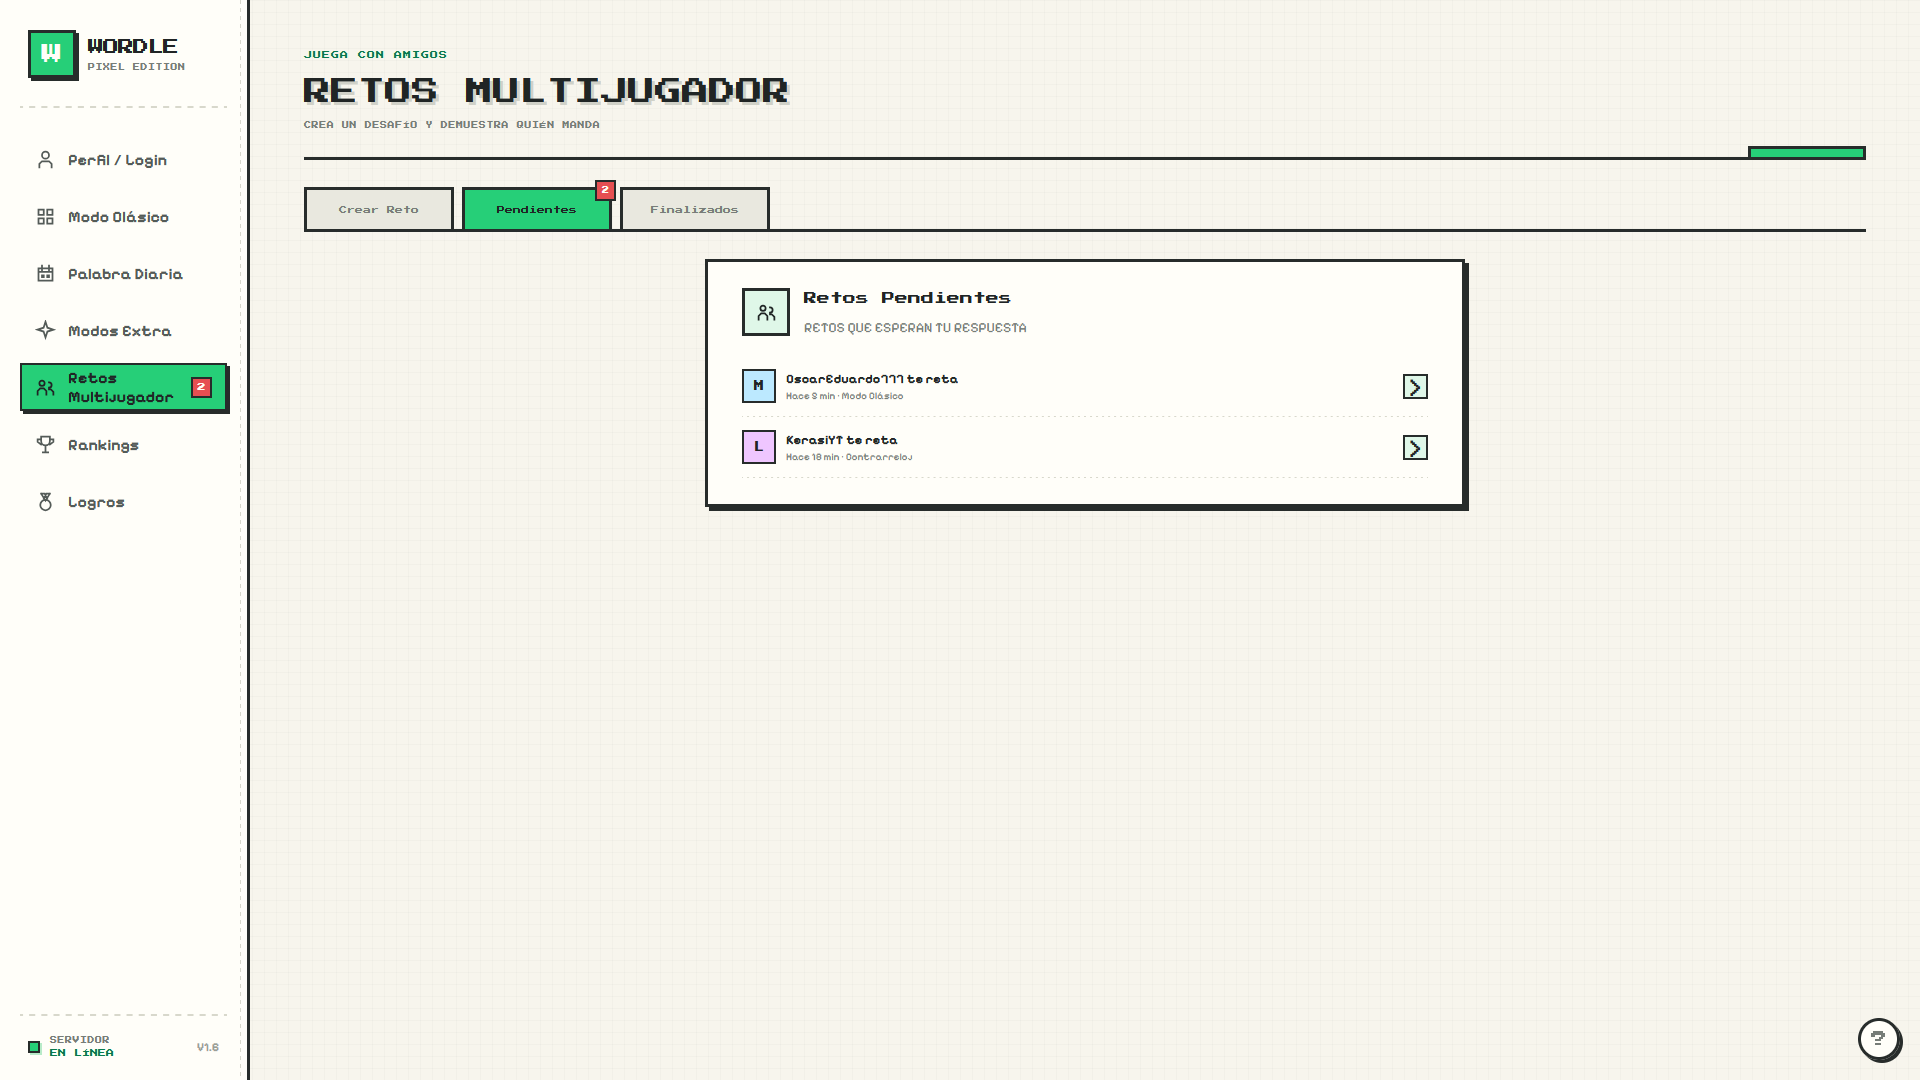
\includegraphics[width=0.85\linewidth]{Retos pendientes.png}}
  \caption{Retos pendientes}
  \label{fig:retos-pendientes}
\end{figure}}

\clearpage

\casoDeUso{\cduGraficoFuncCuatro}
  {Consultar resultados}
  {Permite visualizar los resultados de los retos ya finalizados.}
  {Usuario}
  {El usuario debe estar identificado.}
  {\begin{itemize}
      \item Solo el usuario autenticado que participó en el reto (creador o destinatario) puede consultar la información del resultado. 
  \end{itemize}}
  {\begin{enumerate}
    \item El usuario accede a "Finalizados" (Ilustración 20).
    \item Selecciona un reto.
    \item El sistema recupera los datos del resultado.
    \item El sistema muestra:
    \begin{itemize}
      \item ganador/perdedor.
      \item intentos utilizados.
      \item fecha de finalización.
    \end{itemize}
  \end{enumerate}}
  {No hay}
{\begin{figure}[H]
  \centering
  \fbox{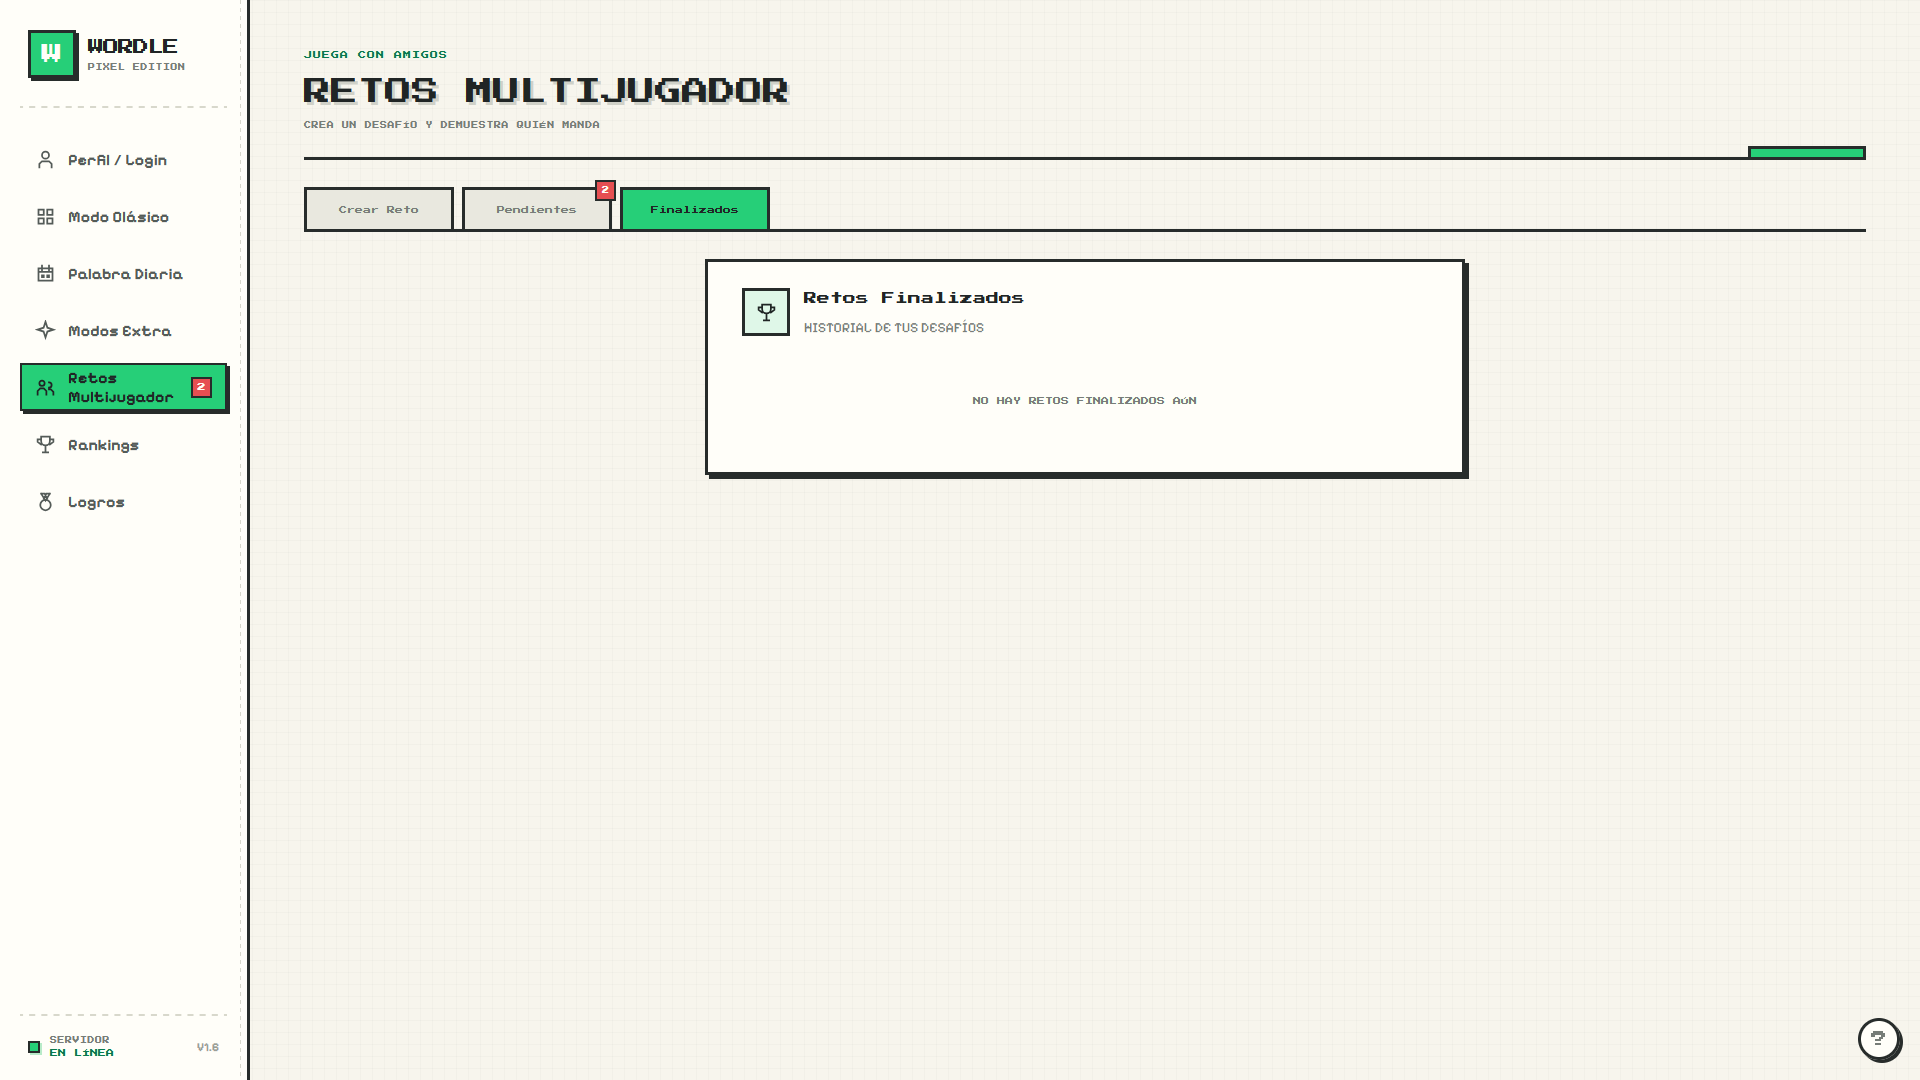
\includegraphics[width=0.85\linewidth]{Retos finalizados.png}}
  \caption{Retos finalizados}
  \label{fig:retos-finalizados}
\end{figure}}

% ===========================================================================
% FUNCIONALIDAD 5
% ===========================================================================
\clearpage
\funcionalidad{5}

\newcommand{\cduGraficoFuncCinco}{%
  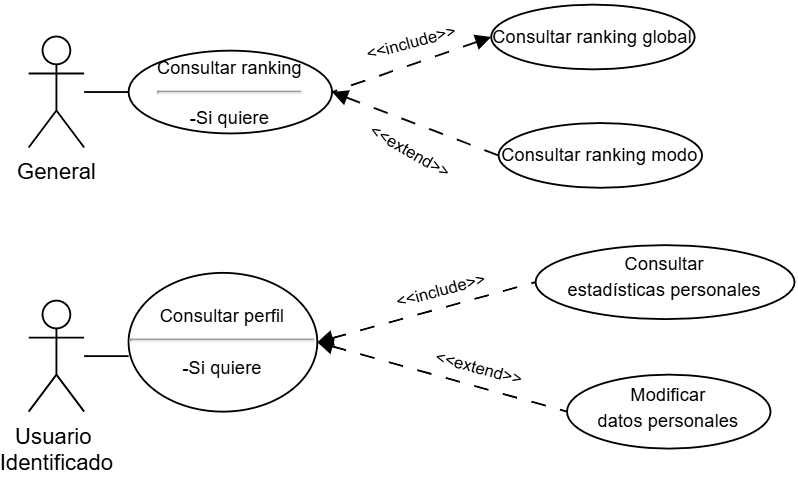
\includegraphics[
    width=0.9\linewidth,
    height=5.2cm,
    keepaspectratio
  ]{Funcianalidad5.png}%
}



\casoDeUso{\cduGraficoFuncCinco}
  {Consultar ranking}
  {Permite a los usuarios (tanto registrados como invitados) entrar en la pestaña de rankings para acceder a las distintas clasificaciones disponibles.}
  {Usuario registrado, invitado}
  {Ninguna.}
  {\begin{itemize}
    \item El sistema debe soportar la conexión y el acceso simultáneo de al menos 1000 usuarios (tanto registrados como invitados) a la pestaña principal de rankings sin experimentar caídas de servicio.
    \item El tiempo de carga para mostrar la pantalla principal con las opciones de clasificación debe ser inferior a 2 segundos.
  \end{itemize}}
  {\begin{enumerate}
    \item El usuario selecciona la pestaña de "Rankings" (Ilustración 21).
    \item El sistema muestra la pantalla principal de clasificaciones, ofreciendo las opciones de ver rankings globales o por modo de juego.
  \end{enumerate}}
  {}
{\begin{figure}[H]
  \centering
  \fbox{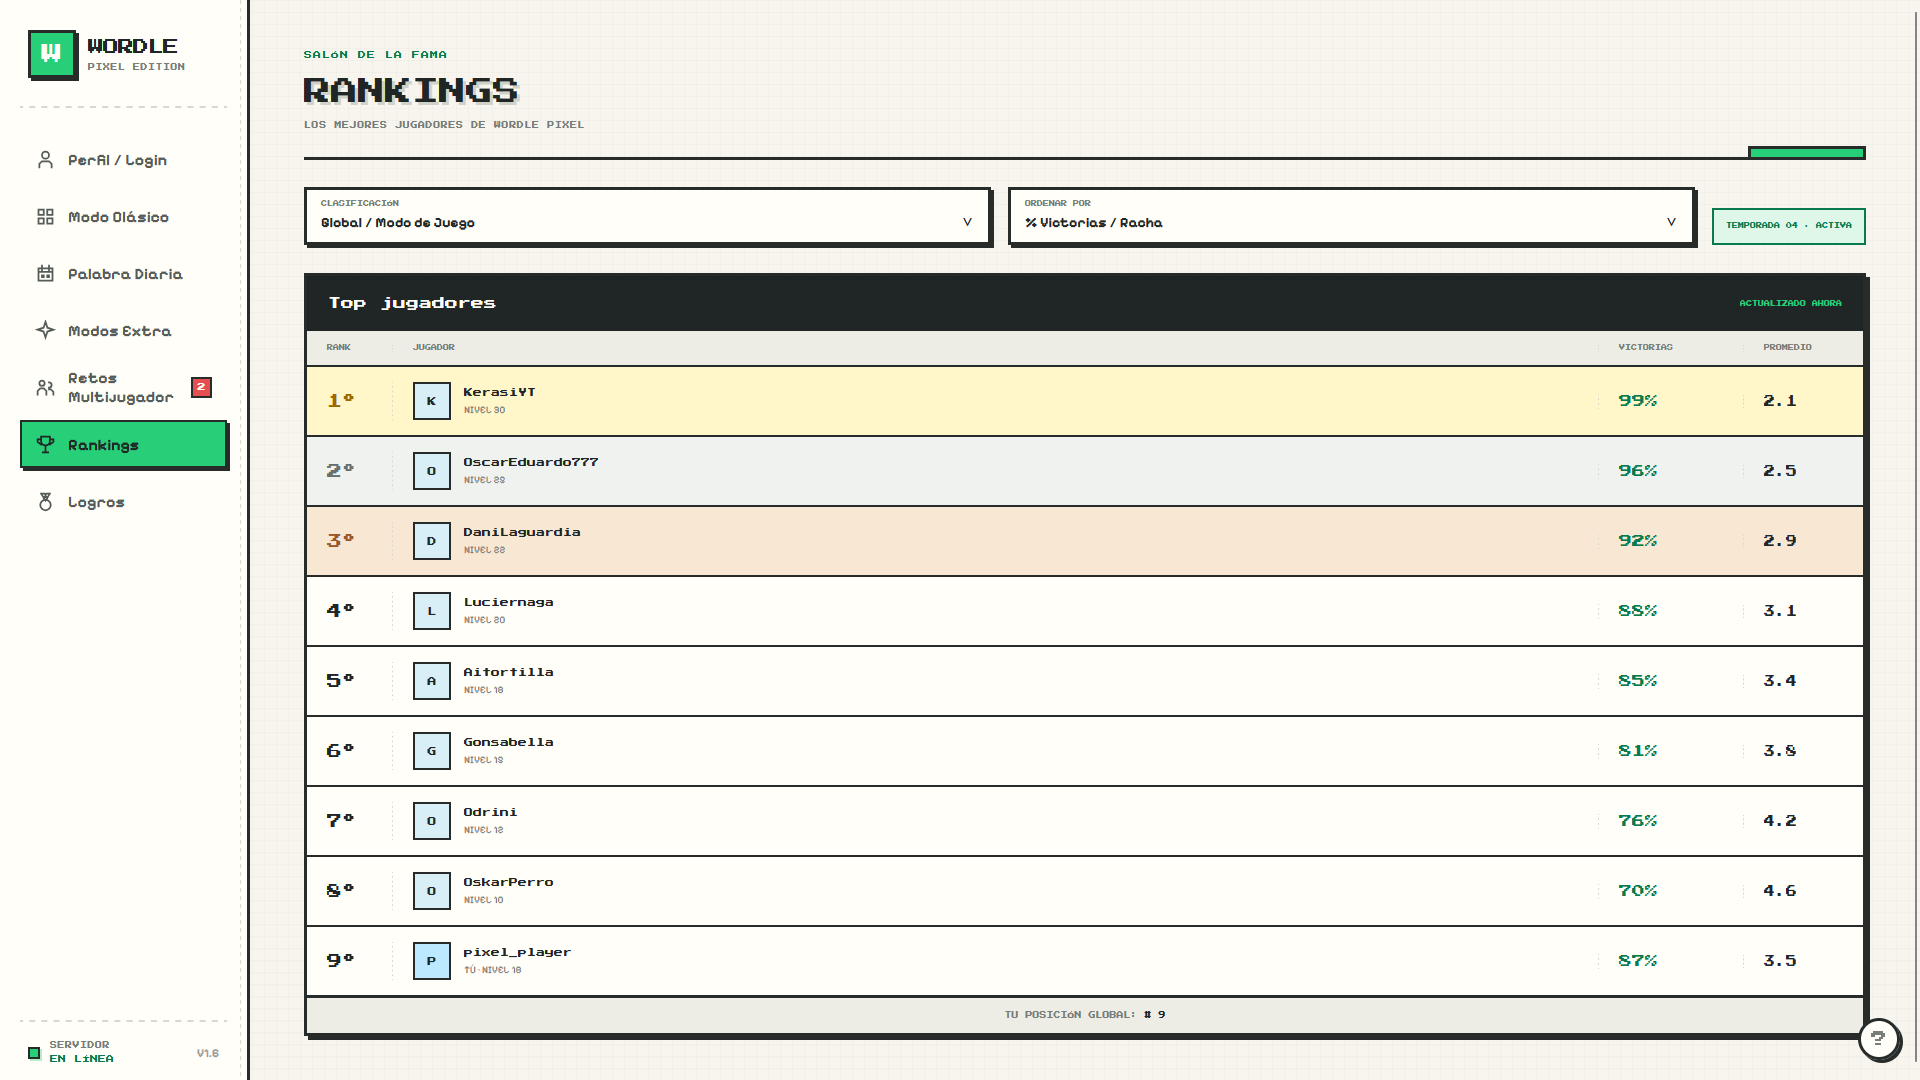
\includegraphics[width=0.85\linewidth]{Ranking.png}}
  \caption{Ranking}
  \label{fig:ranking}
\end{figure}}

\clearpage

\casoDeUso{\cduGraficoFuncCinco}
  {Consultar ranking de manera global}
  {Permite a cualquier usuario (registrado o invitado) consultar la clasificación general de todos los jugadores del sistema basándose en el porcentaje de victorias, la racha máxima de victorias y el número medio de intentos empleados.}
  {Usuario registrado, invitado}
  {Ninguna.}
  {\begin{itemize}
    \item El sistema debe ser capaz de procesar hasta 500 consultas concurrentes de usuarios filtrando la clasificación general.
    \item La actualización de la lista de jugadores, basándose en el porcentaje de victorias, la racha máxima de victorias y el número medio de intentos empleados, debe reflejarse en tiempo real conforme finalizan las partidas.
    \item El tiempo de respuesta del sistema para ordenar y devolver los datos de todos los jugadores según el filtro seleccionado no debe superar los 3 segundos.
  \end{itemize}}
  {\begin{enumerate}
    \item El usuario selecciona la opción "Ranking Global".
    \item El usuario elige el filtro deseado: porcentaje de victorias, racha máxima o media de intentos.
    \item El sistema recupera los datos y muestra la lista ordenada de usuarios según el criterio elegido (Ilustración 22).
  \end{enumerate}}
  {El usuario visualiza la lista de clasificación global actualizada.}
{\begin{figure}[H]
  \centering
  \fbox{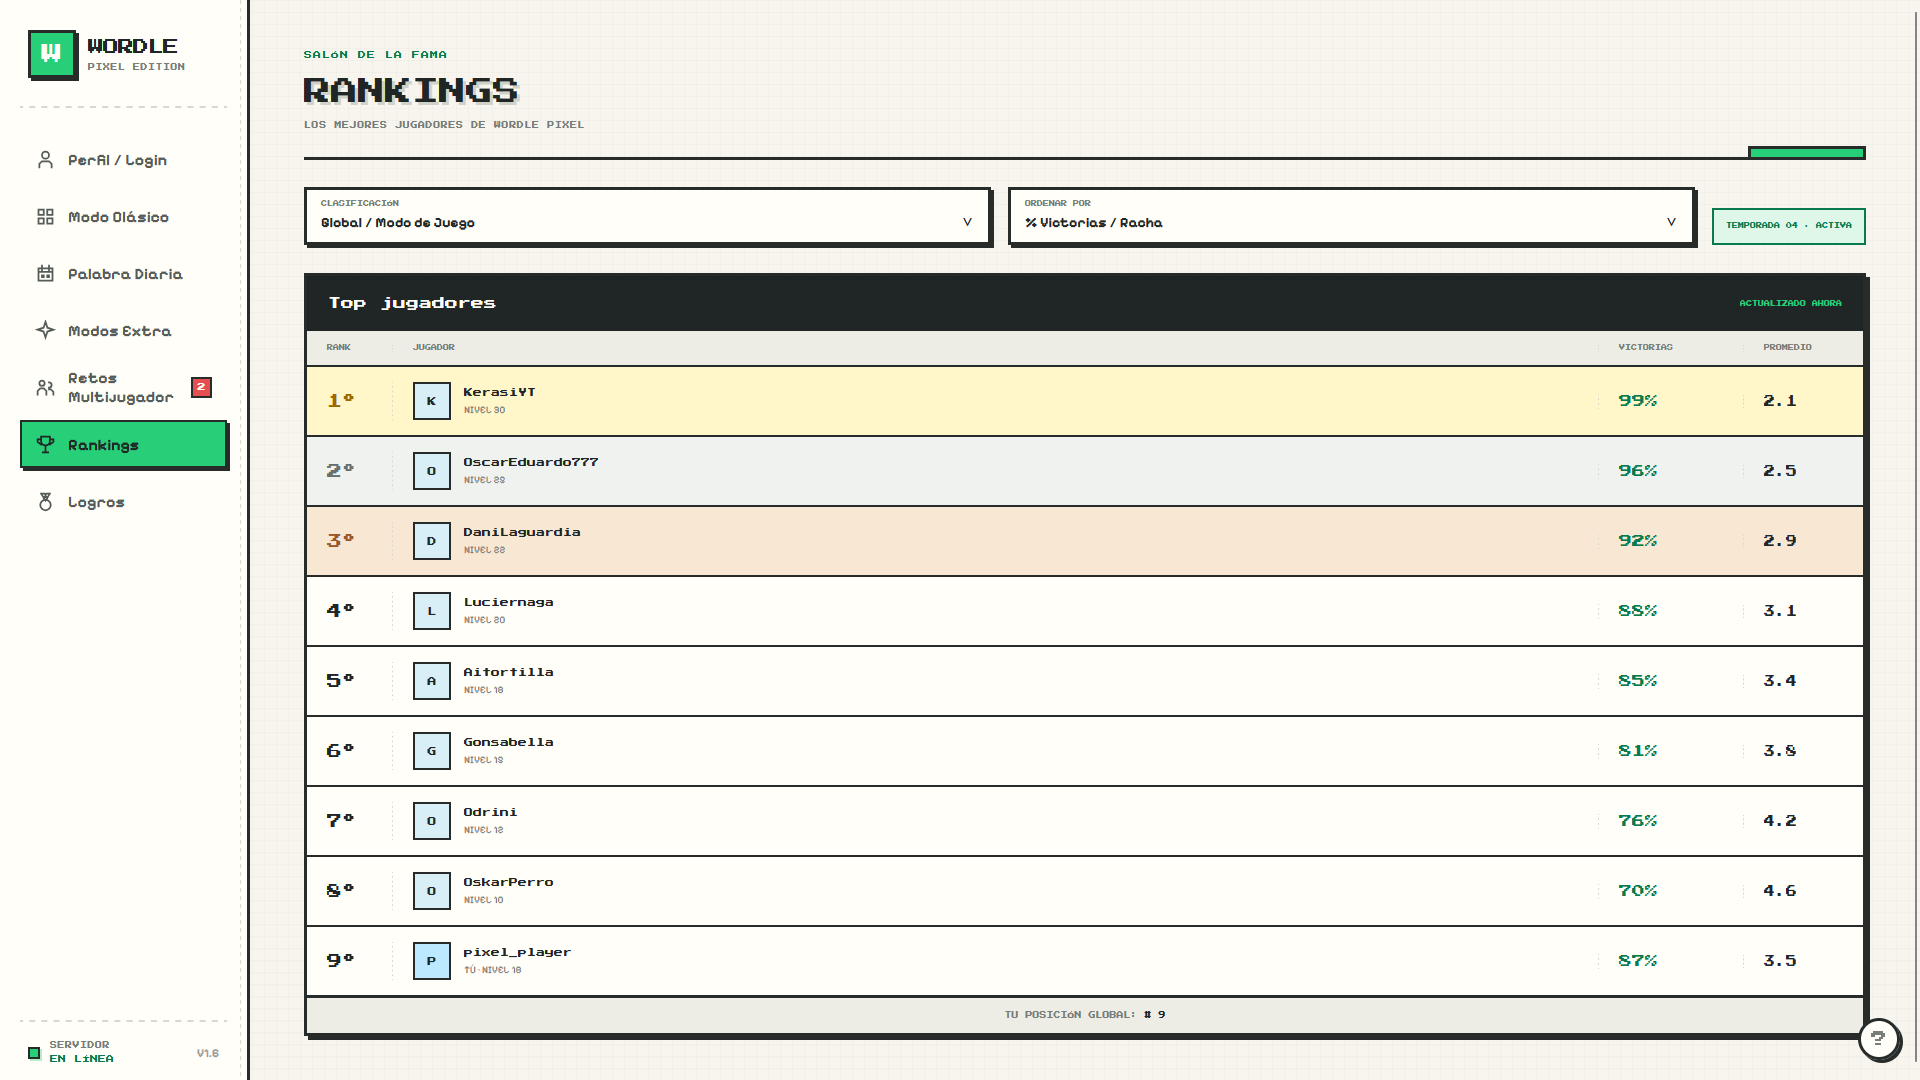
\includegraphics[width=0.85\linewidth]{Ranking.png}}
  \caption{Ranking global}
  \label{fig:ranking-global}
\end{figure}}

\clearpage

\casoDeUso{\cduGraficoFuncCinco}
  {Consultar ranking por modo de juego}
  {Permite a cualquier usuario (registrado o invitado) consultar la clasificación de los jugadores filtrada de manera específica para un modo de juego concreto.}
  {Usuario registrado, invitado}
  {Ninguna.}
  {\begin{itemize}
    \item Los datos de la clasificación filtrada por modos de juego deben actualizarse en tiempo real, garantizando la consistencia con las partidas recién terminadas en dicho modo.
    \item El cambio de filtro entre un modo de juego y otro (junto con su criterio de porcentaje, racha o intentos) debe aplicarse en la interfaz en menos de 1 segundo.
  \end{itemize}}
  {\begin{enumerate}
    \item El usuario selecciona la opción "Ranking por Modo de Juego".
    \item El sistema solicita seleccionar uno de los modos de juego disponibles.
    \item El usuario elige el modo de juego y el criterio de clasificación (porcentaje de victorias, racha máxima o media de intentos).
    \item El sistema muestra la lista ordenada correspondiente a ese modo específico (Ilustración 23).
  \end{enumerate}}
  {El usuario visualiza el ranking filtrado por el modo de juego seleccionado.}
{\begin{figure}[H]
  \centering
  \fbox{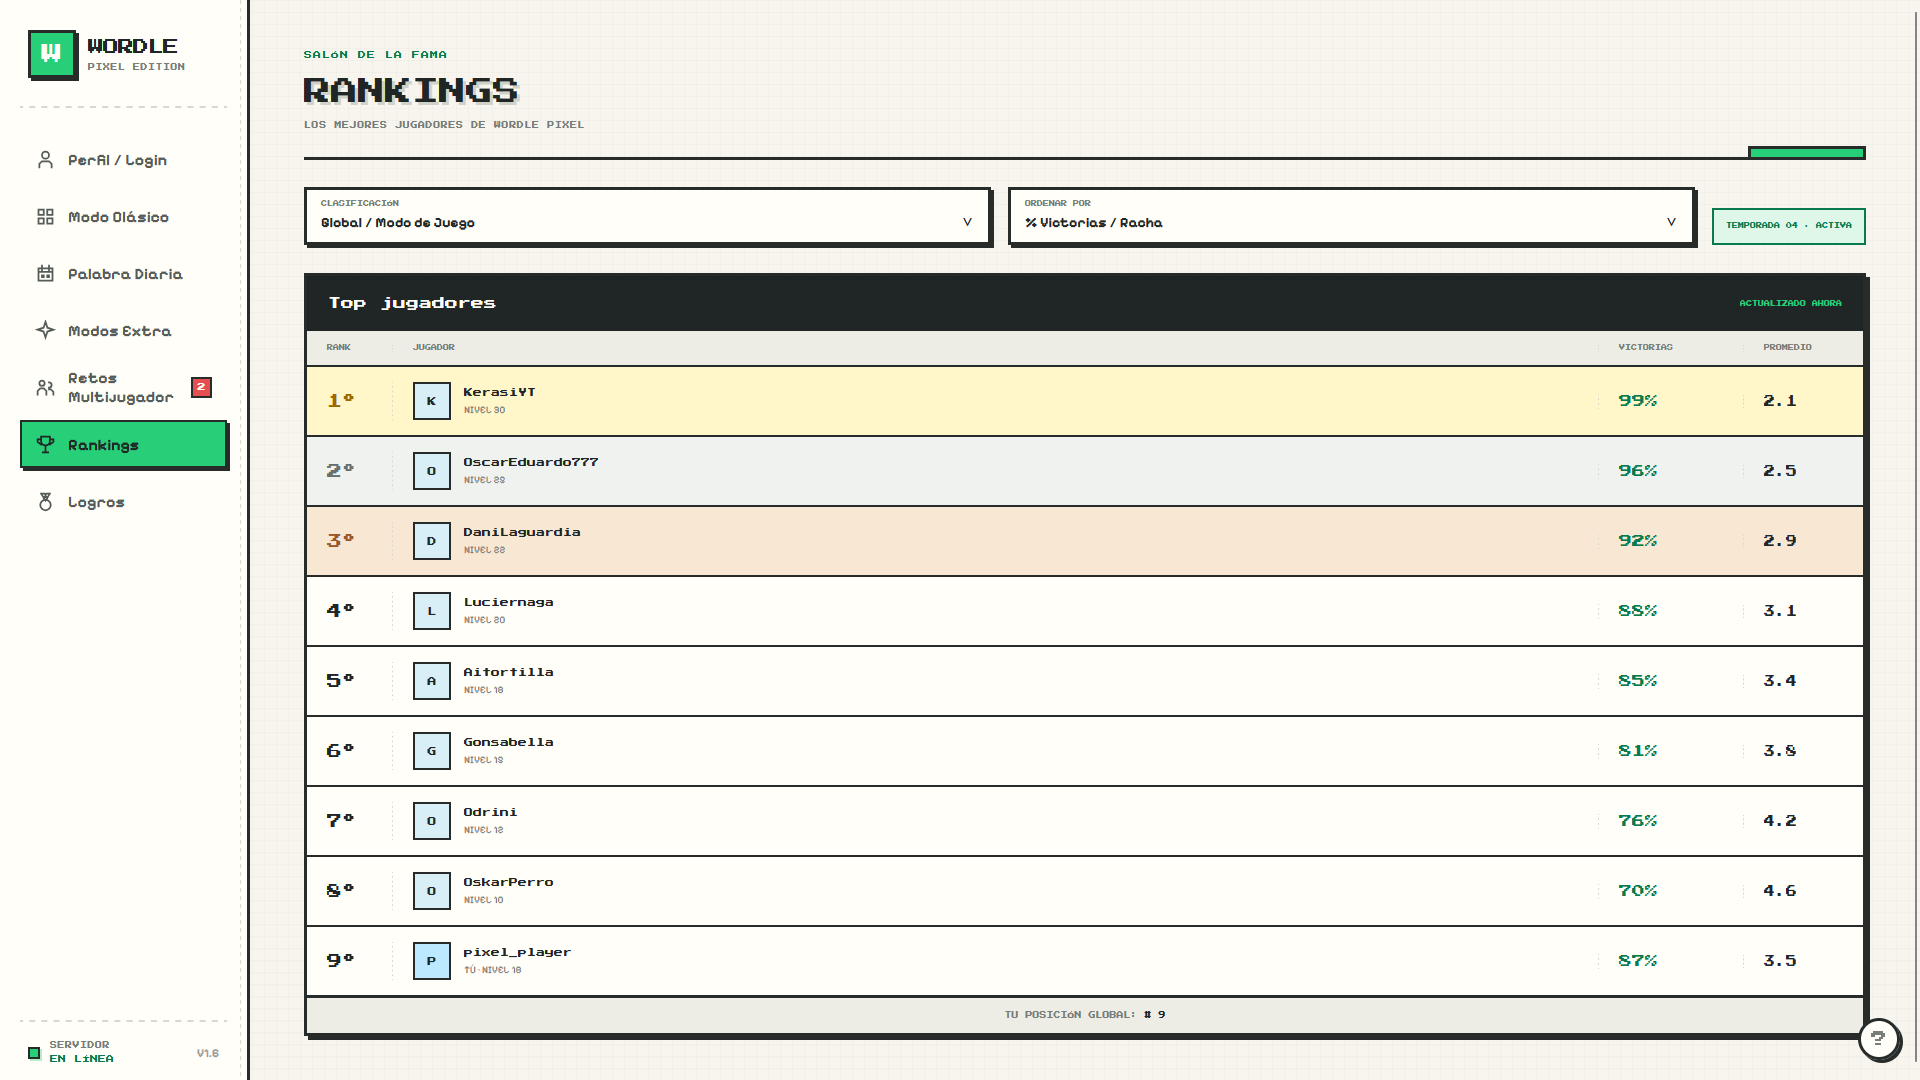
\includegraphics[width=0.85\linewidth]{Ranking.png}}
  \caption{Ranking por modo de juego}
  \label{fig:ranking-modo}
\end{figure}}

\clearpage

\casoDeUso{\cduGraficoFuncCinco}
  {Consultar estadísticas personales detalladas}
  {Permite a un usuario registrado consultar sus propias estadísticas detalladas generadas a partir de su historial de partidas. El usuario invitado no tiene acceso a esta opción al no disponer de estadísticas vinculadas.}
  {Usuario registrado}
  {El usuario debe estar registrado e identificado en el sistema.}
  {\begin{itemize}
    \item El sistema debe garantizar la privacidad y seguridad de los datos, validando el token de sesión en tiempo real.
    \item El sistema debe recuperar el historial completo de partidas del usuario para calcular los datos estadísticos en menos de 2 segundos.
    \item La disponibilidad de la base de datos del historial personal debe ser del 99.9\%.
  \end{itemize}}
  {\begin{enumerate}
    \item El usuario selecciona la opción "Mis estadísticas" (Ilustración 24).
    \item El sistema verifica la identidad del usuario.
    \item El sistema recupera el historial y muestra los datos personales (porcentaje de victorias, racha actual, racha máxima, intentos medios).
  \end{enumerate}

  \si{Qué pasa si...}

  \begin{itemize}
    \item A. El usuario es un invitado: El sistema oculta el botón de estadísticas personales o muestra un mensaje indicando que debe registrarse para almacenar y visualizar sus estadísticas.
  \end{itemize}}
  {El usuario visualiza su panel de estadísticas personales detalladas.}
{\begin{figure}[H]
  \centering
  \fbox{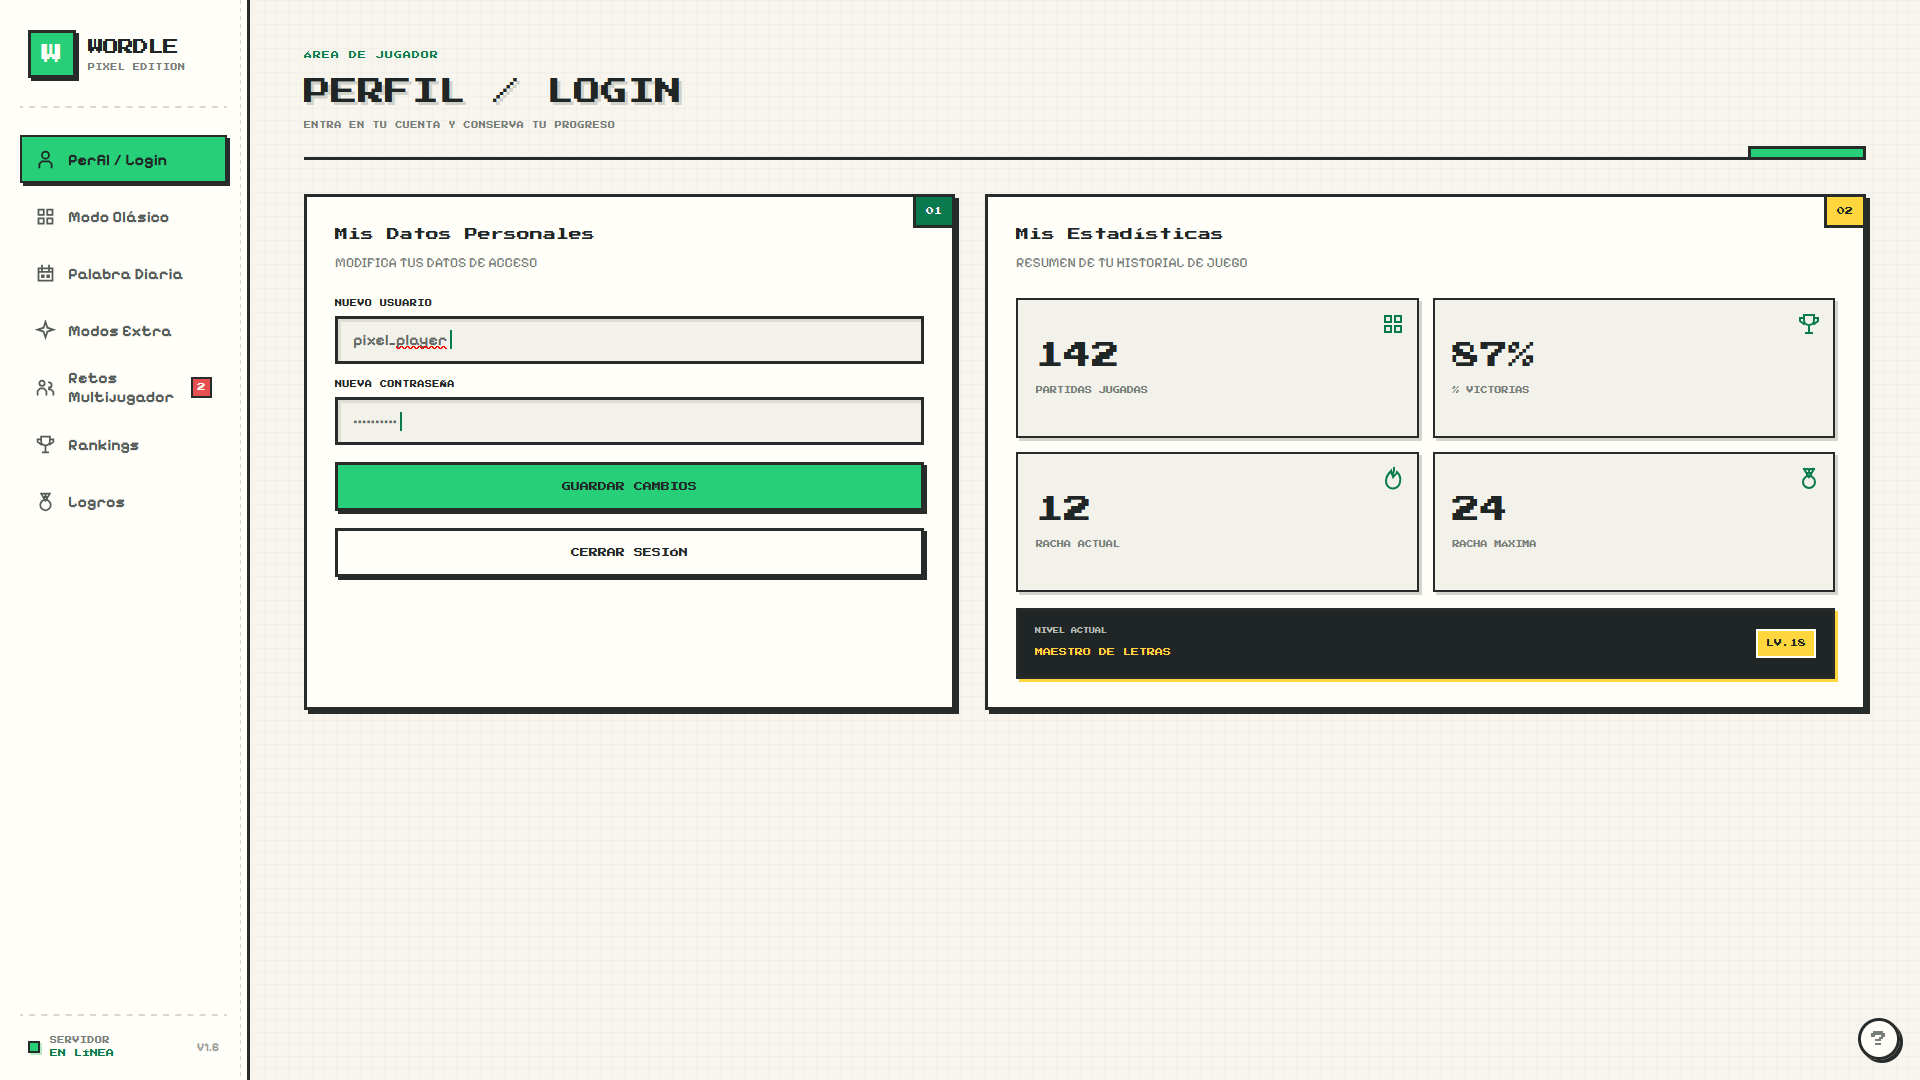
\includegraphics[width=0.85\linewidth]{Mis datos.png}}
  \caption{Estadísticas personales}
  \label{fig:estadisticas-personales-detalladas}
\end{figure}}

% ===========================================================================
% FUNCIONALIDAD 6
% ===========================================================================
\clearpage
\funcionalidad{6}

\newcommand{\cduGraficoFuncSeis}{%
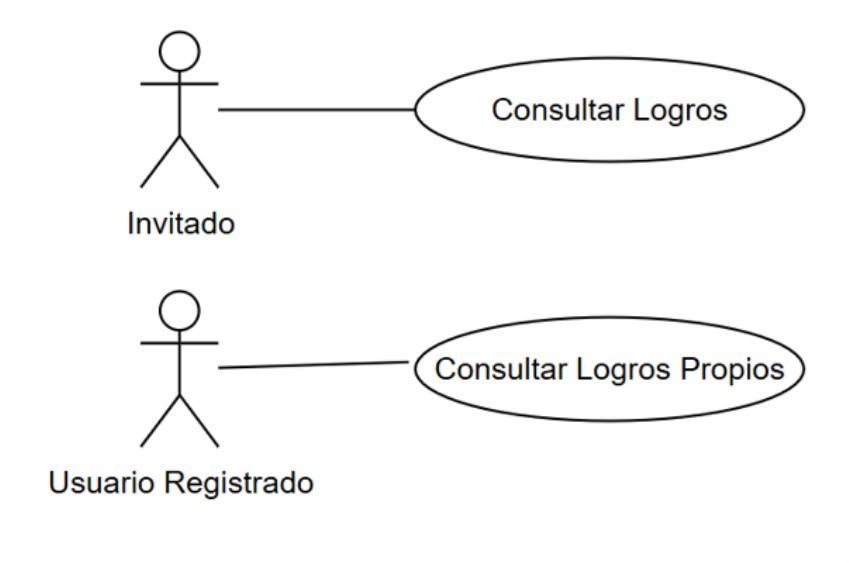
\includegraphics[
    width=0.9\linewidth,
    height=5.2cm,
    keepaspectratio
]{Funcionalidad6.jpeg}
}




\casoDeUso{\cduGraficoFuncSeis}
  {Consultar logros}
  {Permite consultar los logros especificando: Nombre del logro y los usuarios que lo han conseguido.}
  {Invitado, usuario registrado}
  {Ninguna.}
  {Ninguno.}
  {\begin{enumerate}
    \item Selecciona la opción "Consultar logros" (Ilustración 25).
    \item Se muestra el listado de logros del juego.
    \item Si se pulsa en un logro se visualiza un listado reducido de los usuarios que lo han conseguido.
  \end{enumerate}}
  {Ninguna.}
{\begin{figure}[H]
  \centering
  \fbox{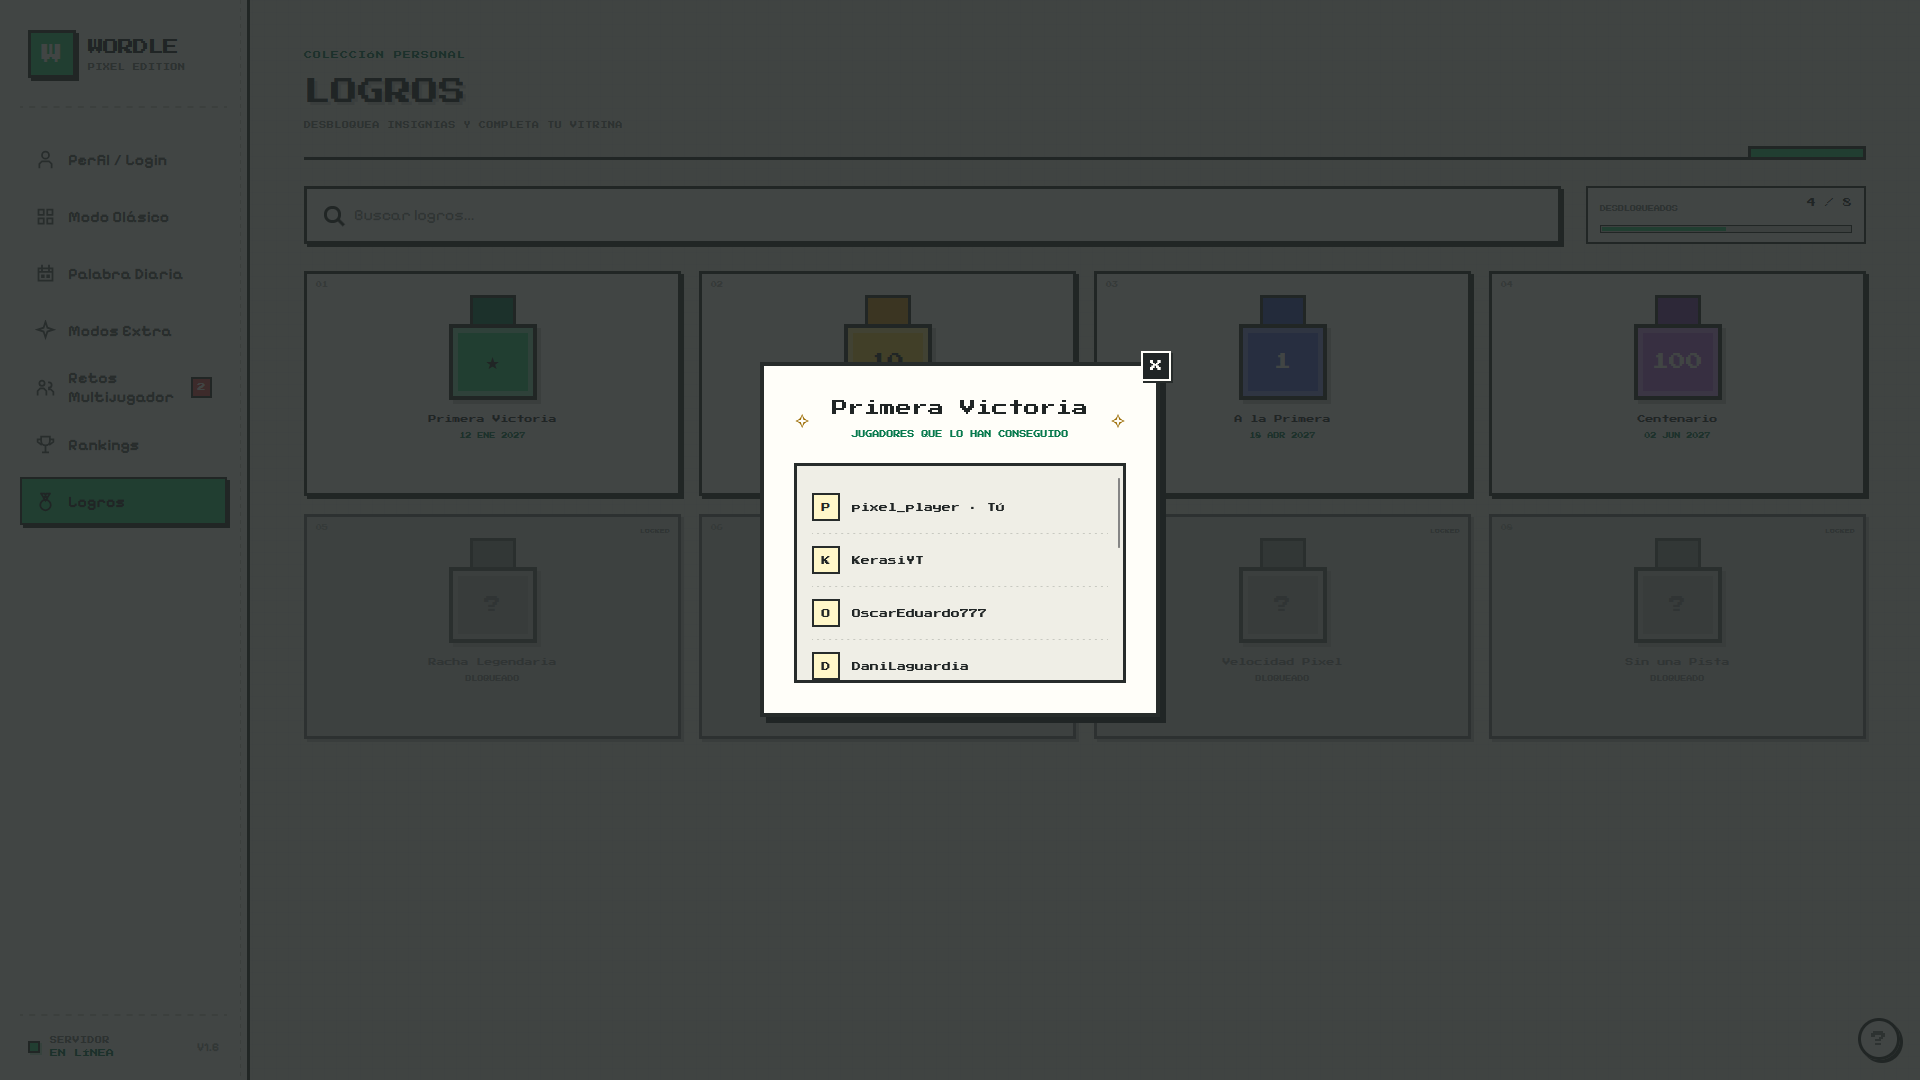
\includegraphics[width=0.85\linewidth]{Lista usuarios logros.png}}
  \caption{Logros}
  \label{fig:logros}
\end{figure}}

\clearpage

\casoDeUso{\cduGraficoFuncSeis}
  {Consultar logros propios}
  {Permite consultar los logros especificando: nombre del logro, logros obtenidos y fecha de obtención, y logros pendientes.}
  {Usuario registrado}
  {Estar identificado en el sistema.}
  {Ninguno.}
  {\begin{enumerate}
    \item Selecciona la opción "Mis logros".
    \item Se muestra el listado de logros obtenidos, fecha de obtención y logros pendientes (Ilustración 26).
    \item Si se pulsa en un logro se visualiza un listado reducido de los usuarios que lo han conseguido.
  \end{enumerate}}
  {Ninguna.}
{\begin{figure}[H]
  \centering
  \fbox{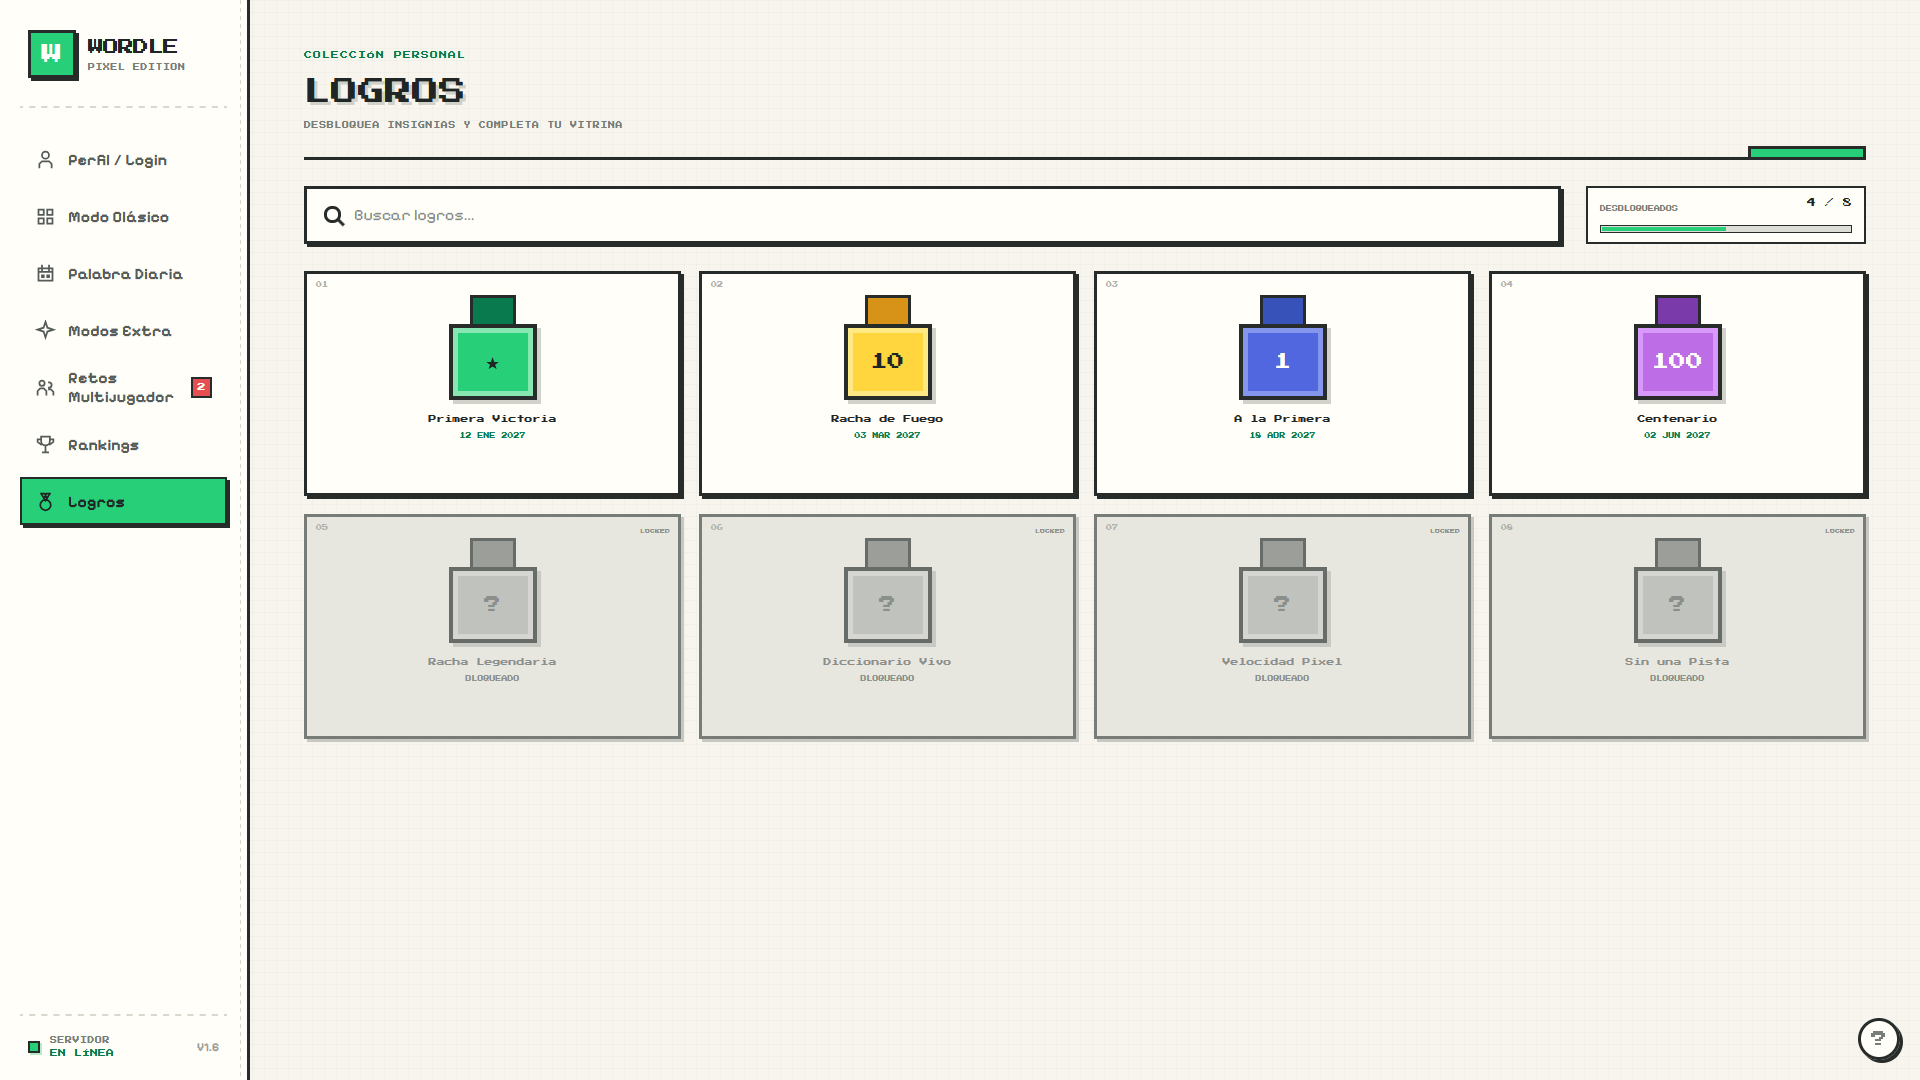
\includegraphics[width=0.85\linewidth]{Logros personales.png}}
  \caption{Logros personales}
  \label{fig:logros-personales}
\end{figure}
\begin{figure}[H]
  \centering
  \fbox{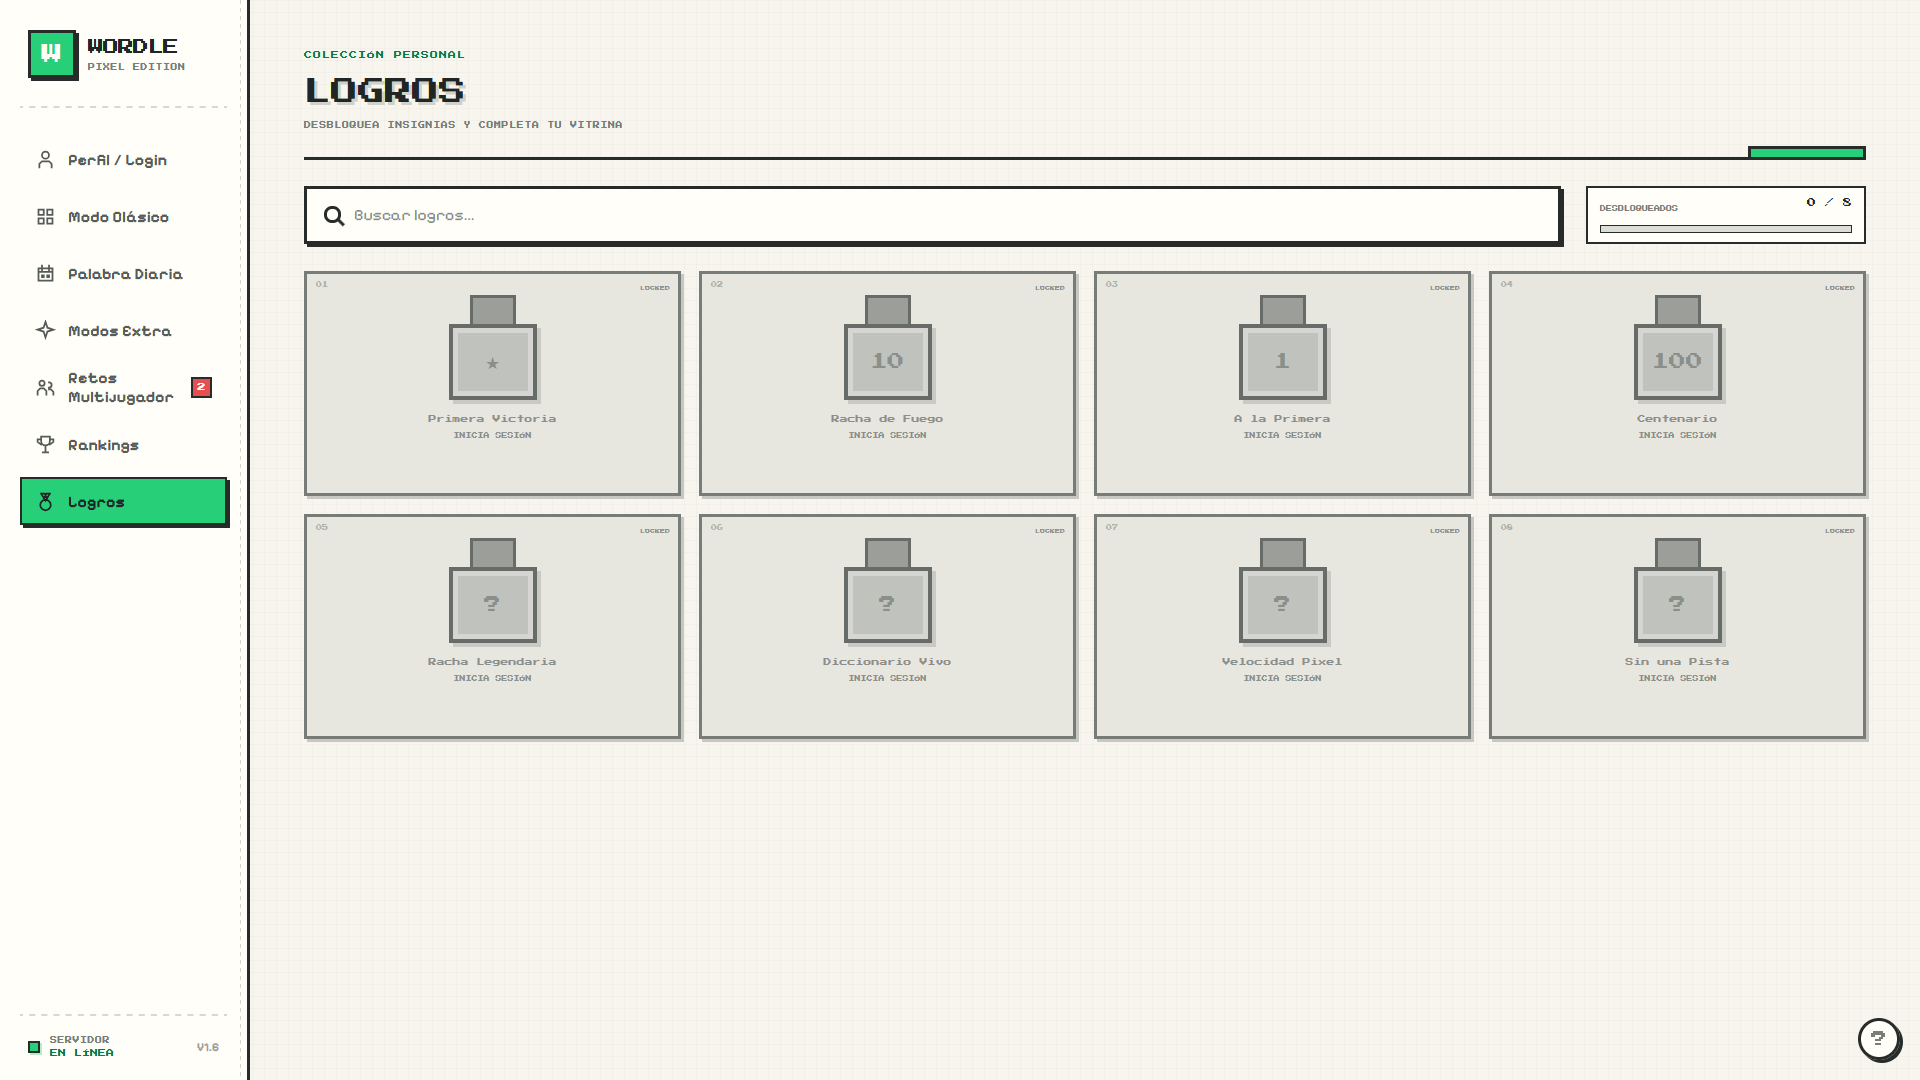
\includegraphics[width=0.85\linewidth]{Logros invitado.png}}
  \caption{Logros no disponibles para invitado}
  \label{fig:logros-invitado}
\end{figure}}

% ===========================================================================
% FUNCIONALIDAD 7
% ===========================================================================
\clearpage
\funcionalidad{7}

\newcommand{\cduGraficoFuncSiete}{%
  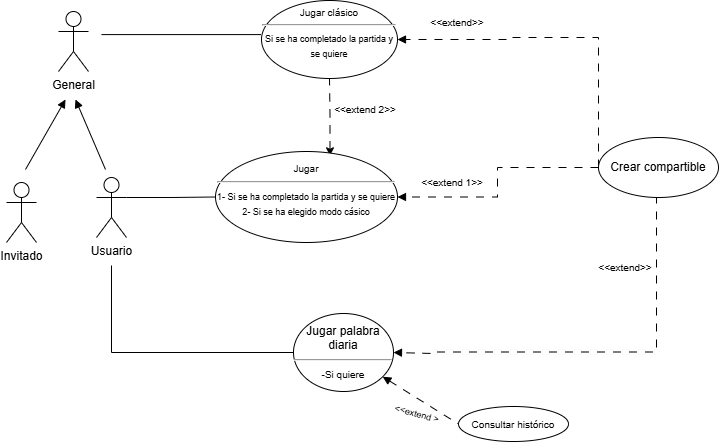
\includegraphics[
    width=0.9\linewidth,
    height=5.2cm,
    keepaspectratio
  ]{Funcionalidad7.drawio.png}%
}



\casoDeUso{\cduGraficoFuncSiete}
  {Crear compartible}
  {Al finalizar una partida el jugador tiene la opción de crear un resumen de su partida, y este se añade a su portapapeles.}
  {\textbf{General}, a través del Caso de Uso: \textit{Jugar clásico} y \textbf{Usuario}, a través de los Casos de Uso: \textit{Jugar 2, Jugar 3 o Jugar 4}.}
  {\begin{itemize}
    \item El actor ha terminado la partida, esto es, o bien ha adivinado la palabra, o ha gastado todos sus intentos (Ilustración 28).
    \item Los datos siguen disponibles, no ha cerrado o cambiado a otra partida.
  \end{itemize}}
  {\begin{itemize}
      \item El resumen debe copiarse de manera inmediata tras pulsar el botón.
  \end{itemize}}
  {\begin{enumerate}
\item El sistema muestra el resultado de la partida (Ilustración 28, 29 y 30).
\item El actor pulsa el botón de Crear Compartible. (En los cuatro modos de juegos el botón es igual, y si no ha terminado la partida no copia nada).
\item El sistema obtiene los datos de la partida recién jugada.
\item El sistema genera un resumen con los datos de la partida.
\item El resumen se copia al portapapeles (Ilustración 28).
\item El sistema muestra el mensaje: Resumen copiado al portapapeles.
  \end{enumerate}}
  {El usuario tiene en su portapapeles el compartible con la información que desea de la partida.}
{\begin{figure}[H]
  \centering
  \fbox{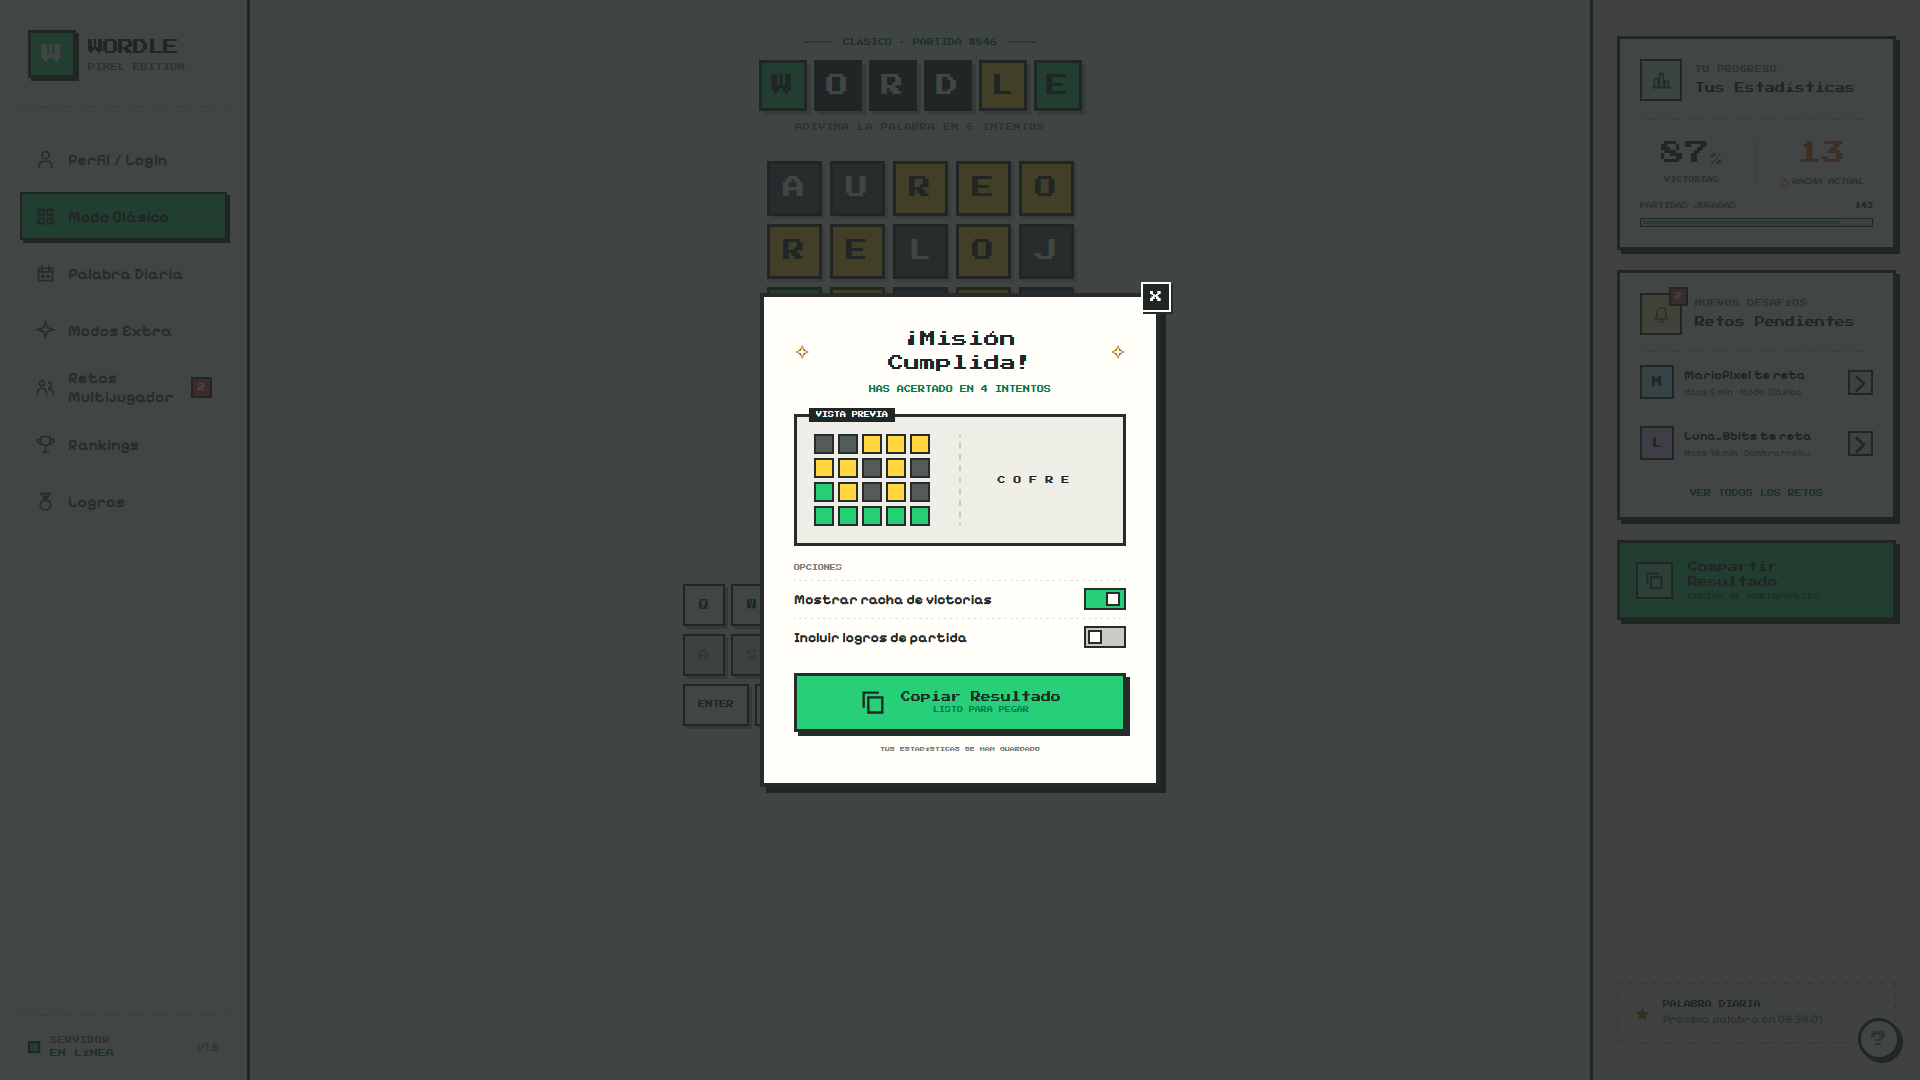
\includegraphics[width=0.6\linewidth]{Clasico completado.png}}
  \caption{Compartir partida victoriosa}
  \label{fig:compartir-victoria}
\end{figure}
\begin{figure}[H]
  \centering
  \fbox{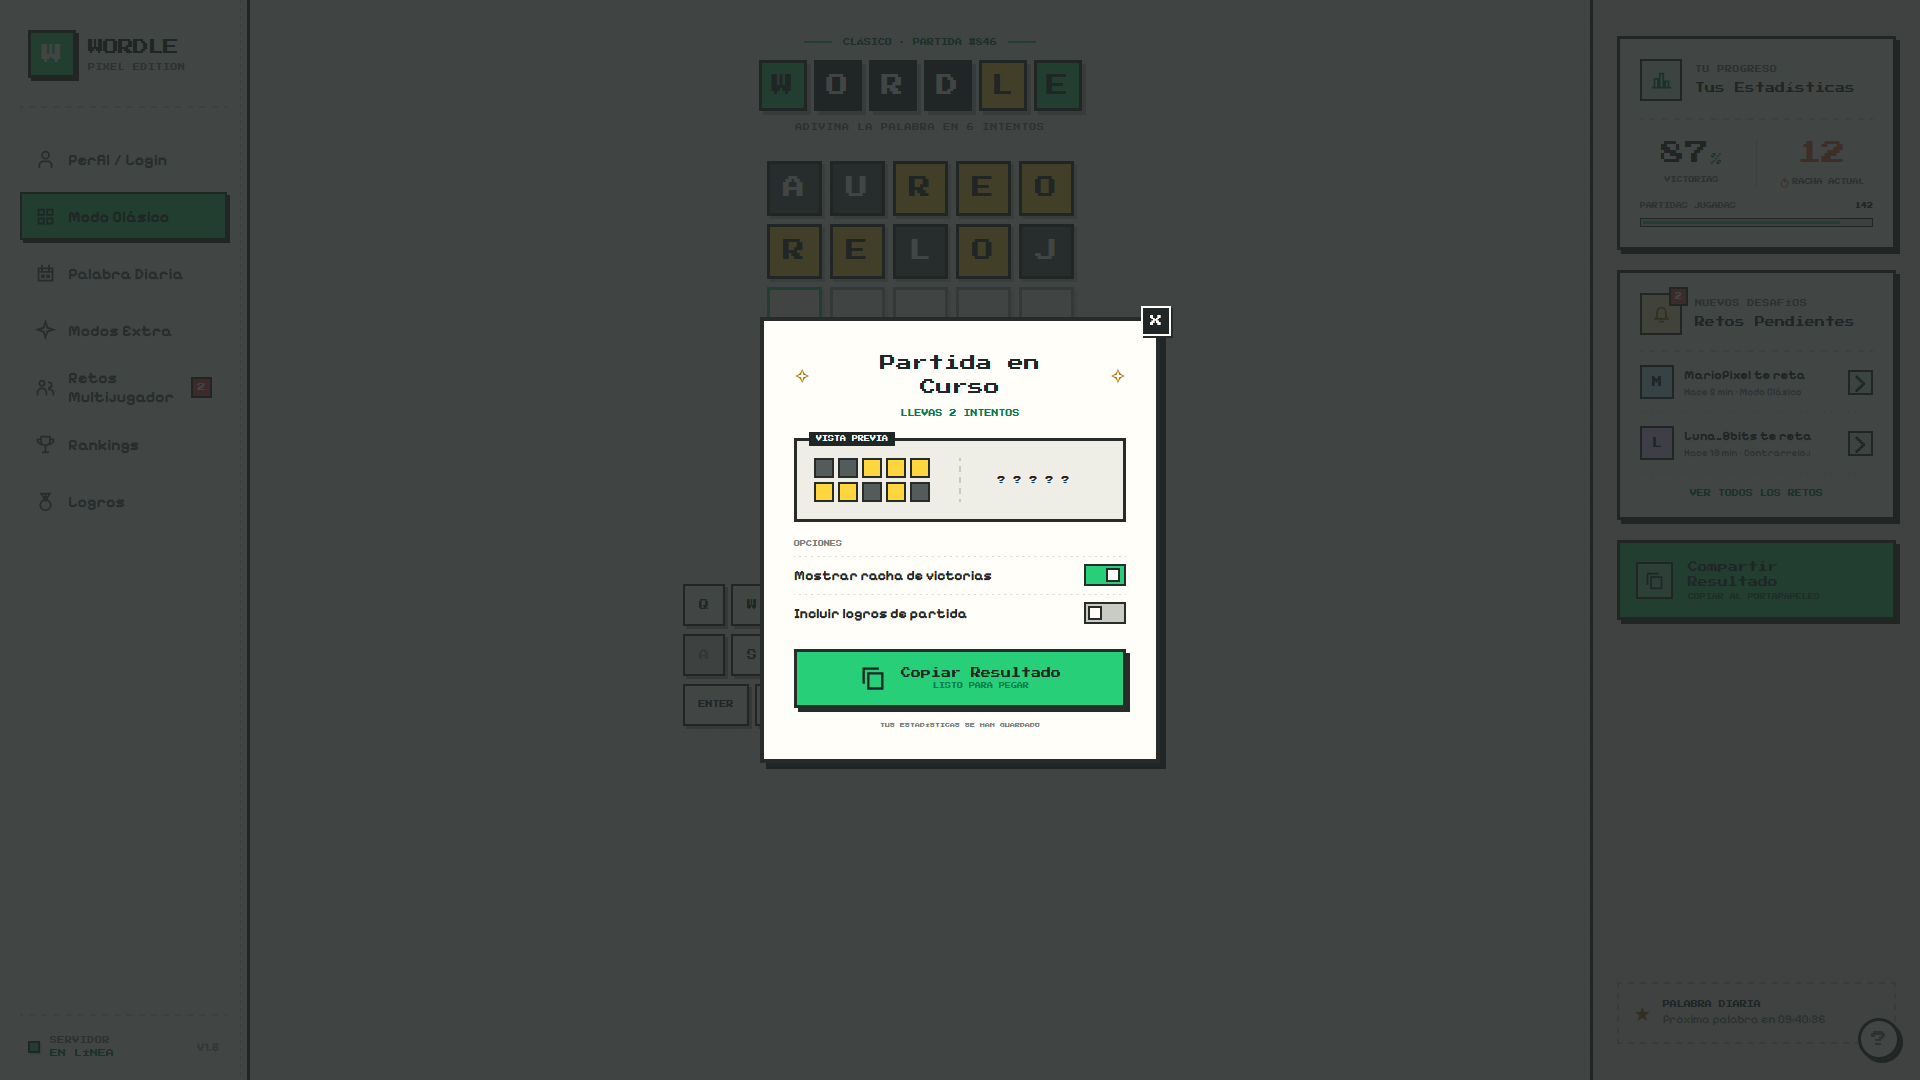
\includegraphics[width=0.6\linewidth]{Clasico en curso compartir.png}}
  \caption{Compartir no disponible para partida en curso}
  \label{fig:compartir-en-curso}
\end{figure}
\begin{figure}[H]
  \centering
  \fbox{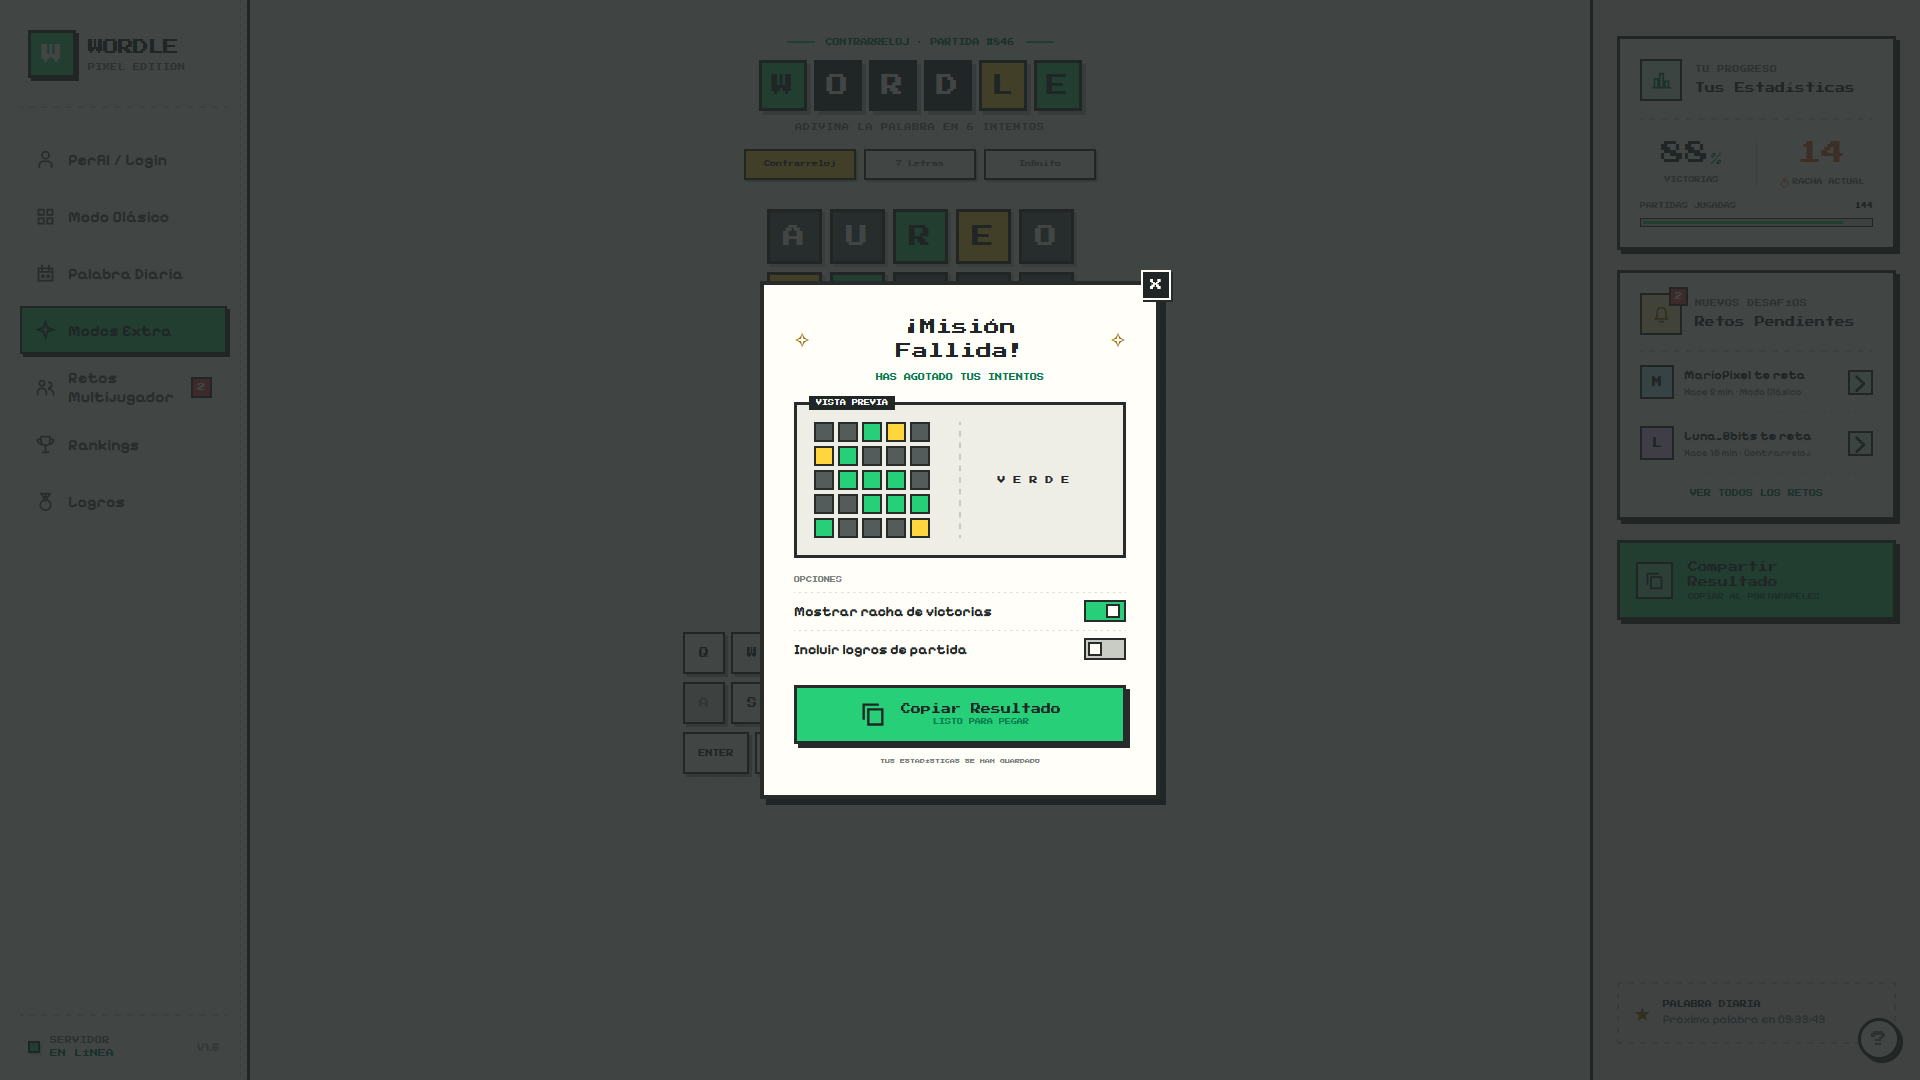
\includegraphics[width=0.6\linewidth]{Contrareloj game over.png}}
  \caption{Compartir partida fallida}
  \label{fig:compartir-fallida}
\end{figure}}

% ===========================================================================
% MODELO DE DOMINIO
% ===========================================================================
\clearpage
\fancyhead[C]{}
\section{Modelo de dominio}
\label{sec:introduccion}


\subsection{Diagrama del modelo de dominio}
\begin{figure}[h]
    \centering
  \fbox{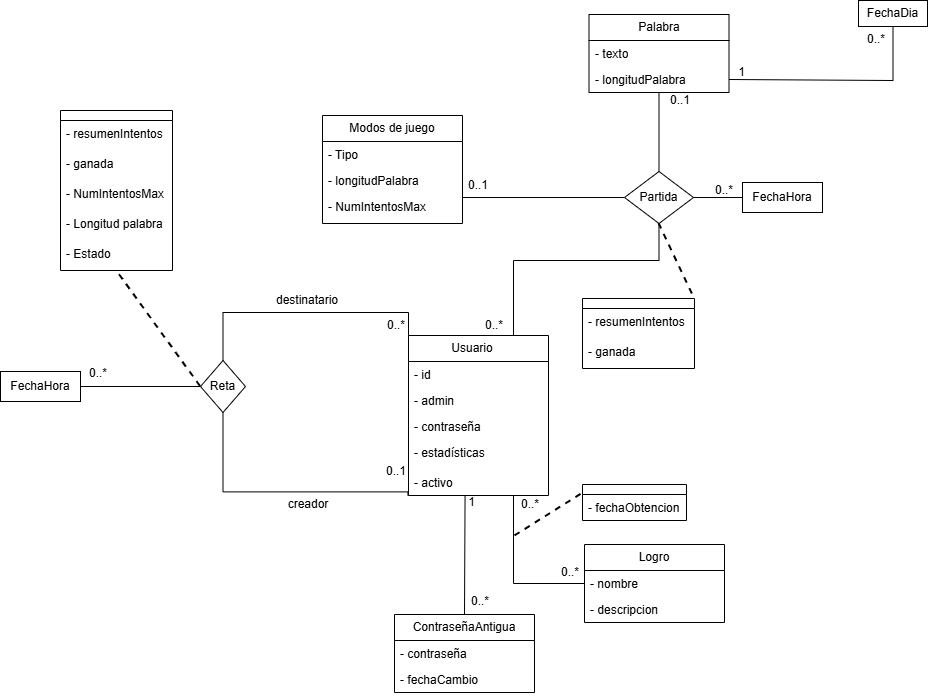
\includegraphics[width=1\linewidth]{imagenes/ModeloDominio.png}}
    \caption{Diagrama del modelo de dominio}
    \label{fig:diagrama}
\end{figure}

\clearpage

\subsection{Descripción del modelo de dominio}

El modelo de dominio representa los elementos principales del sistema Wordle, sus características y las relaciones que existen entre ellos. A continuación, se describen las entidades que aparecen en el diagrama y las relaciones que permiten explicar cómo funciona el sistema.


\subsubsection{Entidades principales}

\noindent\textbf{Palabra}

Representa una palabra que puede utilizarse como solución en una partida de Wordle. Cada palabra tiene los siguientes atributos:

\begin{itemize}
    \item \texttt{texto}: almacena el contenido de la palabra.
    \item \texttt{longitudPalabra}: indica el número de caracteres que tiene.
\end{itemize}

\par\vspace{0.5cm}
\noindent\textbf{Modos de juego}

Representa los diferentes tipos de juego a los que el usuario puede optar a jugar, Cada Modo de juego tiene los siguientes atributos:

\begin{itemize}
    \item \texttt{tipo}: indica el nombre del modo de juego.
    \item \texttt{longitudPalabra}: indica el número de letras que contiene la palabra.
    \item \texttt{numIntentosMax}: establece el número máximo de intentos permitidos para esa partida.
\end{itemize}

\par\vspace{0.5cm}
\noindent\textbf{FechaHora}

Representa una fecha concreta del calendario. Se utiliza para identificar el dia y la hora relacionada con cada reto.

\par\vspace{0.5cm}
\noindent\textbf{Usuario}

Representa a una persona que utiliza el sistema. Almacena sus datos de identificación y configuración:

\begin{itemize}
    \item \texttt{id}: identificador único del usuario.
    \item \texttt{admin}: indica si el usuario tiene permisos de administrador.
    \item \texttt{contraseña}: contraseña asociada a su cuenta.
    \item \texttt{estadísticas}: contiene las puntuaciones de cada jugador.
    \item \texttt{activo}: indica si la cuenta del usuario se encuentra activa.
\end{itemize}

\par\vspace{0.5cm}
\noindent\textbf{FechaHora}

Representa una fecha concreta del calendario. Se utiliza para identificar el dia y la hora relacionada con cada reto.

\par\vspace{0.5cm}
\noindent\textbf{FechaDia}

Representa una fecha concreta del calendario. Se utiliza para identificar los días en los que se ofrece la palabra diaria y las partidas correspondientes.

\par\vspace{0.5cm}
\noindent\textbf{ContraseñaAntigua}

Almacena las contraseñas anteriores de un usuario, permitiendo conservar un historial de los cambios de contraseña realizados. Sus atributos son:

\begin{itemize}
    \item \texttt{contraseña}: contraseña anterior del usuario.
    \item \texttt{fechaCambio}: fecha en la que se realizó el cambio de contraseña.
\end{itemize}

\par\vspace{0.5cm}
\noindent\textbf{Logro}

Representa un logro que puede conseguir un usuario al cumplir determinadas condiciones dentro del juego. Contiene los siguientes atributos:

\begin{itemize}
    \item \texttt{nombre}: nombre identificativo del logro.
    \item \texttt{descripcion}: explicación de las condiciones o características del logro.
\end{itemize}


\subsubsection{Relaciones}

\noindent\textbf{Partida}
Relaciona las \texttt{palabras} que se juegan en un \texttt{modo} específico a una \texttt{hora} por un \texttt{usuario}. Una palabra a un hora por un usuario solo puede ser jugado por un único modo de juego. Un modo de juego, con una palabra a una hora puede ser jugada por varios usuarios. Una palabra en un modo de juego y un usuario puede ser en varias Horas. Finalmente en un modo de juego a una hora y por un usuario, solo puede ser una única palabra. Además se guarda el resumen de intentos y si se ha ganado o perdido la partida.

\par\vspace{0.5cm}
\noindent\textbf{Palabra -- FechaDia}

Es una relación entre \texttt{Palabra} y \texttt{FechaDia}. Permite representar la palabra diaria asociada a una fecha. Una palabra puede utilizarse en distintas fechas, pero en una fecha solo se juega una palabra.

\par\vspace{0.5cm}
\noindent\textbf{Reta}

Relaciona el \texttt{creador} y el \texttt{destinatario} del reto así como la \texttt{fecha}. Representa la creación de un reto por un usuario. Un usuario puede crear crear un reto o ninguno en una hora. Un usuario puede recibir varios retos de otros usuarios a una hora. Por último un creador puede retar a un mismo destinatario en diferentes horas. Por otro lado en esta relación se almacena el resumen de intentos, si se ha ganado la partida, el número de intentos y la longitud de la palabra implicada en el reto y el estado del reto (pendiente, aceptado...).

\par\vspace{0.5cm}
\noindent\textbf{Usuario -- ContraseñaAntigua}

Relaciona cada usuario con las contraseñas que ha utilizado anteriormente. Un usuario puede tener cero o muchas contraseñas antiguas, mientras que cada contraseña antigua pertenece a un único usuario. Esta relación permite mantener un registro de las contraseñas anteriores y de sus fechas de cambio.

\par\vspace{0.5cm}
\noindent\textbf{Usuario -- Logro}

Relaciona los usuarios con los logros que consiguen durante el juego. Un usuario puede tener cero o muchos logros, de igual forma,  cada logro está asociado a cero o varios usuarios, dependiendo de cuantos consigan ese reto en concreto.

Esta relación tiene asociada \texttt{fechaObtencion}, que almacena la fecha en la que el usuario consiguió el logro. Se trata de un dato propio de la relación entre el usuario y el logro, ya que indica cuándo lo obtuvo ese usuario.



% =========================================================================
% 4. PLAN DE PRUEBAS
% =========================================================================

\clearpage
\section{Plan de pruebas}

En este apartado se recoge el plan de pruebas diseñado para comprobar
el correcto funcionamiento de las distintas funcionalidades del sistema
WORDLE. Para cada funcionalidad se detallan los casos de prueba realizados,
la descripción de cada prueba, el resultado esperado y el resultado
obtenido.

% -------------------------------------------------------------------------
% FORMATO DE LAS TABLAS DE PRUEBAS
% -------------------------------------------------------------------------

\renewcommand{\arraystretch}{1.25}
\setlength{\LTpre}{8pt}
\setlength{\LTpost}{8pt}

\newcommand{\tablaPruebas}{%
\small
\begin{longtable}{|
>{\centering\arraybackslash}p{1.1cm}|
>{\justifying\noindent\arraybackslash}p{3.5cm}|
>{\justifying\noindent\arraybackslash}p{3.5cm}|
>{\justifying\noindent\arraybackslash}p{3.0cm}|
>{\justifying\noindent\arraybackslash}p{2.0cm}|}
\hline
\textbf{ID} & \textbf{Descripción} &
\textbf{Resultado esperado} & \textbf{Resultado obtenido} &
\textbf{Observaciones} \\
\hline
\endfirsthead
\hline
\textbf{ID} & \textbf{Descripción} &
\textbf{Resultado esperado} & \textbf{Resultado obtenido} &
\textbf{Observaciones} \\
\hline
\endhead
}

% =========================================================================
% FUNCIONALIDAD 1: IDENTIFICACIÓN Y PERFIL
% =========================================================================

\subsection{Funcionalidad 1 («Identificación y perfil»)}
\label{sec:funcionalidad1}

\textbf{Responsable:} Aitor de Miguel Marqués

\tablaPruebas

F1-01 &
Se introduce el usuario correctamente, pero se mete la contraseña mal. &
Se muestra un mensaje de error. &
Se muestra un mensaje de error. &
Correcto. \\
\hline

F1-02 &
Se introduce la contraseña bien, pero el usuario mal. &
Se muestra un mensaje de error. &
Se muestra un mensaje de error. &
Correcto. \\
\hline

F1-03 &
Se mete el usuario correcto junto a la contraseña adecuada. &
Se da acceso a las funcionalidades del usuario identificado. &
Se da acceso a las funcionalidades del usuario identificado. &
Correcto. \\
\hline

F1-04 &
El administrador tiene la opción funcional de dar de baja a un usuario. &
El usuario no puede volver a identificarse, y le sale un mensaje explicando la situación. &
El usuario no puede volver a identificarse, y le sale un mensaje explicando la situación. &
Correcto. \\
\hline

F1-05 &
El administrador trata de eliminar a un usuario con poderes de administrador. &
Se muestra un mensaje diciendo que no se puede hacer. &
Se muestra un mensaje diciendo que no se puede hacer. &
Correcto. \\
\hline

F1-06 &
El administrador trata de jugar a cualquier modo de juego. &
Accede al juego como cualquier usuario normal. &
Accede al juego como cualquier usuario normal. &
Correcto \\
\hline

F1-07 &
Al registrarse ya existe el usuario. &
Se muestra mensaje de error indicando el motivo. &
Se muestra mensaje de error indicando el motivo. &
Correcto. \\
\hline

F1-08 &
Los datos del registro son correctos. &
Se accede a la interfaz del usuario identificado. &
Se accede a la interfaz del usuario identificado. &
Correcto. \\
\hline

F1-09 &
Al cambiar la contraseña la contraseña actual está mal. &
Se muestra un mensaje de error. &
Se muestra un mensaje de error. &
Correcto. \\
\hline

F1-10 &
Al cambiar la contraseña la confirmación difiere de la nueva contraseña. &
Se muestra un mensaje de error. &
Se muestra un mensaje de error. &
Correcto. \\
\hline

F1-11 &
Al cambiar la contraseña, la nueva no cumple los requisitos previos (no repetir antiguas). &
Se muestra un mensaje de error. &
Se muestra un mensaje de error. &
Correcto. \\
\hline

F1-12 &
Todos los datos del cambio de contraseña son correctos. &
Se muestra un mensaje de datos actualizados, se actualiza la contraseña, y se añade la anterior a contraseñas antiguas. &
Se muestra un mensaje de datos actualizados, se actualiza la contraseña, y se añade la anterior a contraseñas antiguas. &
Correcto. \\
\hline

F1-13 &
Se trata de cambiar la contraseña a una que es igual a la acutal. &
Se muestra un mensaje de error explicativo. &
Se muestra un mensaje de error explicativo. &
Correcto. \\
\hline

F1-14 &
Se va a la pestaña de ver el perfil de un usuario identificado. &
Se muestran sus datos correctos. &
Se muestran sus datos correctos. &
Correcto. \\
\hline

\end{longtable}

\tablaPruebas

F2-01 &
Usuario invitado accede al "Modo clásico" y envía la palabra "AUDIO" (Palabra válida: 5 letras). &
El tablero procesa el intento y asigna los colores correctamente: Letra correcta y en posición, verde; letra correcta en posición incorrecta, amarilla; letra incorrecta, gris. &
El tablero procesa el intento y los colores se asignan correctamente tras validar el intento. &
Correcto. \\
\hline

F2-02 &
Usuario invitado o identificado en "Modo clásico" intenta enviar una palabra de 4 letras "CASA". &
El sistema rechaza el envío sin consumir el intento y solicita completar la fila. &
El sistema rechaza el envío y no resta intento. &
Se comprueba el límite inferior. \\
\hline

F2-03 &
Usuario invitado o identificado en "Modo clásico" intenta introducir una 6ª letra tras escribir "CAMPO". &
El sistema bloquea la entrada por teclado, no permitiendo sobrepasar las 5 casillas. &
El sistema bloquea teclado tras la 5ª letra. &
Se comprueba el límite superior. \\
\hline

F2-04 &
Usuario invitado o identificado en "Modo clásico" intenta introducir números "12345" o caracteres "@@@@" (caracteres inválidos). &
El sistema ignora los caracteres alfanuméricos/símbolos y las casillas quedan vacías. &
El sistema ignora entradas no alfabéticas. &
Verificación de tipo de dato. \\
\hline

F2-05 &
Usuario invitado o identificado en "Modo clásico" intenta enviar "AAAAA" (palabra no recogida en el diccionario). &
El sistema impide el envío, muestra un aviso ("Palabra no válida") y no resta el intento. &
Impide el envío y muestra aviso por pantalla. &
Verificación de diccionario. \\
\hline

F2-06 &
Usuario invitado adivina la palabra en el "Modo clásico" en el intento 3. &
Mensaje de victoria. El sistema no almacena ningún dato. &
Tan solo se muestra mensaje de victoria. &
Correcto. \\
\hline

F2-07 &
Usuario identificado adivina la palabra en el "Modo clásico" en el intento 3. &
Mensaje de victoria. Se guarda en el historial: fecha, 3 intentos y estado visual de la cuadrícula. &
Mensaje de victoria y almacenamiento completo en historial. &
Correcto. \\
\hline

F2-08 &
Usuario invitado en "Modo clásico" falla la palabra consumiendo su intento 6 (máx. de intentos). &
Mensaje de derrota inmediatamente tras la fila 6. El sistema no almacena ningún dato. &
Tan solo se muestra mensaje de derrota. &
Correcto. \\
\hline

F2-09 &
Usuario identificado en "Modo clásico" falla la palabra consumiendo su intento 6 (máx. de intentos). &
Mensaje de derrota tras la fila 6. Se guarda en el historial: fecha, 6 intentos y estado visual de la cuadrícula. &
Mensaje de derrota y almacenamiento en historial. &
Correcto. \\
\hline

F2-10 &
Usuario invitado intenta seleccionar el modo "Contrarreloj" (sin permisos para jugar modos extra). &
Pantalla de "ACCESO DENEGADO" indicando necesidad de login. &
Pantalla de "ACCESO DENEGADO". &
Correcto. \\
\hline

F2-11 &
Usuario identificado selecciona el modo "Contrarreloj" (Jugar 2). &
El sistema permite el acceso al tablero y el temporizador inicia su cuenta regresiva. &
Acceso permitido y temporizador iniciado. &
Acceso a modo extra validado. \\
\hline

F2-12 &
Usuario identificado envía la palabra correcta en "Contrarreloj" con el temporizador en "00:15". &
Mensaje de victoria. Se guarda en el historial: fecha, intentos, estado de cuadrícula y el tiempo empleado. &
Mensaje de victoria y almacenamiento del tiempo en historial. &
Correcto. \\
\hline

F2-13 &
Usuario identificado en "Contrarreloj" intenta enviar "BBBBB" (palabra no recogida en el diccionario). &
El sistema impide el envío, muestra un aviso ("Palabra no válida") y no resta el intento. &
Impide el envío y muestra aviso por pantalla. &
Verificación de diccionario. \\
\hline

F2-14 &
Usuario identificado en "Contrarreloj" intenta enviar una palabra con el temporizador en "00:00" exacto. &
La partida finaliza inmediatamente en derrota bloqueando el envío. Se registra en el historial. &
Partida finaliza en derrota automática. &
Correcto. \\
\hline

F2-15 &
Usuario identificado en "Contrarreloj" agota los 6 intentos antes de que el temporizador llegue a cero. &
La partida finaliza en derrota. El cronómetro se detiene y se registra la partida en el historial. &
Partida finaliza en derrota por intentos. &
Correcto. \\
\hline

F2-16 &
Usuario invitado intenta acceder al modo "7 Letras" (sin permisos para jugar modos extra). &
Pantalla de "ACCESO DENEGADO". &
Pantalla de "ACCESO DENEGADO". &
Correcto. \\
\hline

F2-17 &
Usuario identificado selecciona el modo "7 Letras" (Jugar 3). &
El sistema permite el acceso y genera un tablero adaptado con filas de 7 casillas. &
Acceso permitido a tablero de 7 casillas. &
Acceso a modo extra validado. \\
\hline

F2-18 &
Usuario identificado en "7 Letras" intenta enviar "CCCCCCC" (palabra no recogida en el diccionario). &
El sistema impide el envío, muestra un aviso ("Palabra no válida") y no resta el intento. &
Impide el envío y muestra aviso por pantalla. &
Verificación de diccionario. \\
\hline

F2-19 &
Usuario identificado en modo "7 Letras" intenta enviar una palabra de 6 letras "CAMINO". &
El sistema impide el envío y exige completar las 7 casillas de la fila. &
Impide el envío tener 7 letras. &
Se comprueba hasta el límite inferior en modo 3. \\
\hline

F2-20 &
Usuario identificado en modo "7 Letras" intenta introducir una 8ª letra. &
El sistema bloquea la entrada por teclado, no permitiendo sobrepasar las 7 casillas. &
El sistema bloquea teclado tras la 7ª letra. &
Se comprueba el límite superior en modo 3. \\
\hline

F2-21 &
Usuario identificado adivina la palabra "TECLADO" correctamente en el modo "7 Letras". &
Mensaje de victoria y almacenamiento de intentos y cuadrícula en el historial. &
Victoria registrada en el historial. &
Correcto. \\
\hline

F2-22 &
Usuario identificado en el modo "7 Letras" falla la palabra consumiendo su intento 6 (máx. de intentos). &
Mensaje de derrota tras la fila 6. Se guarda en el historial: fecha, 6 intentos y estado visual de la cuadrícula. &
Mensaje de derrota y almacenamiento en historial. &
Correcto. \\
\hline

F2-23 &
Usuario invitado intenta acceder al modo "Infinito" (sin permisos para jugar modos extra). &
Pantalla de "ACCESO DENEGADO". &
Pantalla de "ACCESO DENEGADO". &
Correcto. \\
\hline

F2-24 &
Usuario identificado selecciona el modo "Infinito" (Jugar 4). &
El sistema permite el acceso al tablero en modalidad continua, inicializando la racha a 0. &
Acceso permitido en modalidad infinita. &
Acceso a modo extra validado. \\
\hline

F2-25 &
Usuario identificado en "Infinito" intenta enviar "DDDDD" (palabra no recogida en el diccionario). &
El sistema impide el envío, muestra un aviso ("Palabra no válida") y no resta el intento. &
Impide el envío y muestra aviso por pantalla. &
Verificación de diccionario. \\
\hline

F2-26 &
Usuario identificado acierta la primera palabra de 5 letras en el intento 4 en modo "Infinito". &
El tablero se limpia, la racha aumenta su valor (pasa a 1), los intentos se acumulan y aparece nueva palabra. &
Tablero se limpia, contador de racha aumenta. &
Transición de palabra validada. \\
\hline

F2-27 &
Usuario identificado en modo "Infinito" con racha=3 agota los 6 intentos en la nueva palabra. &
Mensaje de derrota. Se guarda en el historial: racha final (3) y media de intentos. &
Fin de partida y registro de racha obtenida. &
Correcto. \\
\hline

\end{longtable}


% =========================================================================
% FUNCIONALIDAD 3: PALABRA DIARIA
% =========================================================================

\section{Funcionalidad 3 («Palabra diaria»)}
\label{sec:funcionalidad3}

\textbf{Responsable:} David Martínez García

\tablaPruebas

F3-01 &
Usuario no registrado pulsa en el modo de juego de partida diaria. &
Mensaje de error, login necesario. &
Mensaje de error, login necesario. &
Correcto. \\
\hline

F3-02 &
Usuario registrado pulsa en el modo de juego de partida diaria. &
Entra a la modalidad palabra diaria. &
Entra a la modalidad palabra diaria. &
Correcto. \\
\hline

F3-03 &
Usuario Registrado entra a historico de resultados. &
Entra a resultados historicos. &
Entra a resultados historicos. &
Correcto. \\
\hline

F3-04 &
Usuario Registrado pulsa en jugar partida y esta ya está resuelta. &
Mensaje de palabra diaria resuelta. &
Mensaje de palabra diaria resuelta. &
Correcto. \\
\hline

F3-05 &
Usuario Registrado pulsa en jugar partida y esta no está resuelta. &
Entra en el modo partida diaria sin estar completado. &
Entra en el modo partida diaria sin estar completado. &
Correcto. \\
\hline

F3-06 &
Usuario Registrado introduce una palabra válida como intento durante la partida. &
Se guarda el progreso registrando la palabra introducida. &
Se guarda el progreso registrando la palabra introducida. &
Correcto. \\
\hline

F3-07 &
Usuario introduce una palabra que no existe en el diccionario interno del juego. &
Mensaje de error indicando que la palabra no es válida. &
Mensaje de error indicando que la palabra no es válida. &
Correcto. \\
\hline

F3-08 &
Usuario introduce una palabra que no es de las letras requeridas. &
Mensaje de error indicando que la palabra no es válida. &
Mensaje de error indicando que la palabra no es válida. &
Correcto. \\
\hline

F3-09 &
Usuario Registrado sale a otra pestaña a mitad de partida y vuelve a entrar al Juego Diario. &
El progreso de la partida (las palabras ya introducidas) se mantiene guardado. &
El progreso de la partida (las palabras ya introducidas) se mantiene guardado. &
Correcto. \\
\hline

F3-10 &
Usuario Registrado acierta la palabra diaria antes de agotar los intentos. &
Finaliza el juego y se guarda el registro (fecha inicio, resuelto correctamente y número de intentos). &
Finaliza el juego y se guarda el registro (fecha, resuelto correctamente y número de intentos). &
Correcto. \\
\hline

F3-11 &
Usuario Registrado agota todos los intentos sin acertar la palabra diaria. &
Finaliza el juego y se guarda el registro (fecha inicio, no resuelto correctamente y número de intentos agotados). &
Finaliza el juego y se guarda el registro (fecha, no resuelto correctamente y número de intentos agotados). &
Correcto. \\
\hline

F3-12 &
Usuario Registrado consulta el histórico inmediatamente después de finalizar la partida de hoy. &
El histórico se actualiza mostrando el resultado de la partida actual (fecha, resultado e intentos). &
El histórico se actualiza mostrando el resultado de la partida actual (fecha, resultado e intentos). &
Correcto. \\
\hline

F3-13 &
Validación de acierto: la letra es correcta y está en la posición correcta. &
La casilla correspondiente se ilumina en color verde. &
La casilla correspondiente se ilumina en color verde. &
Correcto. \\
\hline

F3-14 &
Validación de acierto parcial: la letra es correcta pero está en una posición incorrecta. &
La casilla correspondiente se ilumina en color amarillo. &
La casilla correspondiente se ilumina en color amarillo. &
Correcto. \\
\hline

F3-15 &
Validación de fallo: la letra introducida no se encuentra en la palabra a adivinar. &
La casilla correspondiente se oscurece (gris oscuro o negro). &
La casilla correspondiente se oscurece (gris oscuro o negro). &
Correcto. \\
\hline

F3-16 &
Usuario intenta introducir caracteres especiales, espacios o números. &
El sistema bloquea o ignora la entrada de caracteres que no sean letras del abecedario. &
El sistema bloquea o ignora la entrada de caracteres que no sean letras del abecedario. &
Correcto. \\
\hline

F3-17 &
El usuario mantiene la sesión abierta y la pantalla activa justo cuando ocurre el cambio de día (medianoche). &
El sistema permite al usuario jugar la partida en la que se encuentra, en el momento en que el juego termine y salga al menú, podrá jugar la partida diaria del día correspondiente. &
El sistema permite al usuario jugar la partida en la que se encuentra, en el momento en que el juego termine y salga al menú, podrá jugar la partida diaria del día correspondiente. &
Correcto \\
\hline

\end{longtable}


% =========================================================================
% FUNCIONALIDAD 4: RETOS ENTRE USUARIOS
% =========================================================================

\section{Funcionalidad 4 («Retos entre usuarios»)}
\label{sec:funcionalidad4}

\textbf{Responsable:} Lucía Sagasti Martínez

\tablaPruebas

F4-01 &
Un usuario intenta crear un reto y el destinatario no existe. &
Aparece un mensaje indicando que el destinatario introducido no existe. &
Aparece un mensaje indicando que el destinatario introducido no existe. &
Correcto \\
\hline

F4-02 &
Un usuario intenta crear un reto dirigido a sí mismo. &
Aparece un mensaje de error indicando que el destinatario no es válido. &
Aparece un mensaje de error indicando que el destinatario no es válido. &
Correcto \\
\hline

F4-03 &
Un usuario intenta crear un reto sin introducir alguno de los campos obligatorios. &
Aparece un mensaje de error indicando que debe rellenar todos los campos para poder crear el reto. &
Aparece un mensaje de error indicando que debe rellenar todos los campos para poder crear el reto. &
Correcto \\
\hline

F4-04 &
Un usuario intenta crear un reto y la fecha introducida no es válida. &
Aparece un mensaje indicando que la fecha es incorrecta. &
Aparece un mensaje indicando que la fecha es incorrecta. &
Correcto \\
\hline

F4-05 &
Un usuario intenta crear un reto y el número de intentos introducidos está fuera de los límites permitidos. &
Aparece un mensaje indicando que el número de intentos no es válido. &
Aparece un mensaje indicando que el número de intentos establecidos no es válido. &
Correcto \\
\hline

F4-06 &
Un usuario intenta crear un reto y la palabra introducida no es una palabra válida. &
Aparece un mensaje indicando que la palabra introducida no es una palabra válida. &
Aparece un mensaje indicando que la palabra introducida no es una palabra válida. &
Correcto \\
\hline

F4-07 &
Un usuario intenta crear el reto y todos los apartados son correctos, es decir, el destinatario existe y la fecha, el número de intentos y la palabra son válidas. &
Aparece un mensaje indicando que el reto se ha creado correctamente. &
Aparece un mensaje indicando que el reto se ha creado correctamente. &
Correcto \\
\hline

F4-08 &
El reto se caduca y se elimina de la lista de retos pendientes. &
Se muestra la lista de retos que quedan pendientes, en caso de que los haya. En la que no aparece el reto caducado. &
Se muestra la lista de retos que quedan pendientes, en caso de que los haya. En la que no aparece el reto caducado. &
Correcto \\
\hline

F4-09 &
Un usuario intenta acceder a un reto que acaba de caducar. &
Aparece un mensaje de error indicando que el reto ya no está disponible y se elimina el reto de la lista de retos pendientes. &
Aparece un mensaje de error indicando que el reto ya no está disponible y se elimina el reto de la lista de retos pendientes. &
Correcto \\
\hline

F4-10 &
Entrar a la pestaña de retos pendientes y que no haya ningún reto pendiente. &
Aparece un mensaje indicando que no hay ningún reto pendiente. &
Aparece un mensaje indicando que no hay ningún reto pendiente. &
Correcto \\
\hline

F4-11 &
Un usuario tras visualizar los detalles del reto decide aceptarlo. &
Se accede a la pantalla de juego. &
Se muestra la pantalla de juego. &
Correcto \\
\hline

F4-12 &
Un usuario tras visualizar los detalles del reto decide rechazarlo. &
Se muestra la lista de retos que quedan pendientes, en caso de que los haya. En la que no aparece el reto rechazado. &
Se muestra la lista de retos que quedan pendientes, en caso de que los haya. En la que no aparece el reto rechazado. &
Correcto \\
\hline

F4-13 &
Entrar a la pestaña de retos pendientes y que todos los retos sigan estando en fecha. &
Aparecen los retos sin realizar que todavía no se han caducado, en caso de que los haya. &
Aparecen los retos sin realizar que todavía no se han caducado. &
Correcto \\
\hline

F4-14 &
Un usuario quiere consultar los detalles de un reto al que le han retado. &
Aparece una pestaña con todos los detalles del reto. &
Aparece una pestaña con todos los detalles del reto. &
Correcto \\
\hline

F4-15 &
Un usuario ha creado el reto y el destinatario ha recibido la notificación. &
En la pestaña de retos pendientes aparece el nuevo reto. &
En la pestaña de retos pendientes aparece el nuevo reto. &
Correcto \\
\hline

F4-16 &
Entrar a la pestaña de retos finalizados y que solo se muestren los retos que se han completado. &
Se muestra la lista de retos finalizados, en caso de que los haya. &
Se muestra la lista de retos finalizados, en caso de que los haya. &
Correcto \\
\hline

F4-17 &
Un usuario intenta acceder a los datos de un reto ya finalizado. &
Aparece una pestaña con todos los datos del reto, es decir, si se ha ganado o perdido la partida, los intentos empleados y la fecha de finalización. &
Aparece una pestaña con todos los datos del reto, es decir, si se ha ganado o perdido la partida, los intentos empleados y la fecha de finalización. &
Correcto \\
\hline

F4-18 &
Entrar a la pestaña de retos finalizados y que no haya ningún reto finalizado. &
Aparece un mensaje indicando que no hay ningún reto finalizado. &
Aparece un mensaje indicando que no hay ningún reto finalizado. &
correcto \\
\hline

F4-19 &
El creador del reto es capaz de acceder a los resultados del reto ya finalizado. &
Aparece una pestaña con todos los datos del reto, es decir, si se ha ganado o perdido la partida, los intentos empleados y la fecha de finalización. &
Aparece una pestaña con todos los datos del reto, es decir, si se ha ganado o perdido la partida, los intentos empleados y la fecha de finalización. &
Correcto \\
\hline

\end{longtable}


% =========================================================================
% FUNCIONALIDAD 5: VISUALIZACIÓN DE RANKINGS Y ESTADÍSTICAS
% =========================================================================

\section{Funcionalidad 5 («Visualización de rankings y estadísticas»)}
\label{sec:funcionalidad5}

\textbf{Responsable:} Daniela Corrales Ibáñez

\tablaPruebas

F5-01 &
Ningun jugador en el mundo ha jugado nunca al juego y se consulta el ranking Global &
Aparece un mensaje indicando que el ranking Global no esta disponible &
Aparece un mensaje indicando que el ranking Global no esta disponible &
Correcto \\
\hline

F5-02 &
Uno o más jugadores han jugado alguna vez y el usuario consulta el ranking Global &
Muestra la lista de jugadores ordenados por puntos a nivel mundial &
Muestra la lista de jugadores ordenados por puntos a nivel mundial &
Correcto \\
\hline

F5-03 &
El usuario no elige ningun filtro al consultar el ranking Global &
Se muestra el ranking Global general sin filtros aplicados &
Se muestra el ranking Global general sin filtros aplicados &
Correcto \\
\hline

F5-04 &
Uno o más jugadores han jugado alguna vez y el usuario filtra por modo “Clasico” en el ranking Global &
Muestra la lista de jugadores ordenados por puntos a nivel mundial filtrado por el modo “Clasico” &
Muestra la lista de jugadores ordenados por puntos a nivel mundial filtrado por el modo “Clasico” &
Correcto \\
\hline

F5-05 &
Uno o más jugadores han jugado alguna vez y el usuario filtra por modo “2” en el ranking Global &
Muestra la lista de jugadores ordenados por puntos a nivel mundial filtrado por el modo “2” &
Muestra la lista de jugadores ordenados por puntos a nivel mundial filtrado por el modo “2” &
Correcto \\
\hline

F5-06 &
Uno o más jugadores han jugado alguna vez y el usuario filtra por modo “3” en el ranking Global &
Muestra la lista de jugadores ordenados por puntos a nivel mundial filtrado por el modo “3” &
Muestra la lista de jugadores ordenados por puntos a nivel mundial filtrado por el modo “3” &
Correcto \\
\hline

F5-07 &
Ningun jugador en el mundo ha jugado al modo de juego filtrado &
Aparece un mensaje indicando que el ranking Global para ese modo no esta disponible &
Aparece un mensaje indicando que el ranking Global para ese modo no esta disponible &
Correcto \\
\hline

F5-08 &
El usuario nunca ha jugado ninguna partida y consulta las estadísticas personales &
Aparece un mensaje indicando que no hay datos disponibles, junto a un mensaje incitando al juego &
Aparece un mensaje indicando que no hay datos disponibles, junto a un mensaje incitando al juego &
Correcto \\
\hline

F5-09 &
El usuario ha jugado una o más partidas y consulta las estadísticas personales &
Se muestran las estadísticas personales del jugador identificado &
Se muestran las estadísticas personales del jugador identificado &
Correcto \\
\hline

F5-10 &
El usuario no esta identificado (invitado) y quiere consultar las estadísticas personales &
El botón de estadísticas personales esta oculto y se muestra un mensaje indicando que debe registrarse para almacenar y visualizar sus estadísticas &
El botón de estadísticas personales esta oculto y se muestra un mensaje indicando que debe registrarse para almacenar y visualizar sus estadísticas &
Correcto \\
\hline

\end{longtable}


% =========================================================================
% FUNCIONALIDAD 6: LOGROS
% =========================================================================

\section{Funcionalidad 6 («Logros»)}
\label{sec:funcionalidad6}

\textbf{Responsable:} Gonzalo de Maguregui Sánchez

\tablaPruebas

F6-01 &
Usuario invitado accede a la pestaña de consultar logros para ver el nombre de los logros y los usuarios que los han conseguido. &
Se muestra el listado general de logros del juego. &
Se muestra el listado general de logros del juego. &
Correcto. \\
\hline

F6-02 &
Usuario registrado selecciona un logro específico en la lista general. &
Se visualiza un listado completo de los usuarios que han conseguido dicho logro. &
Se visualiza un listado completo de los usuarios que han conseguido dicho logro. &
Correcto. \\
\hline

F6-03 &
Usuario invitado selecciona un logro específico en la lista general. &
Se visualiza un listado reducido de los usuarios que han conseguido dicho logro. &
Se visualiza un listado reducido de los usuarios que han conseguido dicho logro. &
Correcto. \\
\hline

F6-04 &
Usuario invitado intenta acceder a la pestaña de consultar logros propios. &
Se deniega el acceso y se muestra que la opción no está disponible para invitados. &
Se deniega el acceso y se muestra que la opción no está disponible para invitados. &
Correcto. \\
\hline

F6-05 &
Usuario registrado accede a la opción "Mis logros". &
Se muestra el listado de logros obtenidos, la fecha de obtención y los logros pendientes. &
Se muestra el listado de logros obtenidos, la fecha de obtención y los logros pendientes. &
Correcto. \\
\hline

F6-06 &
Usuario registrado finaliza una partida cumpliendo la condición de ganar la primera partida. &
El sistema comprueba la condición al finalizar la partida y le otorga el logro correspondiente. &
El sistema comprueba la condición al finalizar la partida y le otorga el logro correspondiente. &
Correcto. \\
\hline

F6-07 &
Usuario registrado gana un número determinado de partidas consecutivas. &
El sistema comprueba la racha al finalizar la partida y otorga el logro por partidas consecutivas. &
El sistema comprueba la racha al finalizar la partida y otorga el logro por partidas consecutivas. &
Correcto. \\
\hline

F6-08 &
Usuario registrado acierta una palabra en el primer intento de una partida. &
Se comprueba al finalizar la partida y se le otorga el logro de acertar en el primer intento. &
Se comprueba al finalizar la partida y se le otorga el logro de acertar en el primer intento. &
Correcto. \\
\hline

F6-09 &
Usuario registrado alcanza un determinado número de partidas jugadas en total. &
Se comprueba la acumulación al finalizar la partida y se le otorga el logro asociado. &
Se comprueba la acumulación al finalizar la partida y se le otorga el logro asociado. &
Correcto. \\
\hline

F6-10 &
Usuario registrado revisa sus logros propios tras haber obtenido uno nuevo. &
El logro pasa a estar obtenido y refleja la fecha exacta en la que lo consiguió. &
El logro pasa a estar obtenido y refleja la fecha exacta en la que lo consiguió. &
Correcto. \\
\hline

F6-11 &
Usuario invitado finaliza una partida cumpliendo los requisitos de un logro (ej. ganar en el primer intento). &
El sistema no otorga ningún logro ni guarda fecha de obtención al no estar el usuario identificado. &
El sistema no otorga ningún logro ni guarda fecha de obtención al no estar el usuario identificado. &
Correcto. \\
\hline

F6-12 &
Usuario utiliza la barra de búsqueda (icono de lupa) en la pantalla para buscar un logro específico por su nombre. &
El sistema filtra dinámicamente y muestra únicamente los logros que coinciden con el texto introducido. &
El sistema filtra dinámicamente y muestra únicamente los logros que coinciden con el texto introducido. &
Correcto. \\
\hline

F6-13 &
Usuario pulsa sobre un logro recién creado o muy difícil que todavía no ha sido conseguido por ningún jugador en el sistema. &
El listado de usuarios se muestra vacío o aparece un mensaje indicando que nadie lo ha conseguido aún. &
El listado de usuarios se muestra vacío o aparece un mensaje indicando que nadie lo ha conseguido aún. &
Correcto. \\
\hline

F6-14 &
Usuario registrado finaliza una partida y cumple las condiciones de dos logros simultáneamente (ej. ganar la primera partida y acertar en el primer intento). &
El sistema evalúa al finalizar la partida y otorga ambos logros al mismo tiempo, registrando la fecha en ambos. &
El sistema evalúa al finalizar la partida y otorga ambos logros al mismo tiempo, registrando la fecha en ambos. &
Correcto. \\
\hline

F6-15 &
Usuario registrado en la pestaña "Mis logros" pulsa sobre un logro que aparece en la sección de "logros pendientes". &
Se muestra el listado completo de los otros usuarios que ya han conseguido ese logro, aunque el usuario actual no lo tenga. &
Se muestra el listado completo de los otros usuarios que ya han conseguido ese logro, aunque el usuario actual no lo tenga. &
Correcto. \\
\hline

F6-16 &
Usuario registrado abre un logro que ha sido conseguido por una cantidad masiva de usuarios (ej. +1000 jugadores). &
El sistema muestra la lista completa utilizando paginación o carga progresiva (scroll infinito) sin bloquear la interfaz ni exceder tiempos de carga aceptables. &
El sistema muestra la lista completa utilizando paginación o carga progresiva sin bloquear la interfaz. &
Prueba de estrés y usabilidad ante la nueva regla de "lista completa". \\
\hline

\end{longtable}


% =========================================================================
% FUNCIONALIDAD 7: COMPARTIR RESULTADOS
% =========================================================================

\section{Funcionalidad 7 («Compartir resultados»)}
\label{sec:funcionalidad7}

\textbf{Responsable:} Ekaitz Odriozola Díez

\tablaPruebas

F7-01 &
Usuario registrado intenta generar el resultado compartible de una partida que todavía está en curso &
El sistema no permite generar el resultado hasta que la partida haya finalizado &
El sistema no permite generar el resultado hasta que la partida haya finalizado &
Correcto \\
\hline

F7-02 &
Usuario sin identificar finaliza una partida e intenta generar un compartible &
El sistema no permite generar el resultado a los usuarios no identificados &
El sistema no permite generar el resultado a los usuarios no identificados &
Correcto \\
\hline

F7-03 &
Usuario registrado genera el resultado compartible de una partida ganada &
Se genera un resultado compartible, mostrando todos los intentos realizados sin revelar la palabra objetivo &
Se genera un resultado compartible, mostrando todos los intentos realizados sin revelar su contenido &
Correcto \\
\hline

F7-04 &
Usuario registrado genera el resultado compartible de una partida perdida &
Se genera un resultado compartible, mostrando todos los intentos realizados sin revelar la palabra objetivo &
Se genera un resultado compartible, mostrando todos los intentos realizados sin revelar su contenido &
Correcto \\
\hline

F7-05 &
Comprobar que se puede compartir el resultado generado &
Al copiar el elemento del portapapeles, este no se ve modificado o alterado &
Al copiar el elemento del portapapeles, este no se ve modificado o alterado &
Correcto \\
\hline

F7-06 &
Usuario registrado genera el resultado compartible y comprueba el número de intentos utilizados &
El número de intentos indicado coincide con los intentos realizados durante la partida &
El número de intentos indicado coincide con los intentos realizados durante la partida &
Correcto \\
\hline

F7-07 &
Usuario registrado genera el resultado compartible y ve la representación gráfica de los intentos &
El elemento muestra mediante casillas de colores el resultado de cada letra por cada intento realizado &
El elemento muestra mediante casillas de colores el resultado de cada letra por cada intento realizado &
Correcto \\
\hline

F7-08 &
Usuario registrado genera el resultado compartible y compara su contenido con los intentos realizados durante la partida &
La representación gráfica coincide con los resultados obtenidos, sin omitir, añadir ni alterar casillas &
La representación gráfica coincide con los resultados obtenidos, sin omitir, añadir ni alterar casillas &
Correcto \\
\hline

F7-09 &
Usuario registrado genera resultados compartibles de partidas en diferentes modos de juego (clásico, 7 letras) &
El elemento compartible representa los intentos de la partida, sea cual sea el modo de juego utilizado &
El elemento compartible representa los intentos de la partida, sea cual sea el modo de juego utilizado &
Correcto \\
\hline

F7-11 &
Usuario registrado genera el compartible de una partida contrarreloj &
El elemento compartible representa los intentos de la partida, y el tiempo en el que se ha resuelto en caso de ganar &
El elemento compartible representa los intentos de la partida, y el tiempo en que se ha resuelto en caso de ganar &
Correcto \\
\hline

F7-12 &
Usuario registrado genera el compartible de una partida infinito &
El elemento compartible representa los intentos medios de la partida, y el número de partidas ganadas y número total de partidas &
El elemento compartible representa los intentos medios de la partida, y el número de partidas ganadas y número total de partidas &
Correcto \\
\hline

F7-13 &
Usuario registrado genera el compartible de una partida diaria &
El elemento compartible representa los intentos de la partida, y la fecha del día &
El elemento compartible representa los intentos de la partida, y la fecha del día &
Correcto \\
\hline

\end{longtable}

% ===========================================================================
% FIN DE PLAN DE PRUEBAS
% ===========================================================================

\clearpage

% ===========================================================================
% GLOSARIO
% ===========================================================================

\clearpage
\fancyhead[C]{{\sffamily\bfseries Anexo A. Glosario}}

\appendix
\section*{Anexo A. Glosario}
\phantomsection
\addcontentsline{toc}{section}{Anexo A. Glosario}
\label{sec:glosario}

% Añade aquí los términos y sus definiciones.
\begin{description}[style=nextline,leftmargin=3.5cm,labelwidth=3.2cm]

    \item[Actor]
    Tipo de usuario o sistema externo que interactúa con el sistema y que representan roles. En el proyecto Wordle, los actores incluyen al usuario identificado, al invitado, al general y al administrador.

    \item[Administrador]
    Actor con permisos específicos para gestionar usuarios. Entre sus operaciones se encuentra la desactivación de cuentas.

    \item[Compartible]
    Resumen textual de una partida que el sistema genera al finalizarla y copia al portapapeles. Permite compartir el resultado sin revelar la palabra secreta.

    \item[Credenciales]
    Datos utilizados para identificar a un usuario, concretamente su nombre de usuario y contraseña.

    \item[Estadísticas personales]
    Datos derivados de las partidas de un usuario registrado, como el número de partidas jugadas y ganadas, el porcentaje de victorias, las rachas y la media de intentos.

    \item[Flujo de eventos]
    Secuencia de pasos que describe la interacción entre los actores y el sistema para completar un caso de uso. Puede incluir flujos alternativos o situaciones condicionadas.

    \item[Historial de partidas]
    Registro de las partidas realizadas por un usuario registrado. Puede contener la fecha, el resultado de la partida y el número de intentos utilizados.

    \item[Invitado]
    Usuario que puede acceder a determinadas funcionalidades sin disponer de una cuenta identificada. Puede jugar al modo clásico y consultar ciertas clasificaciones, pero no dispone de las estadísticas personales asociadas a una cuenta.

    \item[Logro]
    Hito que el jugador puede conseguir al cumplir determinadas condiciones durante el uso del sistema, como obtener una victoria o alcanzar una racha. Los logros pueden consultarse junto con su estado de obtención.

    \item[Media de intentos]
    Promedio de intentos empleados para completar las partidas. Es uno de los criterios utilizados para consultar las clasificaciones.

    \item[Modo clásico]
    Modalidad de juego en la que se debe adivinar una palabra de cinco letras en un máximo de seis intentos.

    \item[Modos de juego alternativos]
    Modalidades distintas del modo clásico que modifican parámetros de la partida, como la longitud de la palabra, el límite de intentos o el tiempo disponible.

    \item[Palabra diaria]
    Modalidad que propone un reto común para toda la comunidad cada día, en la que el usuario dispone de una única oportunidad para adivinar la palabra diaria y el sistema registra el resultado.

    \item[Partida]
    Sesión de juego en la que el jugador intenta adivinar la palabra propuesta. Finaliza cuando acierta la palabra o agota los intentos disponibles.

    \item[Porcentaje de victorias]
    Indicador que expresa la proporción de partidas ganadas respecto al total de partidas jugadas. Se utiliza como criterio de clasificación y análisis del rendimiento.

    \item[Precondición]
    Condición que debe cumplirse antes de ejecutar un caso de uso. Por ejemplo, determinadas operaciones del perfil requieren que el usuario haya iniciado sesión.

    \item[Poscondición]
    Resultado o estado que se espera al finalizar un caso de uso, tanto si la operación se completa correctamente como si termina sin realizar cambios.

    \item[Portapapeles]
    Área temporal del sistema que permite copiar información para pegarla posteriormente en otra aplicación. En Wordle se utiliza para copiar el resumen compartible de una partida.

    \item[Ranking]
    Clasificación de los jugadores ordenada según un criterio de rendimiento, como el porcentaje de victorias, la racha máxima o la media de intentos.

    \item[Racha actual]
    Número de victorias consecutivas que mantiene un usuario en el momento de consultar sus estadísticas.

    \item[Racha máxima]
    Mayor número de victorias consecutivas alcanzado por un usuario. Se utiliza como indicador estadístico y criterio de clasificación.

    \item[Requisito no funcional]
    Restricción o condición de calidad que debe satisfacer el sistema, por ejemplo, en materia de rendimiento, seguridad, disponibilidad o tiempo de respuesta.

    \item[Reto]
    Partida propuesta o compartida entre usuarios que permite participar en un desafío y consultar posteriormente su resultado. El documento contempla la consulta de retos finalizados y sus datos asociados.

    \item[Sesión]
    Periodo durante el cual un usuario identificado accede al sistema. La sesión permite asociar las operaciones realizadas con la cuenta correspondiente.

    \item[Usuario registrado]
    Usuario que dispone de una cuenta en el sistema y puede identificarse, pudiendo guardar su historial de partidas, consultar sus estadísticas personales y acceder a otras operaciones restringidas a usuarios registrados.

\end{description}

\end{document}